\chapter{$\Dsplus$ production in Pb-Pb collisions at $\s$ = 5.02 TeV}
\label{chap:PbPb}
In this Chapter the measurements of the $\pt$-differential yield,
the nuclear modification factor and the elliptic flow of $\Dsplus$ mesons
in Pb-Pb collisions at $\sNN = 5.02$ TeV will be presented. Data were
collected during the LHC Run2 in 2015 and recorded with a 
minimum-bias interaction trigger that required coincident signals in 
both scintillator arrays of the V0 detector. Events produced by 
the interaction of the beams with residual gas in the
vacuum pipe were rejected offline using the V0 and the ZDC 
timing information. Only events with a reconstructed primary vertex 
within $\pm 10$ cm from the centre of the ITS detector along
the beam line were analysed. The centrality classes 
used in the analysis, the corresponding 
average nuclear overlap functions $\av{\TAA}$~\cite{ALICE-PUBLIC-2015-008} 
and the number of events ($N_{\rm events}$) in each class 
are summarised in Table~\ref{tab:Nevents}. The corresponding 
integrated luminosity is $L_{\rm int}=13.04\pm0.4~\mub^{-1}$.\\
\begin{table}[!h]
	\centering
	\begin{tabular}{ccc}
	\hline
	Centrality class & $\langle\TAA\rangle$ (mb$^{-1}$)& $N_{\rm events}$\\
	\hline
	\phantom{0}0--10\% & $23.4\pm0.8$ & $10.4 \times 10^6$ \\
	30--50\% & $3.76\pm0.13$ & $20.8 \times 10^6$\\
	60--80\% & $0.417 \pm 0.026$ & $20.8 \times 10^6$\\
	\hline
	\end{tabular}		
	\caption{Average nuclear overlap function and number of events  for the three centrality classes used in the analysis.}
	\label{tab:Nevents}
\end{table}

For sake of clarity, we will start with the description of $\pt$-differential yields and $\RAA$ 
analyses and move to the analysis of elliptic flow in the second part of the Chapter. 
The results of the measurements will be discussed together in Sec.~\ref{sec:PbPbResults}.

\section{$\Dsplus$ $\pt$-differential yields}
\label{sec:YieldsAndRaa}
\subsection{Signal extraction}
\label{sec:SelectionPbPb}
$\Dspm$ mesons in Pb-Pb collisions were reconstructed 
and selected with the same strategy adopted in the analysis of pp 
collisions (see Sec.~\ref{sec:DsRecoStrategy}). The differences with respect to
the analysis performed in proton-proton collisions are due to the much larger
combinatorial background that is a consequence of the very 
high particle multiplicity in heavy-ion collisions. In particular, 
in the Pb-Pb analysis, stricter selections on the tracks 
used to build the $\Dspm$ candidates and on the geometrical selections
on the displaced decay vertex topology were applied. 
The stricter selections on the decay tracks contributed also to reduce the computing resources 
needed to build and store the candidates. \\



In Tables~\ref{tab:topologicalselections_ds_010},~\ref{tab:topologicalselections_ds_3050} 
and~\ref{tab:topologicalselections_ds_6080}, the topological selections applied 
in the 0-10$\%$, 30-50\% and 60-80$\%$ centrality classes
to extract the raw yields in different $\pt$ intervals are reported. Tighter cuts 
are needed for most central events due the larger amount of background. To give an idea, there are $\sim260 \cdot 10^9$
$\Ds$ candidates after a first loose filtering selection, i.e. before the optimised topological selection, in the 0-10\% centrality class.\\



The PID selection is the same used in the analysis of pp collisions and 
is described in Sec.~\ref{Sec:PID}. It considers a track to be 
compatible with the kaon or pion hypothesis 
if both its d$E$/d$x$ and time-of-flight are within 3$\sigma$ from the expected values. 
Tracks without a TOF signal (mostly at low momentum) are 
identified using only the TPC information and requiring a 2$\sigma$ 
compatibility with the expected d$E$/d$x$. This selection was used 
for $\pt < 8 \, \Gevc$ in the 0-10\% and 30-50\% centrality classes. 
and for the most peripheral 60-80\% class at all $\pt$. For the high $\pt$ regions
in the 0-10\% and 30-50\% classes, the looser PID selection introduced in Sec.~\ref{sec:PIDsystPP}
was applied since it provided good values of statistical significance of the extracted yields.


%Ds

\begin{table}[!h]
 \begin{center}
  \begin{tabular}{|c|c|c|c|c|}
\hline
$\pt$ (GeV/c)/variable &  [4,6] & [6,8] & [8,12] & [12,16] \\
\hline
\hline
Decay length ($\mum$)        & $>$500 & $>$500 & $>$400 & $>$400\\
\hline
Decay length XY ($\mum$)     & $>$500 & $>$500 & $>$400 & $>$400\\
\hline
Norm Decay length XY          & $>$9.0 & $>$9.0 & $>$6.0 & $>$8.0\\
\hline
Cosine pointing              & $>$0.995 & $>$0.99 & $>$0.98 & $>$0.99\\
\hline
Cosine pointing XY        & $>$0.995 & $>$0.99 & $>$0.98 & $>$0.99\\
\hline
$\sigma_{vertex}$  (cm)          &  $<$0.025 & $<$0.030 & $<$0.025 & $<$0.025\\
\hline
$\Delta M$ (MeV/$c^{2}$) & $<$6.0 & $<$5.0 & $<$4.0 & $<$4.0\\
\hline
$\cos \theta^*(\pi)$    &$<$0.80 & $<$1.00 & $<$0.80 & $<$0.90\\
\hline
$|\cos^3 \theta^\prime({\rm K})|$        & $>$0.20 & $>$0.10 & $>$0.20 & $>$0.10\\
\hline
Norm. IP residual   & $<$1.0 & $<$2.0 & $<$2.0 & $<$2.5 \\
\hline
  \end{tabular}
 \caption{List of the topological selections applied for the
   $\Ds$ analysis in 0-10\% centrality class.}
 \label{tab:topologicalselections_ds_010}
 \end{center}
\end{table} 

%Ds
\begin{table}[!h]
 \begin{center}
  \begin{tabular}{|c|c|c|c|c|c|}
\hline
$\pt$ (GeV/c)/variable & [2,4] & [4,6] & [6,8] & [8,12] & [12,16] \\
\hline
\hline
Decay length ($\mum$)        & $>$400 & $>$500 & $>$500 & $>$500 & $>$400\\
\hline
Decay length XY ($\mum$)     & $>$300 & $>$500 & $>$500 & $>$500 & $>$300\\
\hline
Norm Decay length XY          & $>$9.0& $>$8.0 & $>$7.0 & $>$6.0 & $>$5.0\\
\hline
Cosine pointing              & $>$0.997 & $>$0.99 & $>$0.98 & $>$0.98 & $>$0.98\\
\hline
Cosine pointing XY        & $>$0.997 & $>$0.99 & $>$0.98 & $>$0.98 & $>$0.98\\
\hline
$\sigma_{vertex}$  (cm)          & $<$0.020 & $<$0.020 & $<$0.02 & $<$0.025 & $<$0.020\\
\hline
$\Delta M$ (MeV/$c^{2}$) & $<$4.0 & $<$5.0 & $<$5.0 & $<$5.0 & $<$5.0\\
\hline
$\cos \theta^*(\pi)$    & $<$0.80 & $<$0.70 & $<$0.85 & $<$0.85 & $<$0.75\\
\hline
$|\cos^3 \theta^\prime({\rm K})|$        & $>$0.20 & $>$0.15 & $>$0.10 & $>$0.15 & $>$0.00\\
\hline
Norm. IP residual   & $<$1.5 & $<$1.5 & $<$2.5 & $<$2.5 & $<$2.5 \\
\hline
  \end{tabular}
 \caption{List of the topological selections applied for the
   $\Ds$ analysis in 30-50\% centrality class.}
 \label{tab:topologicalselections_ds_3050}
 \end{center}
\end{table} 

\begin{table}[!h]
 \begin{center}
  \begin{tabular}{|c|c|c|c|c|c|}
\hline
$\pt$ (GeV/c)/variable & [2,4] & [4,6] & [6,8] & [8,12] & [12,16] \\
\hline
\hline
Decay length ($\mum$)                 & $>$300 & $>$400 & $>$400 & $>$500 & $>$400\\
\hline
Decay length XY ($\mum$)            & $>$300 & $>$400 & $>$400 & $>$500 & $>$400\\
\hline
Norm Decay length XY                   & $>$7.0& $>$6.0 & $>$8.0 & $>$4.0 & $>$1.0\\
\hline
Cosine pointing                               & $>$0.99 & $>$0.98 & $>$0.98 & $>$0.97 & $>$0.995\\
\hline
Cosine pointing XY                          & $>$0.99 & $>$0.98 & $>$0.98 & $>$0.97 & $>$0.995\\
\hline
$\sigma_{vertex}$  (cm)                   & $<$0.030 & $<$0.030 & $<$0.025 & $<$0.015 & $<$0.030\\
\hline
$\Delta M$ (MeV/$c^{2}$) & $<$5.0 & $<$10.0 & $<$7.0 & $<$10.0 & $<$5.0\\
\hline
$\cos \theta^*(\pi)$                             & $<$0.70 & $<$0.80 & $<$1.00 & $<$1.00 & $<$1.00\\
\hline
$|\cos^3 \theta^\prime({\rm K})|$        & $>$0.05 & $>$0.00 & $>$0.00 & $>$0.00 & $>$0.00\\
\hline
Norm. IP residual                               & $<$3.0 & $<$3.0 & $<$3.0 & $<$5.0 & $<$2.5 \\[1ex]
\hline
  \end{tabular}
 \caption{List of the topological selections applied for the
   $\Ds$ analysis in 60-80\% centrality class.}
 \label{tab:topologicalselections_ds_6080}
 \end{center}
\end{table}

 The $\Ds$ signal in the 0-10$\%$ and 30-50\% centrality classes was extracted in four $\pt$ 
 intervals in the transverse momentum region $4 < \pt <16 \, \Gevc$, while the lower limit was extended down to 2 GeV/$c$
for the 60-80\% class. Fig.~\ref{fig:FigInvMassDs_pbpb010}, ~\ref{fig:FigInvMassDs_pbpb3050} and ~\ref{fig:FigInvMassDs_pbpb6080} show the signal extraction
from fits to the invariant-mass histograms, in the analysed $\pt$ intervals
for the 0-10\%, 30-50\% and 60-80\% centrality classes respectively.
The distributions were fitted with two Gaussian functions to model
the $\Ds$ peak and that of $\DplustoKKpi$ decays, with BR = ($0.264 \pm 0.011\%$),
which gives rise to a bump in the background shape around 1.870 $\Gevcc$. 
An exponential function was used to model the background.
The $\Ds$ raw yield (sum of particles and anti-particles) is defined as the integral of the $\Ds$ Gaussian 
after subtracting the background calculated from the 
background fit function. 
The values of raw yields and signal over background are reported in
Tab.~\ref{tab:signalDs_010_3050_6080} for the analysed $\pt$ intervals and in the three centrality classes.
In Fig.~\ref{fig:MCsigmacheckDs} the values of the Gaussian mean and width of $\Ds$ 
peak line shape are compared to the values obtained from the simulation, as a function of $\pt$, in the 
three considered centrality classes.

 
\begin{figure}[!h]
 \begin{center}
  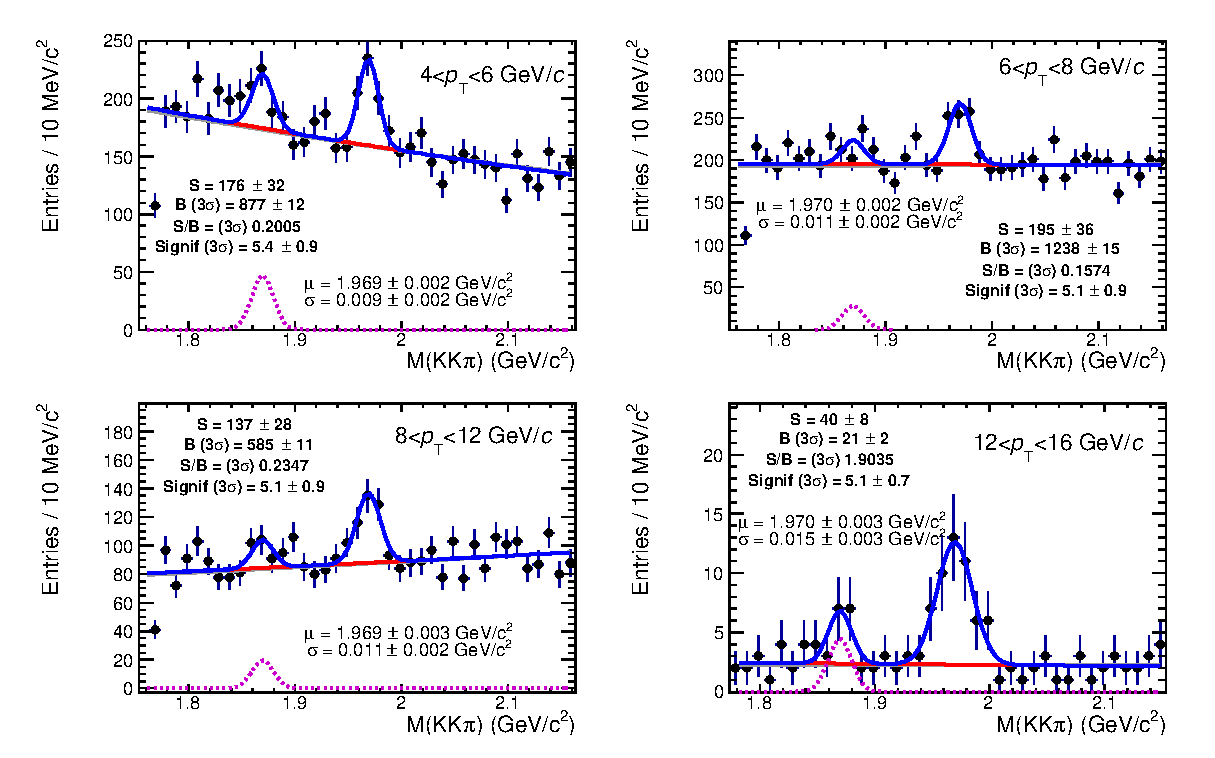
\includegraphics[width=.9\textwidth]{FigCap5/DsMassHistos_010.eps}
\end{center}
 \caption{Fits to the invariant-mass distribution of $\DstoKKpi$ candidates (and charge conjugates) in the four $\pt$ intervals between $4 < \pt < 16 \, \Gevc$ in the 0-10\% centrality class. }
 \label{fig:FigInvMassDs_pbpb010} 
\end{figure} 
\begin{figure}[!h]
 \begin{center}
  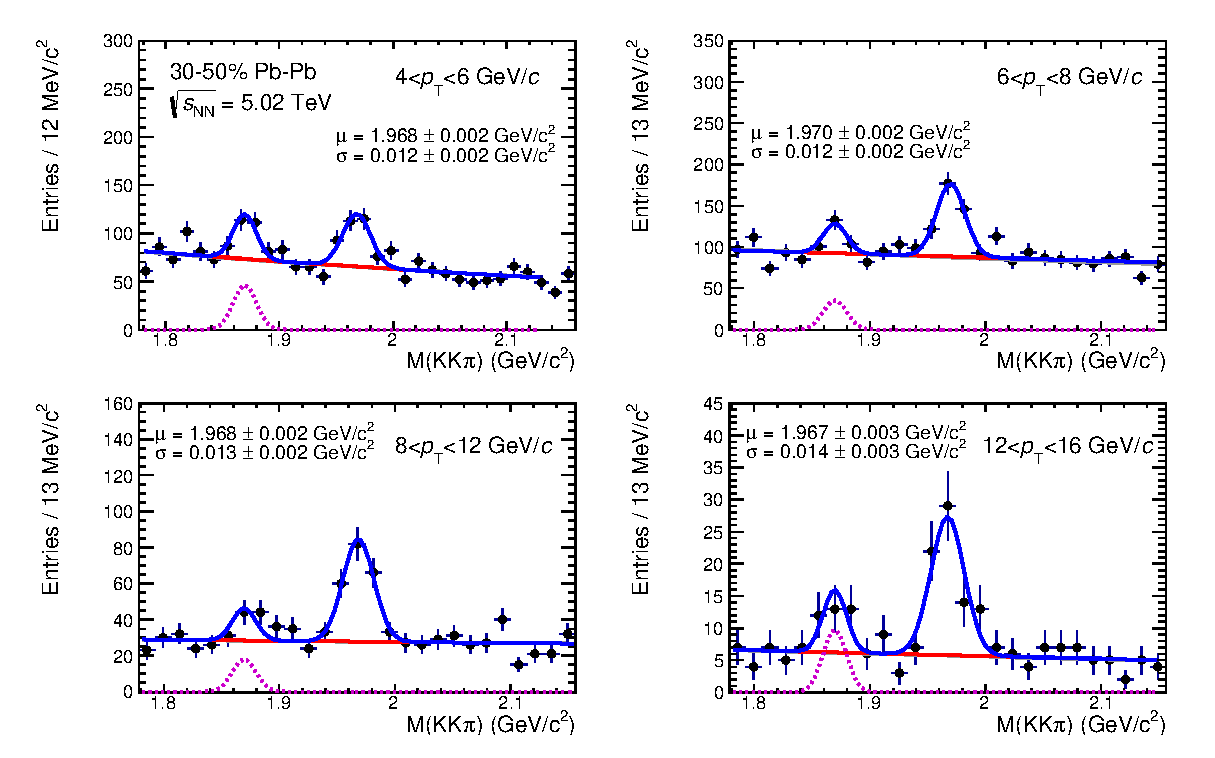
\includegraphics[width=.9\textwidth]{FigCap5/DsMassHistos_3050.eps}
\end{center}
 \caption{Fits to the invariant-mass distribution of $\DstoKKpi$ candidates (and charge conjugates) in the four $\pt$ intervals between $4 < \pt < 16 \, \Gevc$ in the 30-50\% centrality class. }
 \label{fig:FigInvMassDs_pbpb3050} 
\end{figure} 
\begin{figure}[!ht]
 \begin{center}
  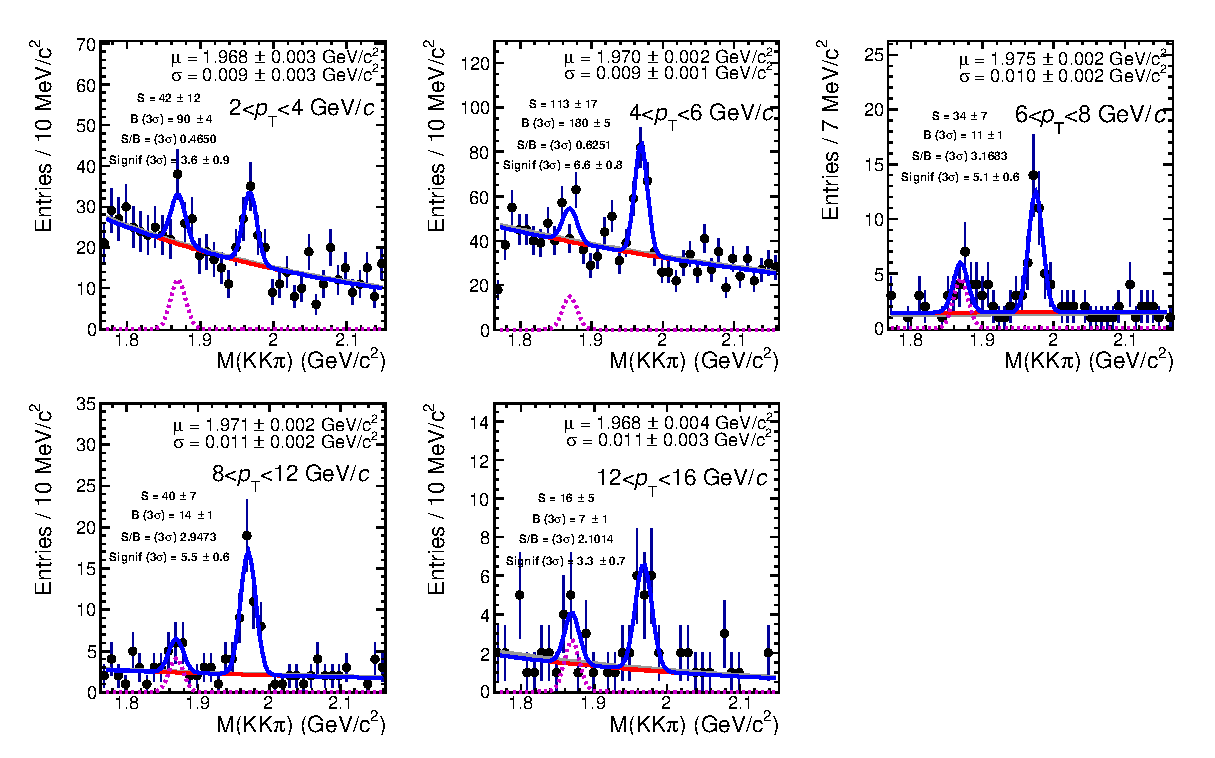
\includegraphics[width=.9\textwidth]{FigCap5/DsMassHistos_6080.eps}
\end{center}
 \caption{Fits to the invariant-mass distribution of $\DstoKKpi$ candidates (and charge conjugates) in the five $\pt$ intervals between $2 < \pt < 16 \, \Gevc$ in the 60-80\% centrality class. }
 \label{fig:FigInvMassDs_pbpb6080} 
\end{figure} 
 

\begin{figure}[!ht]
 \begin{center}
  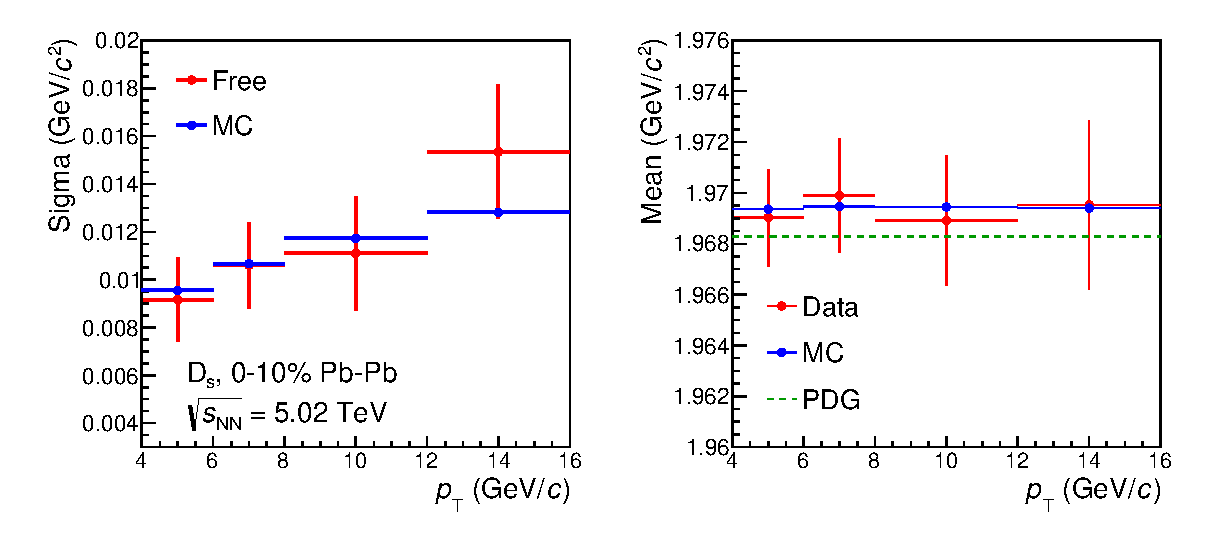
\includegraphics[width=15cm]{./FigCap5/DsMeanSigma_DataMC_010.eps}
  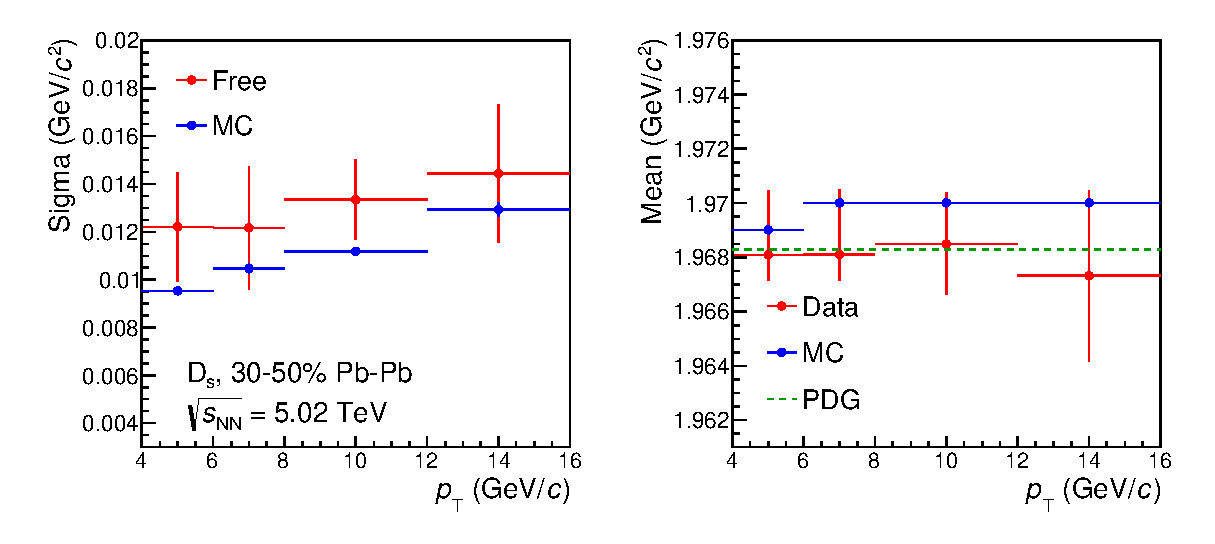
\includegraphics[width=15cm]{./FigCap5/DsMeanSigma_DataMC_3050.eps}
  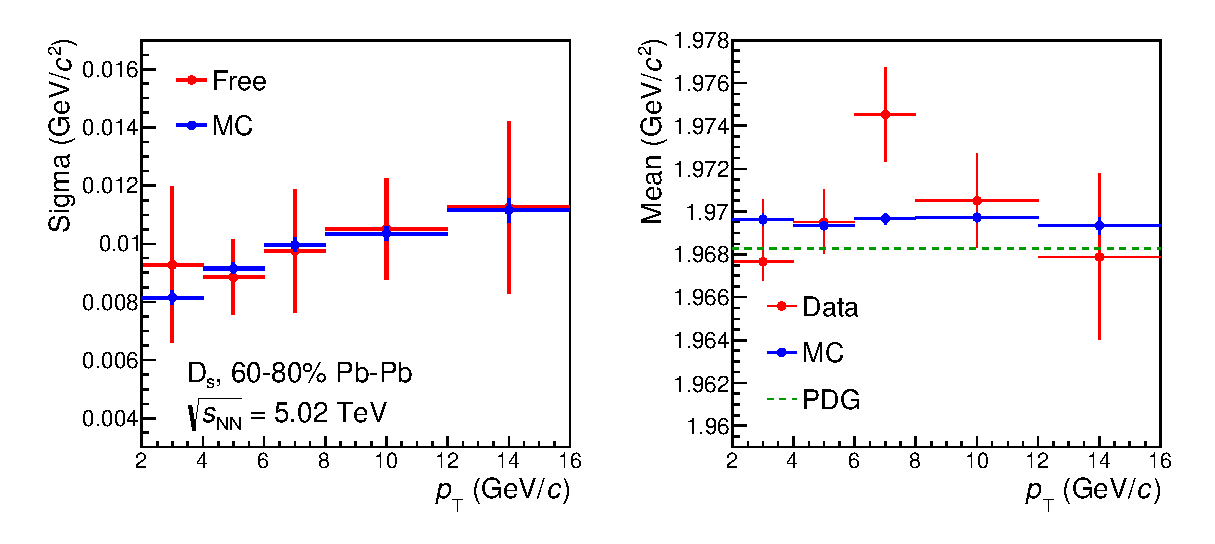
\includegraphics[width=15cm]{./FigCap5/DsMeanSigma_DataMC_6080.eps}
 \end{center}
 \caption{Gaussian width (left) and mean (right) of the $\Ds$ signal peak and as a function of $\pt$: values in data (red) are compared to values in MC (blue). For the peak position, also the PDG value of $\Dsplus$ meson mass (green) is shown. }
 \label{fig:MCsigmacheckDs} 
\end{figure} 


 \begin{table}[!h]
 \begin{center}
  \begin{tabular}{|c|c|c|c|c|c|c|}
\hline
\multirow{2}{*}{$\pt$ bin (GeV$/c$)}& \multicolumn{2}{c|}{0-10$\%$} & \multicolumn{2}{c|}{30-50$\%$} & \multicolumn{2}{c|}{60-80$\%$} \\
\cline{2-7}
& raw yield & S/B & raw yield & S/B & raw yield & S/B \\
\hline
\hline
[2,4] & -  & - & -  & - & 42 $\pm$ 12 & 0.47 \\
\hline
[4,6] &  175 $\pm$ 32  & 0.20 & 141 $\pm$ 26  & 0.35 & 113 $\pm$ 17 & 0.63\\
\hline
[6,8] &  195 $\pm$ 36  & 0.16 & 162 $\pm$ 30 & 0.28 & 33 $\pm$ 7 & 3.08 \\
\hline
[8,12] & 137 $\pm$ 28 & 0.23 & 137 $\pm$ 18 & 0.86 & 40 $\pm$ 7 & 2.95 \\
\hline
[12,16] & 40 $\pm$ 8  & 1.90 & 56 $\pm$ 11 & 1.57 & 16 $\pm$ 5 & 2.10 \\
\hline
  \end{tabular}
 \caption{$\Ds$ raw yields (sum of particles and anti-particles) and signal over background per $\pt$ interval for the three analysed centrality classes.}
  \label{tab:signalDs_010_3050_6080}
\end{center}
\end{table} 

\subsection{Corrections}
\label{sec:CorrectionsAA}
The $\Dspm$-meson raw yields were corrected in order to obtain the
$\pt$-differential yields of prompt $\Dsplus$ mesons: 
\begin{equation}
  \label{eq:dNdpt}
  \left.\frac{{\rm d} N^{\Dsplus}}{{\rm d}\pt}\right|_{|y|<0.5}=
  \frac{\left.f_{\rm prompt}(\pt)\cdot \frac{1}{2} N_{\rm raw}^{\rm
        \Dspm}(\pt)\right|_{|y|<y_{\rm fid}}}{\Delta\pt \cdot
   C_{\Delta y} \cdot ({\rm Acc}\times\epsilon)_{\rm prompt}(\pt)
    \cdot{\rm BR} \cdot N_{\rm events}}\,.
\end{equation}
The difference with respect to Eq.~\ref{sec:corrPP} is that the raw yields $N_{\rm raw}^{\rm \Dspm}$ were divided
by the number of events ($N_{\rm events}$) instead of the integrated luminosity.
The raw yields $N_{\rm raw}^{\rm \Dspm}$ were also divided by 
a factor of two to obtain the charge-averaged (particle and antiparticle) 
yields. To correct for the contribution of feed-down from B-meson decays,
 the raw yields were multiplied by the fraction of promptly produced D 
 mesons, $f_{\rm prompt}$. Furthermore, they were divided by the product 
 of prompt D-meson acceptance and efficiency 
 $({\rm Acc}\times\epsilon)_{\rm prompt}$, by the branching ratio {\rm BR} 
 of the decay channel and by the transverse momentum interval width 
 ($\Delta \pt$). The rapidity acceptance 
 correction factor $C_{\Delta y}= 2 y_{\rm fid}(\pt)$ was calculated as described in Sec.~\ref{sec:corrPP}.

The correction for acceptance and efficiency $({\rm Acc}\times\epsilon)_{\rm prompt}$ 
was determined using Monte Carlo simulations with a detailed description 
of the detector and its response, based on the GEANT3 transport 
package~\cite{Brun:1994aa}. 
The underlying Pb--Pb events at $\sqrtsNN = 5.02$~TeV were simulated 
using the HIJING v1.383 generator~\cite{Wang:1991hta} and D-meson 
signals were added with the PYTHIA v6.421 generator~\cite{Sjostrand:2006za} 
with Perugia-2011 tune. Each simulated PYTHIA event contained a 
$\rm c\overline c$ or $\rm b\overline b$ pair. Only the particles originating from the 
fragmentation of $c$ ($\bar{c}$) and $b$ ($\bar{b}$) quarks were
injected in the event. D mesons were forced to 
decay into the hadronic channels of interest for the analysis. 
\begin{figure}[!b]
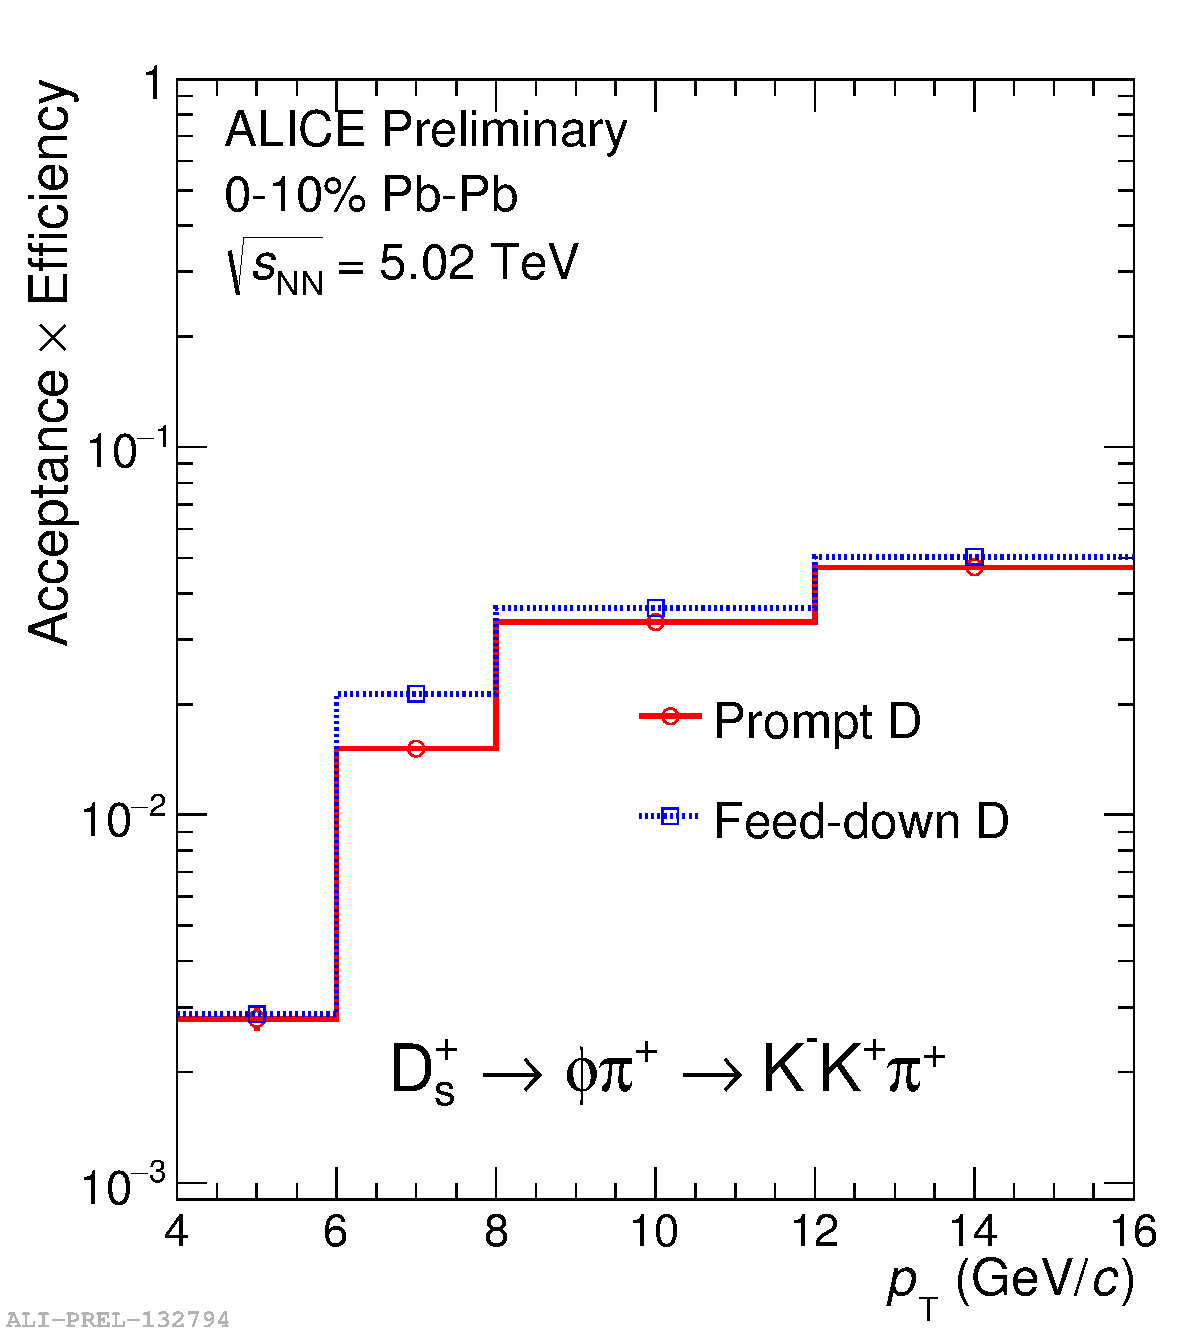
\includegraphics[width=.49\textwidth]{FigCap5/AccEff_Ds_010.pdf}
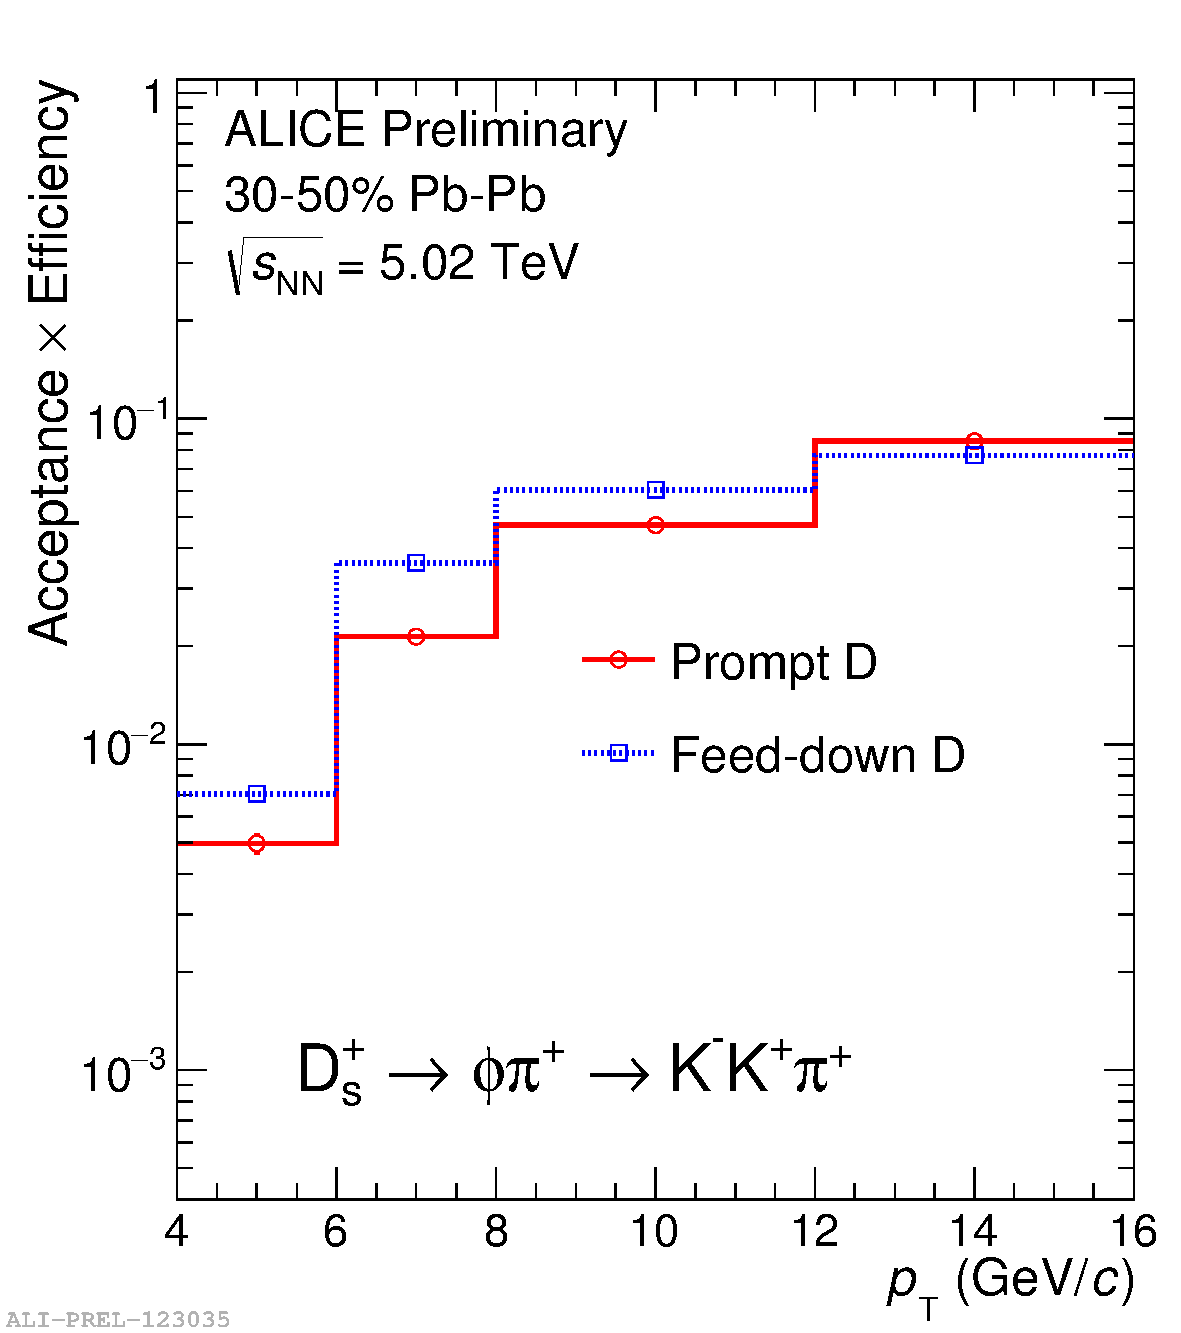
\includegraphics[width=.49\textwidth]{FigCap5/AccEff_Ds_3050.pdf}
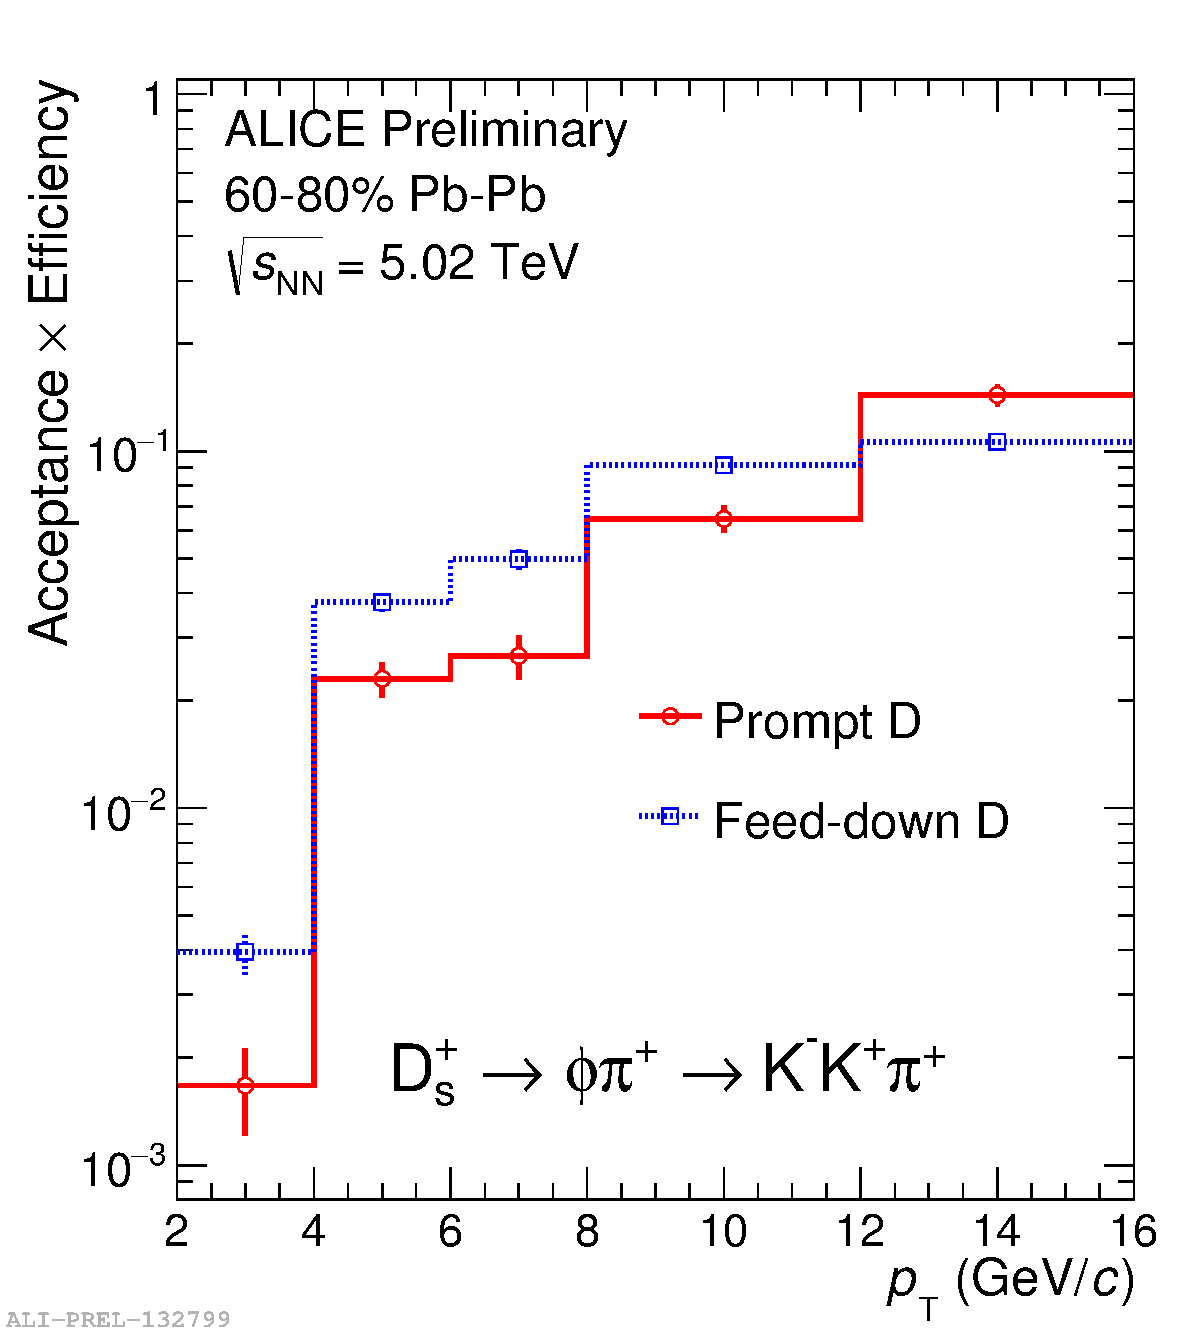
\includegraphics[width=.49\textwidth]{FigCap5/AccEff_Ds_6080.pdf}
\caption{Acceptance times efficiency for $\Ds$ mesons in the three centrality classes, as a function of $\pt$, for prompt (red) and feed-down (blue) components.}
\label{fig:DsAccEff}
\end{figure}
The number of $c\bar{c}$ pairs added to each Pb-Pb 
event was adjusted according to the Pb-Pb collision centrality. 
The efficiencies were evaluated in a centrality class 
corresponding to the one used in 
data in terms of charged particle 
multiplicity in the mid-rapidity region, hence of the detector occupancy.
In the most central event class, the generated $\pt$ distribution 
of $\Ds$ mesons was tuned utilising a re-weighting procedure in order to match the 
shape measured for \mbox{$\rm D^0$ mesons} in finer 
$\pt$ intervals. In the other two centrality classes, 
where an analysis of $\Dzero$-meson yield in finer $\pt$ intervals was not possible, 
the simulated $\Ds$-meson $\pt$ distribution was weighted 
to match the shape given by fixed-order next-to-leading-log 
perturbative QCD calculations (FONLL)~\cite{Cacciari:1998it,Cacciari:2001td} 
multiplied by the $\RAA(\pt)$ of D mesons computed 
using the BAMPS model for semi-central 
collisions~\cite{Uphoff:2011ad,Fochler:2011en,Uphoff:2012gb}.
Fig.~\ref{fig:DsAccEff} shows the acceptance-times-efficiency 
corrections for prompt and feed-down $\Ds$ mesons in the three
centrality classes.
Some of the topological selections tend to reject 
less feed-down due to the larger 
decay length with respect to the prompt D mesons. 
Other topological cuts, like the one on the normalised 
track-impact parameter residual, are more effective
in rejecting the feed-down component, allowing higher 
prompt efficiencies at high $\pt$.
The reconstruction and selection efficiencies for prompt and feed-down
$\Ds$ mesons in Pb-Pb collisions are smaller than the results in pp 
collisions up to a factor of 3 as a consequence of
the tighter topological selection applied. \\

\begin{figure}[!htb]
 \begin{center}
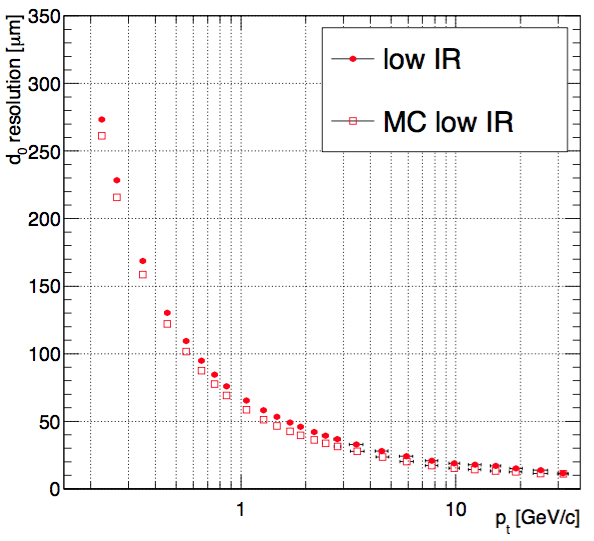
\includegraphics[width=.49\textwidth]{./FigCap5/d0Reso.png}
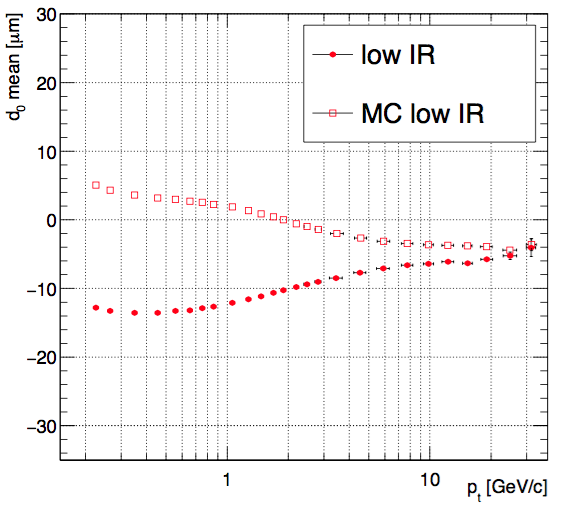
\includegraphics[width=.49\textwidth]{./FigCap5/d0Mean.png}
\end{center}
 \caption{Impact parameter resolution in the transverse plane (left) and mean value (right) in 2015 Pb-Pb data taking at $\sNN = 5.02$ TeV for low interaction rate runs compared to Monte Carlo simulations.}
 \label{fig:d0}
\end{figure}



Fig.~\ref{fig:d0} shows the resolution of the impact parameter of reconstructed tracks 
in the transverse plane ($d_{\rm 0}^{\rm xy}$), for low interaction rate runs in data and in simulations.
The values of the resolution are obtained via a fit to the distributions of $d_{\rm 0}^{\rm xy}$ 
of charged tracks, in the different $\pt$ intervals. The histograms are fitted by a function consisting of a sum
of a Gaussian, to describe the $d_{\rm 0}^{\rm xy}$ of primary particles, and an exponential
function for the tails of the distribution, whose main contributors are secondary tracks,
that have larger impact parameter values. The position of the Gaussian function
should be compatible to 0 if no biases are present, while the width is
the resolution on the impact parameter values, which depends on the transverse momentum of the tracks.
The values of the impact parameter resolution in data are not fully reproduced
in the simulations (see Fig.~\ref{fig:d0}, left panel).
Furthermore, the impact parameter distribution is shifted to negative 
values by up to 10-15 micron at low $\pt$ and 
decreasing to 5-10 micron at high $\pt$. The shift 
depends on the azimuthal angle and is not described 
in the MC (Fig.~\ref{fig:d0}, right panel). 
The information on detector alignment used in the reconstruction of the Pb-Pb sample dates back to early 2015.
The observed bias in the simulation has a dependence on the B field polarity and on the time.
This suggests that the bias originates from a residual misalignment in the simulation
that slightly vary as a function of time. Furthermore, a minor part of the shift is caused
by the presence of three SPD modules which were not included in the detector alignment.
In order to reduce possible systematic effects arising from these discrepancies
between data and simulations, a tuning procedure of the Monte Carlo output
was developed.
%Current hypothesis is that part of the shift 
%is due to the presence of SPD modules that were not 
%included in the detector alignment (because they were
% included only afterwards in the data taking). 
 The impact parameter resolution measured in data 
 was reproduced in MC by applying to the tracks of the simulated sample a scaling of 
the residuals ${\rm d}_0^{\rm true}-{\rm d}_0^{\rm reco}$ 
 according to the data-to-MC ratio of the impact parameter 
 resolutions. A shift of d$_0^{\rm reco}$ was also applied to correct for the different bias in MC and in data.
 The covariance matrix of the track was also
 updated after the corrections, in order not to introduce biases at the level
 of topological variables based on standardised quantities such as the normalised decay length. \\
% These corrections were verified to have small impact on D-meson efficiencies.\\
 


The $f_{\rm prompt}$ factor, which corrects for the contribution of 
D mesons from B-meson decays in the measured raw yield 
in each $\pt$ interval, was obtained following the procedure described in Sec~\ref{sec:ppFprompt}. 
The expression for $f_{\rm prompt}$ reads:
\begin{equation}
\label{eq:fprAA}
\begin{split}
f_{\mathrm{prompt}} = \, & 1- \frac{N^{\text{D~feed-down}}_{\mathrm{raw}}}{N^{\mathrm{D}}_{\mathrm{raw}}}=\\
& 1- \RAA ^{\rm feed-down} \cdot  \langle \TAA \rangle \left (\frac{\rm d^2 \sigma}{\mathrm d\pt \mathrm d y} \right)^{\rm FONLL}_{\text{feed-down}} \cdot  \frac{(\mathrm{Acc} \times \epsilon)_\text{feed-down} \cdot \Delta y \Delta \pt \cdot \mathrm{BR} \cdot L_{\rm int}}{N^{\rm D +\overline{D},raw}/2}\,.
\end{split}
\end{equation}
The difference with respect to Eq.~\ref{eq:fpr} is that the beauty-hadron 
production cross section from FONLL pQCD
calculations in pp collisions at $\sqrt{s}=5.02~\tev$~\cite{Cacciari:2012ny}
is multiplied by the average nuclear overlap function $\langle \TAA \rangle$ of the corresponding centrality class. 
In addition, a hypothesis on the nuclear 
modification factor of feed-down $\Ds$ mesons, $\RAA^{\textnormal{feed-down}}$, was 
introduced to account for the different modification of beauty and charm 
production in Pb-Pb collisions. The resulting sample of 
feed-down $\Ds$ mesons is composed of two 
contributions: about 50\% of the feed-down originates from 
B$^0_{\rm s}$-meson decays, while the remaining 50\% comes from decays of 
non-strange B mesons (B$^0$ and B$^+$) (see Fig.~\ref{fig:DsParentsAndFDunc} left).
To determine the central value of $f_{\rm prompt}$ in the 0-10\% 
and 30-50\% centrality classes, it was assumed that the 
nuclear modification factors of feed-down and prompt $\Ds$ mesons were equal 
($\RAA^{\textnormal{feed-down}}=\RAA^{\rm prompt}$). 
The resulting feed-down contribution is about 10\%, depending on the
$\pt$ interval, as it is shown in Fig.~\ref{fig:promptAA}
\begin{figure}[!htb]
 \begin{center}
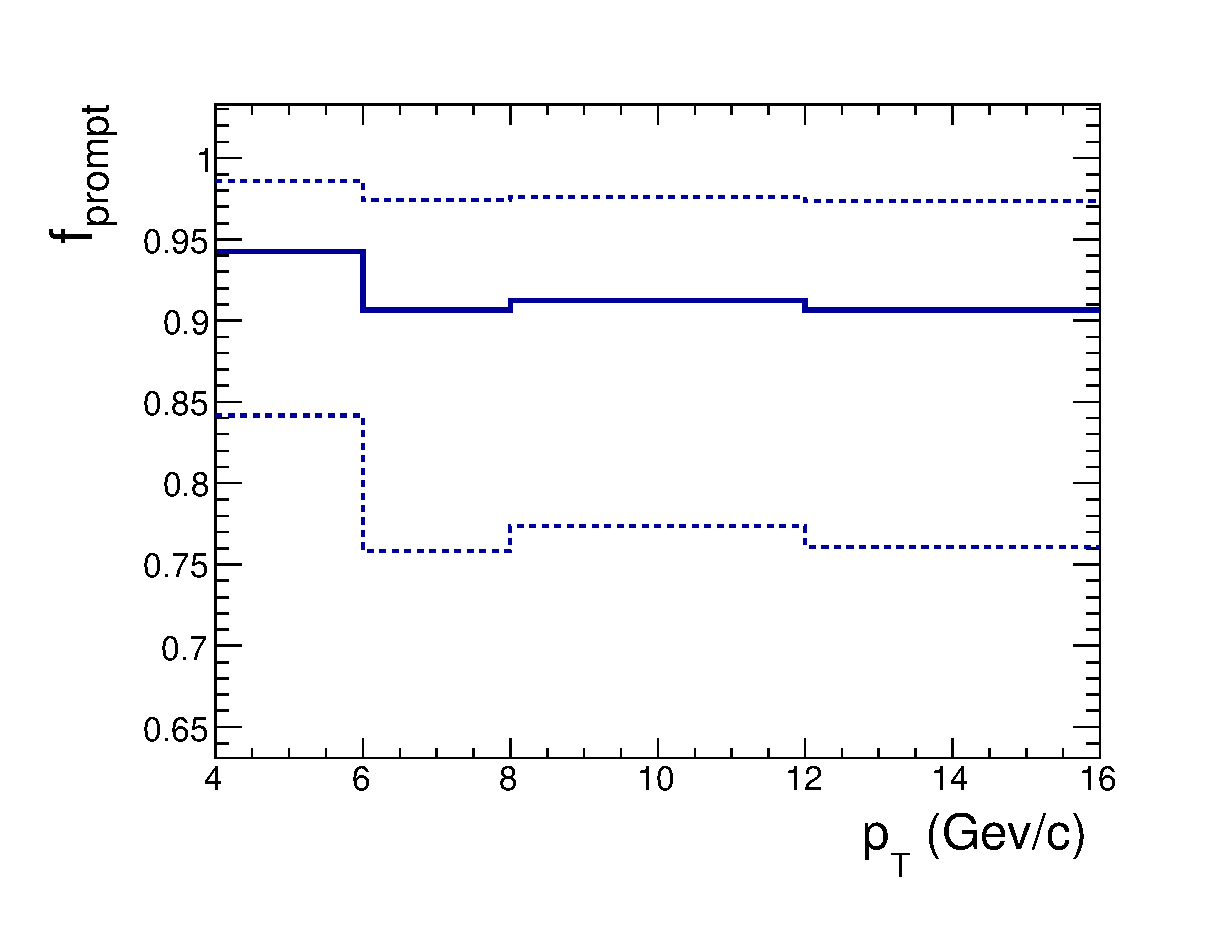
\includegraphics[width=.54\textwidth]{./FigCap5/fprompt010.eps}
\end{center}
 \caption{Prompt fraction of $\Ds$ yield in the 0-10\% centrality class as a function of $\pt$.}
 \label{fig:promptAA}
\end{figure}
To determine the systematic uncertainty the hypothesis
was varied in the range $1/3<\RAA^{\textnormal{feed-down}}/\RAA^{\rm prompt}<3$, as 
discussed in detail in Section~\ref{sec:systematics}.
It should be noted that the central value and the range of the hypothesis
on $\RAA^{\textnormal{feed-down}}/\RAA^{\rm prompt}$ differ from those used for
non-strange D mesons in Refs.~\cite{ALICE-PUBLIC-2017-003,Adam:2015sza}. The 
central hypothesis of $\RAA^{\textnormal{feed-down}}/\RAA^{\rm prompt}$ for non-strange
D mesons is in fact set at 2  due to the comparison of the $\RAA$ of prompt D mesons at 
$\sNN = 2.76$ TeV~\cite{Adam:2015nna} with that of J/$\psi$ from B-meson decays~\cite{Khachatryan:2016ypw} 
measured in the CMS experiment (see Sec.~\ref{sec:resAAcap2}), that indicates that charmed hadrons 
with $\pt > 8 \, \Gevc$ are more suppressed than beauty hadrons in semi-peripheral and central
Pb-Pb collisions relative to binary scaled pp collisions. The hypothesis for $\Ds$ meson
accounts for the recombination in the charm and beauty sectors.
The contribution of coalescence of charm quarks should enhance the $\RAA$ of
$\Ds$ with respect to that of non-strange D mesons. If recombination does not occur
for beauty quarks, the suppression of $\Ds$ could result similar to that of  B$^0$, B$^+$ and B$^0_{\rm s}$
mesons. If, on the other hand, recombination plays a role for beauty,
the hypothesis on $\RAA^{\textnormal{feed-down}}$ accounts for a possible enhancement 
of the ratio of B$^0_{\rm s}$ over non-strange B mesons~\cite{TAMULHC}
and for the large fraction of feed-down $\Ds$ mesons originating from non-strange B-meson decays.
For the peripheral class 60--80\%, in which the medium effects are milder, 
also the difference between charm and beauty mesons is assumed to be 
reduced: the value $\RAA^{\textnormal{feed-down}}=1.3\cdot\RAA^{\rm prompt}$ 
was used for all D-meson species and the range of the hypothesis to estimate the
uncertainty was reduced. 

\begin{figure}[!htb]
 \begin{center}
\includegraphics[width=15.cm]{./FigCap5/MT_Pt812.png}
\end{center}
 \caption{Output of multiple-trial fits to $\Ds$ invariant-mass distributions in the $\pt$ intervals 8-12 $\Gevc$, for the 0-10$\%$ centrality class.}
 \label{fig:multitrial_Ds_010}
\end{figure}


\section{Systematic uncertainty on corrected d$N$/d$\pt$}
\label{sec:systematics}
Most of the sources of systematic uncertainty considered for the analysis 
of the corrected yields and the methods used to estimate them were already described in Sec.~\ref{sec:systPP}. 
Hence in the next sections we will concentrate on the differences with respect to the 
pp analysis. Table~\ref{tab:sysunc_yieldtable} summarises the 
assigned systematic uncertainties in the three analysed centrality classes.

\subsection{Yield extraction systematics}
\label{sec:YieldExsystAA}
The estimate of the systematic uncertainty on the yield extraction
was based on the multiple-trial fit approach described in Sec.~\ref{sec:RawYieldSyst}
(it is the first approach of the two presented there).
Fig.~\ref{fig:multitrial_Ds_010} shows an example of the multiple trial fit procedure on the invariant-mass
distribution in the interval $8 < \pt < 12 \, \Gevc$, for the 0-10\% centrality class.
The panels of the figure show, starting from top left plot:
(i) the raw yield distributions from the multiple trials,
with the histograms obtained via fit and bin counting shown
in different colours; (ii) the distribution of raw yields from multiple 
trials, distinguishing the cases in which the Gaussian width of the signal function was left as free parameter 
in the fit, or was fixed to its MC value or fixed to MC value +15\% (where
15\% is the average underestimate of the width value in MC with respect to data in some
$\pt$ intervals); 
(iii) the distribution of the reduced $\chi^{2}$ of the fits; 
(iv) the Gaussian width of the peak as a function of the trial 
number; (v) the raw yield distribution as a 
function of the trial number; (vi) a panel reporting the Gaussian RMS value (used as
estimator of the systematic uncertainty) of the yield distribution
in two cases: considering the yields extracted from the fits with 
the Gaussian sigma left as free parameter in the fit or fixed to its MC values
as well as those obtained considering the cases with sigma free, fixed to MC and fixed to 
MC +15\%. The systematic uncertainty was estimated from the RMS
of the first distribution. For those $\pt$ intervals where the value of the width in 
simulation underestimates that in data, it was verified that
the RMS of the second distribution was in agreement with the assigned value for the
systematic uncertainty. 
It was also verified that the difference between the mean values of the yield distributions from fit
and from bin counting methods was contained within the RMS value quoted 
as systematic uncertainty.
The final assigned uncertainties range from 5\% to 10\% depending on $\pt$ and
centrality class and are reported in Tab.~\ref{tab:sysunc_yieldtable}. 




\begin{figure}[!h]
 \begin{center}
   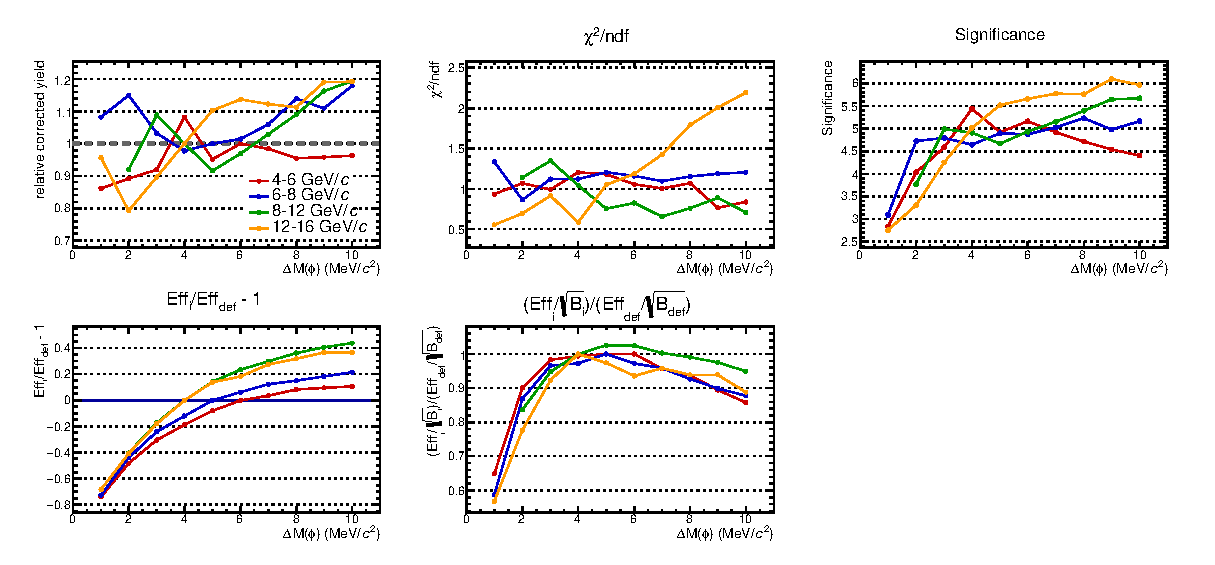
\includegraphics[angle=0, width=15cm]{./FigCap5/cutbycut_invm_010.eps}
 \end{center}
 \caption{Distribution of the $\Ds$ corrected yields in the 0-10\% centrality class, obtained varying the selection on the invariant mass of the reconstructed $K^+K^-$ pair (top left panel). The other panels report the values of reduced $\chi^2$, significance, selection efficiency, selection efficiency divided by the to square root of the background counts.}
 \label{fig:DeltaMDsCutVar_010} 
\end{figure}
\begin{figure}[!h]
 \begin{center}
   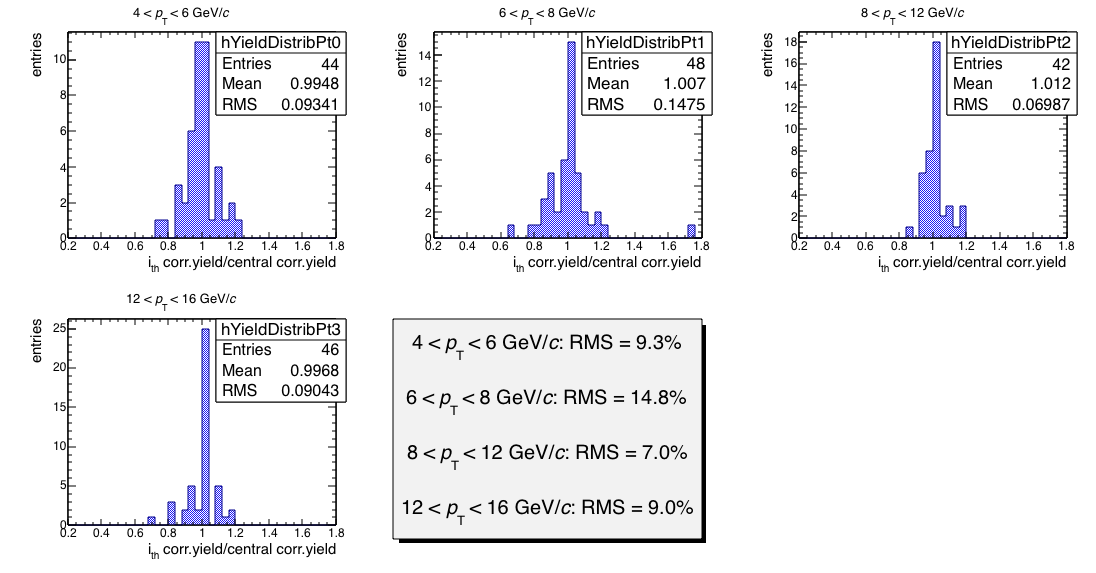
\includegraphics[angle=0, width=15cm]{./FigCap5/FinalSyst_010.png}
 \end{center}
 \caption{Distribution of $\Ds$ corrected yields in the 0-10\% centrality class, from the variation of the selection criteria with respect to the default value.}
 \label{fig:DsCutVar_010} 
\end{figure}

\subsection{Selection efficiency}
\label{sec:CutVarsystAA}
The systematic uncertainty on the efficiency of the $\Ds$ selection was studied
via cut variation procedures, similarly to what done for pp collisions (see Sec.~\ref{sec:CutVariation}).
A systematic scan from looser to tighter cuts was done on a variable-per-variable 
basis, extracting the raw yields, correcting them with the corresponding efficiency, 
comparing the corrected yields to those obtained 
with a reference set of cuts and looking for possible trends/biases of 
the corrected yield as a function of the cut strength.
The study was done using as reference set of cuts the one used 
to provide the central values of the yields. A selection
on the basis of the $\chi^2/ndf$ ($<2.5$) of the invariant-mass fits and the statistical significance ($>2$)
of the signal was applied to reject the sets of cuts that were not showing a robust 
determination of the raw yield.  
An example of the scan performed on the cut on the
reconstructed K$^+$K$^-$ invariant-mass pair is shown in Fig.~\ref{fig:DeltaMDsCutVar_010}.
The top-left panel shows the ratios of the corrected yields 
(at a specific cut value) to that obtained with the default
cut, in different colours for the different $\pt$ intervals.
Some systematic deviations from unity of this ratio are visible when the selection
on this variable is released with respect to the default cut ($\Delta M < $ 4-6 GeV/$c^2$ depending
on the $\pt$ interval). 
This behaviour could be due to a systematic effect originating, e.g., from a 
different $\pt$ resolutions in data and in MC, as well as to a less-reliable extraction of 
the raw yield in the cases of low S/B ratios with loose selections.
The statistical significance (top-right panel) of the signal and
the reduced $\chi^2$ (middle-top panel) as a function of the cut value were also considered.
The relative variation of the selection
efficiencies with respect to that with default set of cuts is shown in the bottom-left panel.
Finally, in the bottom-middle panel the ratio of the selection efficiency to the square root of 
background counts in the interval within $3\sigma$ around the peak complements 
the information from the statistical significance,
and it is less affected by possible fluctuations of the signal.
Since the values of the reduced $\chi^2$ and of the statistical significance do
not allow to reject any set of cuts shown in Fig.~\ref{fig:DeltaMDsCutVar_010},
the corrected yields from this study were collected, for each $\pt$ interval,
into inclusive distributions. The RMS values of these distributions provide an estimate for the systematic uncertainty.
Fig.~\ref{fig:DsCutVar_010} shows an example of these final distributions 
for the 0-10\% centrality class, in the four analysed $\pt$ intervals. 
The values of the RMS of the Gaussian distributions are reported
in the last panel.

\subsection{PID selection efficiency}
\label{sec:PIDsystAA}
To estimate the systematic uncertainty due to PID efficiency,
two particle identification selections (a tighter one, discussed in Sec.~\ref{Sec:PID}, and a 
looser, in Sec.~\ref{sec:PIDsystPP}) were compared. Fig.~\ref{fig:DsPID010} 
shows, as an example for 0-10\% centrality class, the ratio of the corrected yields 
with looser and tighter PID selections. Due to the large error bars, it is difficult to asses
whether the points are affected by a systematic effect
or they are dominated by statistical fluctuations.
For this reason, an alternative approach of a per-track estimate of the PID
systematic was followed. The idea is to select samples of kaon and pion tracks in data and
MC. 

The difference in the efficiencies for a given N$\sigma$ cut (on d$E$/d$x$ or 
time-of-flight signal) in data and MC will
constitute a $\pt$-dependent per-track systematics for each species.

\begin{figure}[!h]
 \centering
 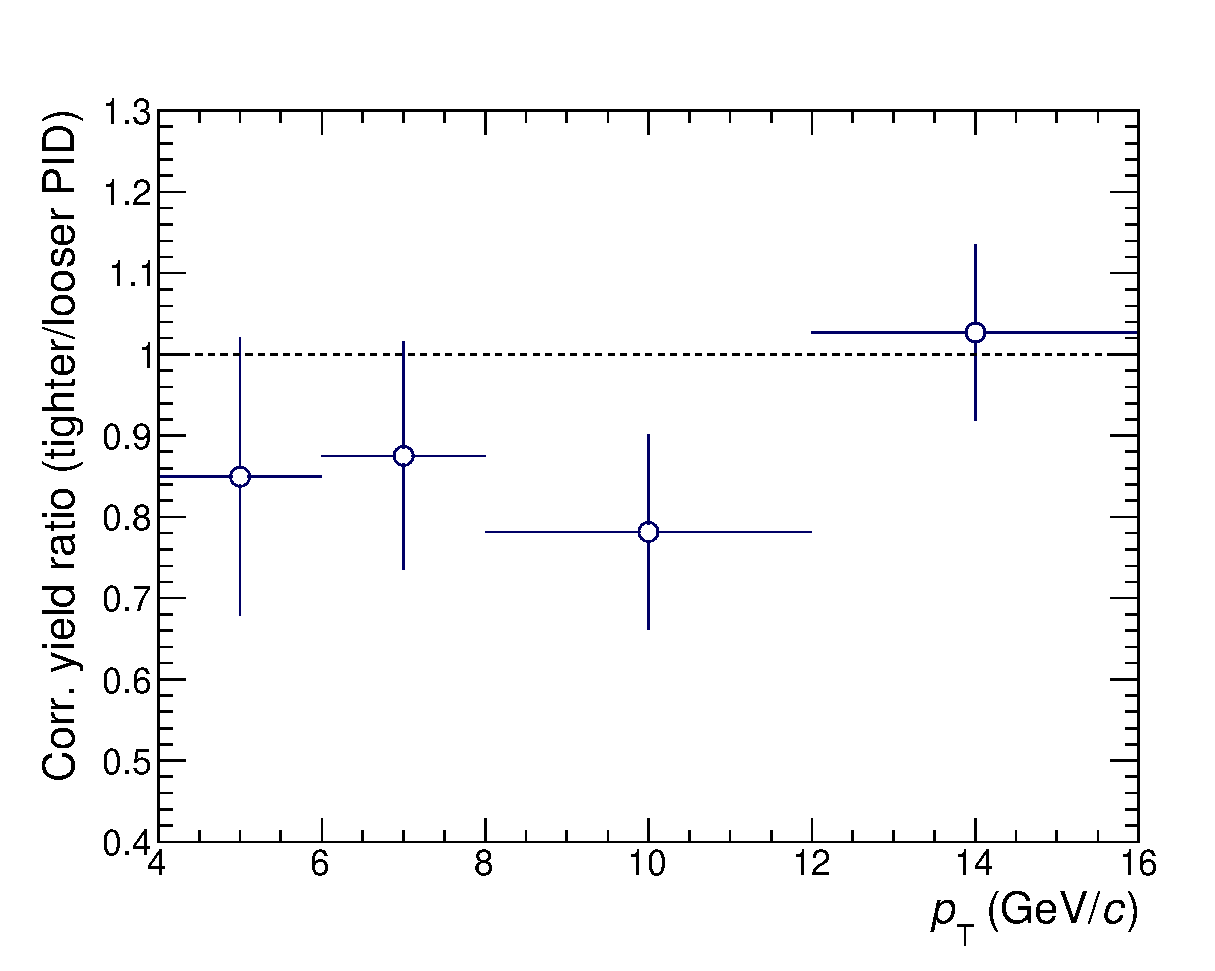
\includegraphics[angle=0, width=7cm]{./FigCap5/PIDsyst_010.eps}
 \caption{Ratio of $\Ds$ corrected yield in 0--10\% centrality class with tighter-to-looser PID selections.}
 \label{fig:DsPID010} 
\end{figure}
Pions from V0 decays were selected using the optimised cuts
used in~\cite{Schuchmann:2102194}. In Fig.~\ref{fig:MCPionsTPC} the Monte Carlo 
N$\sigma$ distributions for the d$E$/d$x$ of pions in TPC are shown for 
different $\pt$ intervals, from 0.2 to 10 $\Gevc$.
The N$\sigma$ distributions of pions (in green) selected utilising the MC truth are compared to the
those of tracks passing the selection as pions from V0 decays 
(in blue). A peak centred at N$\sigma=0$ is the dominant contribution for both
track samples.
A second population (less that 1\% of the total) is visible at the right of the peak at low $\pt$ in the in the N$\sigma$ distribution
of pion candidate tracks from V0 decays. This second population is present
also in the N$\sigma$ distribution obtained from data and shown in
Fig.~\ref{fig:DataPionsTPC} and it is likely a contamination from electrons passing
the pion selection criteria. For this reason, 
only the left side of the peak will be used to study the systematic uncertainty.
A part from this small contamination, we conclude that the utilised selections provide a pure
enough sample of pions. 
In Fig.~\ref{fig:DataPionsTPC}, the N$\sigma$ distributions in data (blue) are compared
to the distributions of true MC pions (green), in the different $\pt$ intervals.  
Finally, the efficiencies of the N$\sigma$ selection in data and in MC are obtained by integrating the corresponding 
distributions (blue and green distributions in Fig.~\ref{fig:DataPionsTPC})
within 1$\sigma$, 2$\sigma$ or 3$\sigma$, and normalising these values to the integral 
of the distributions within 5$\sigma$. It was verified that enlarging the number of $\sigma$ from 5 to 10 at the 
denominator of the efficiency does not affect the final results.
The systematic uncertainty is defined as the difference between the efficiencies 
 of the N$\sigma$ selection in data and in MC.
The same procedure
was carried out with the N$\sigma$ distributions of the time-of-flight signals 
for the pions from V0 decays, to estimate the systematic uncertainty on pion identification with TOF.
To obtain the uncertainty on kaon identification in TPC, a tight cut on the PID 
signal in TOF, requiring the signal to be within N$\sigma < 0.25\sigma$ from the 
kaon expectation value, was applied. 
The black curve in Fig.~\ref{fig:MCKaonsTPC} shows the 
N$\sigma$ distribution for the d$E$/d$x$ of simulated tracks that satisfy this selection.
Contaminations from other particle species are still present and they
are shown in different colours in the same Fig.~\ref{fig:MCKaonsTPC}. 
The black curve was fitted in a region around N$\sigma=0$ with a Gaussian shape 
to extract the kaon contribution. The ranges of the fits are set, for each $\pt$ interval, to exclude 
the regions more affected by contamination from other species.
In Fig.~\ref{fig:DataKaonsTPC}, the distribution of N$\sigma$ for d$E$/d$x$ in data is displayed. 
The Monte Carlo templates for true 
kaons (yellow filled histograms) are superimposed to the data distributions, 
only for visualisation purposes, but they are not used in the fits. The distribution of candidate kaons from the data
was fitted with a Gaussian function in the N$\sigma$-axis range previously tuned on the simulation,
to extract the kaon distribution, in each $\pt$ interval.\\
The values of the data-to-MC ratios
of the efficiencies estimated with this procedure are shown in Fig~\ref{fig:PerTrackPIDsys}, as a function of $\pt$,
for cuts at 1, 2 and 3$\sigma$ on the PID signals. 
Since it is not possible to select a pure sample of kaons to compare the TOF N$\sigma$
distributions, an assumption for the systematic uncertainty on kaon
identification with the TOF is needed. The same uncertainty estimated
for pion identification with TOF is assigned also to kaon identification, based on
the observation that the systematic uncertainties on pion and kaon identification
with the TPC are similar.
The $\pt$-dependent per-track systematics can be propagated to the $\Ds$-meson level, via the kinematics of
the daughter tracks.
This was done by assigning to the $\Ds$ daughter tracks a PID uncertainty 
which depends on their $\pt$. The PID uncertainties of the three daughter tracks
were assumed to be fully correlated and were summed linearly.
The correlation between the $\pt$ of the daughter track and that of $\Ds$ mesons is shown in the
left panel of Fig.~\ref{fig:DsPIDsys}.
The final values of the systematic uncertainties are around 
3\% for the tighter (Sec.~\ref{Sec:PID}) PID selection, utilised for $\Ds$ at low $\pt$ in the 0-10\% and 30-50\% classes and at all $\pt$ in 60-80\% (see Fig.~\ref{fig:DsPIDsys}), and are negligible for the
looser PID selection, used at high $\pt$ in the 0-10\% and 30-50\% classes (Sec.~\ref{sec:PIDsystPP}).

\begin{figure}[!h]
 \centering
 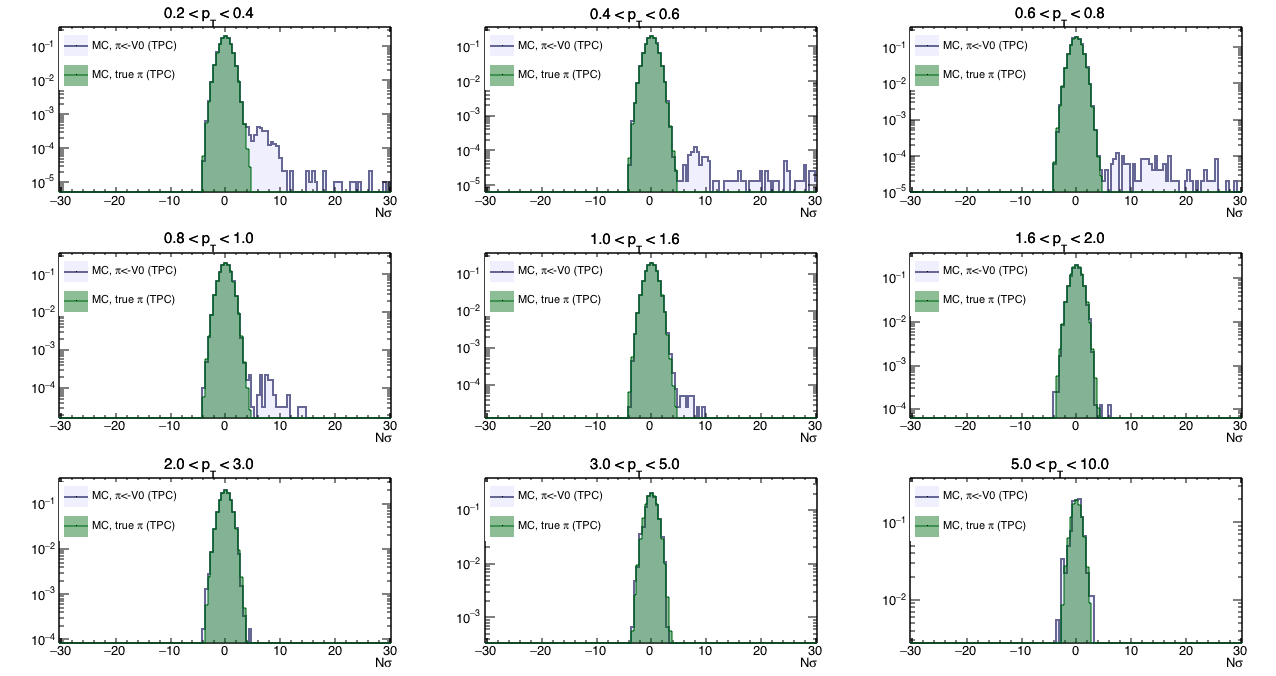
\includegraphics[angle=0, width=15cm]{./FigCap5/PionTPC_MC.png}
 \caption{N$\sigma$ distribution of d$E$/d$x$ signal in TPC for pions in Monte Carlo. In green pions selected by PDG code, in blue tracks passing the selection for pions from V0 decays.}
 \label{fig:MCPionsTPC} 
\end{figure}

\begin{figure}[!h]
 \centering
 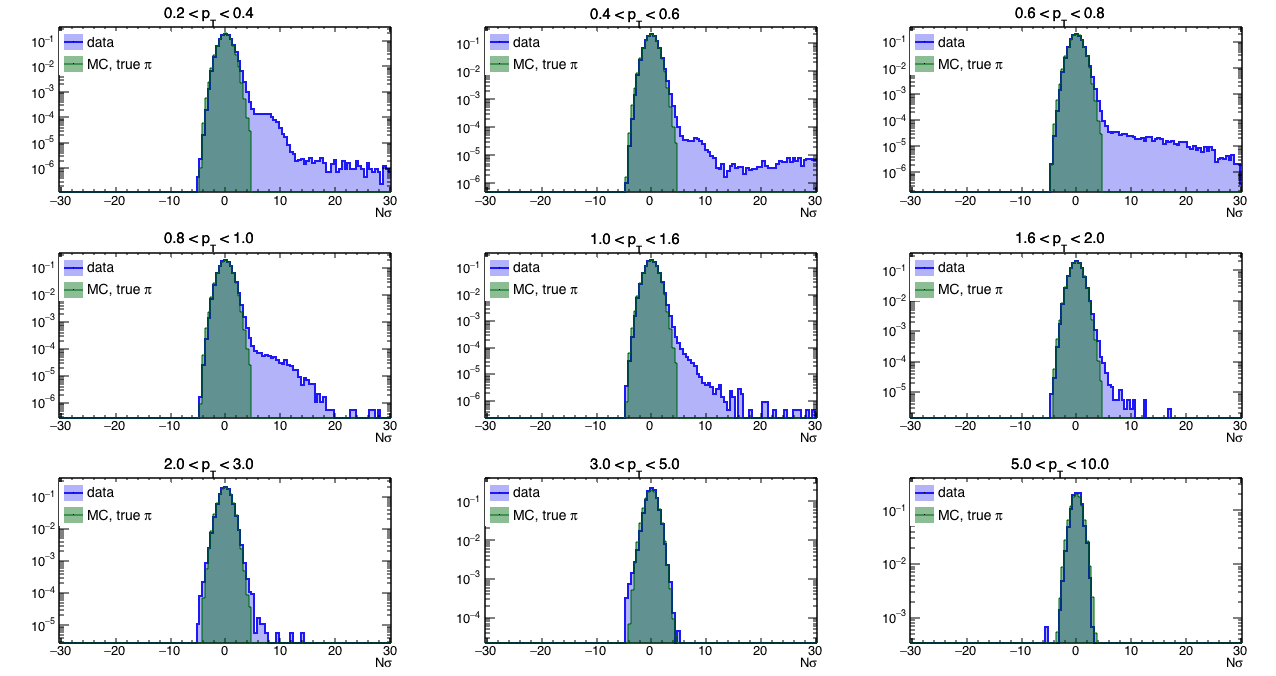
\includegraphics[angle=0, width=15cm]{./FigCap5/PionTPC_DataMC.png}
 \caption{N$\sigma$ distribution of d$E$/d$x$ signal in TPC for pions in data (blue) and Monte Carlo (green)}
 \label{fig:DataPionsTPC} 
\end{figure}

\iffalse
\begin{figure}[!h]
 \centering
 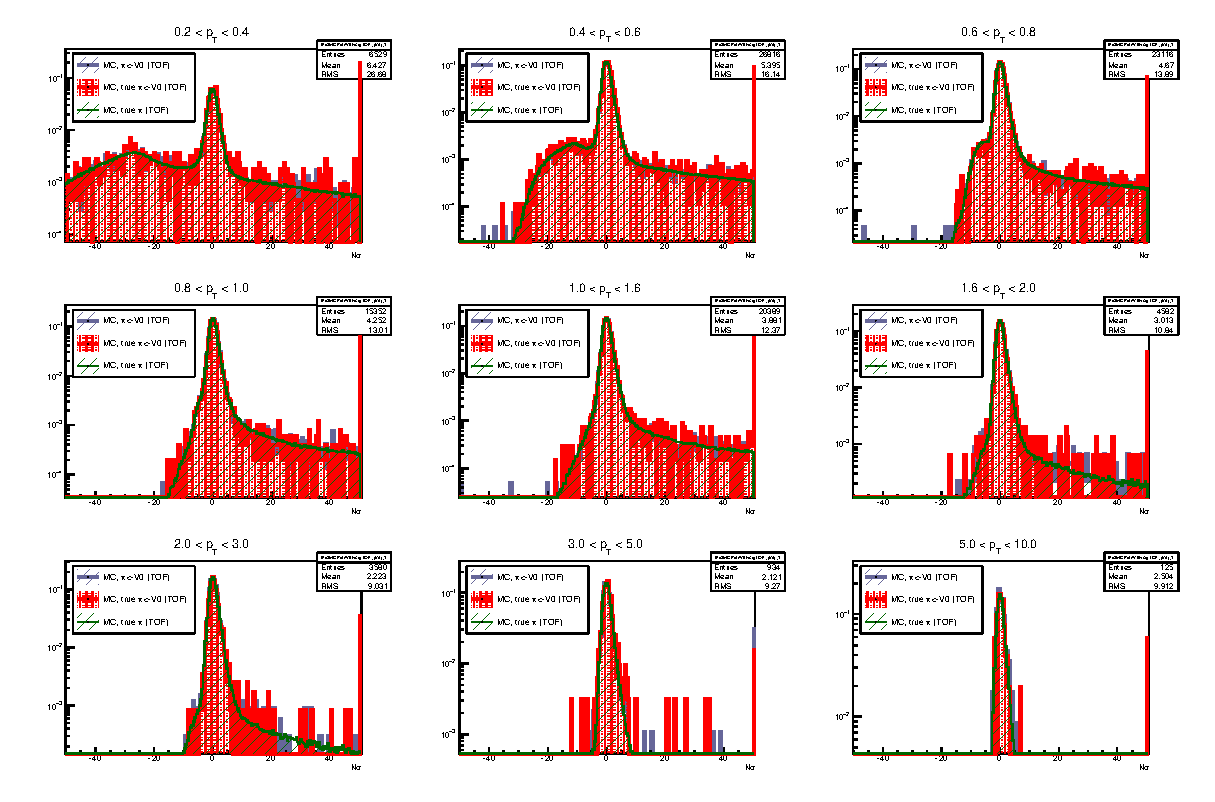
\includegraphics[angle=0, width=13cm]{./FigCap5/MCPionTOF_AllTrueSig.eps}
 \caption{N$\sigma$ distribution of t.o.f. signal in TOF for pion hypothesis in Monte Carlo. In green pions selected by PDG code, in blue and in red pions passing the selection for V0 decays without and with PDG code selection respectively.}
 \label{fig:MCPionsTOF} 
\end{figure}
\fi

\begin{figure}[!h]
 \centering
 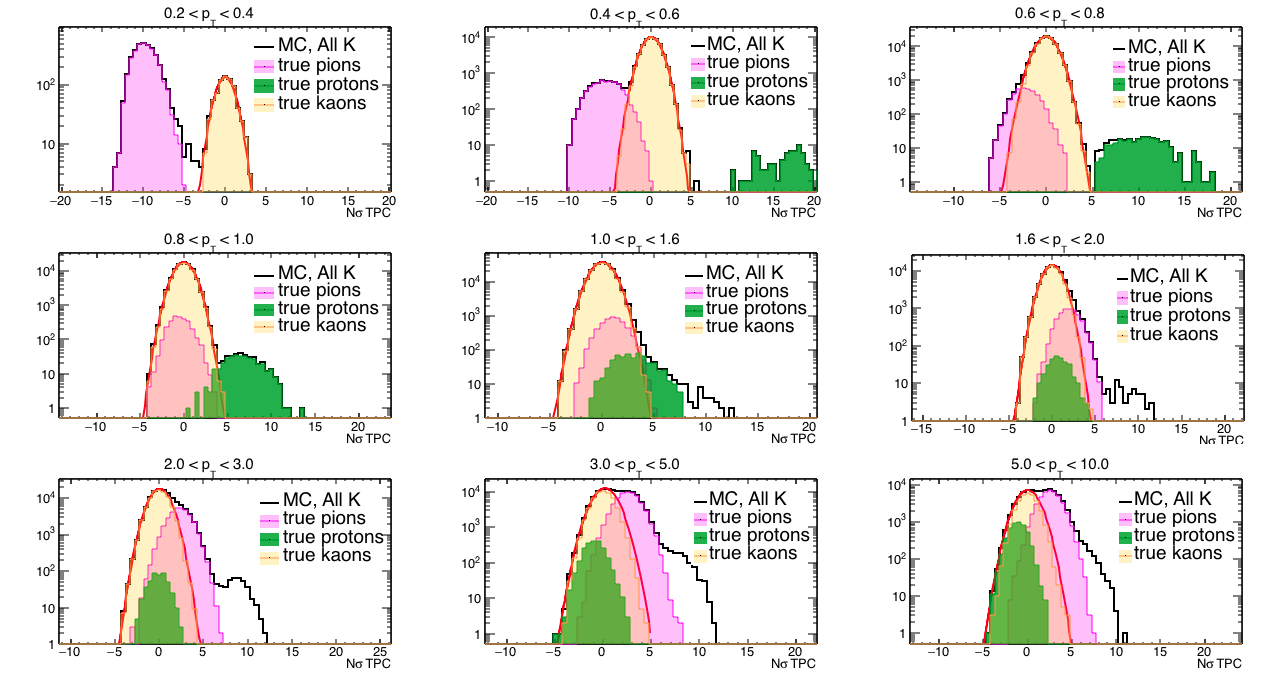
\includegraphics[angle=0, width=15cm]{./FigCap5/KaonTPCFromTOF_MC.png}
 \caption{N$\sigma$ distribution of d$E$/d$x$ signal in TPC for tracks from the Monte Carlo simulation that pass the selections as kaons (black curve). In yellow, contribution from true kaons, in magenta from pions and in green from protons. The fit to extact the kaon component from the inclusive distribution is shown in red.}
 \label{fig:MCKaonsTPC} 
\end{figure}

\begin{figure}[!h]
 \centering
 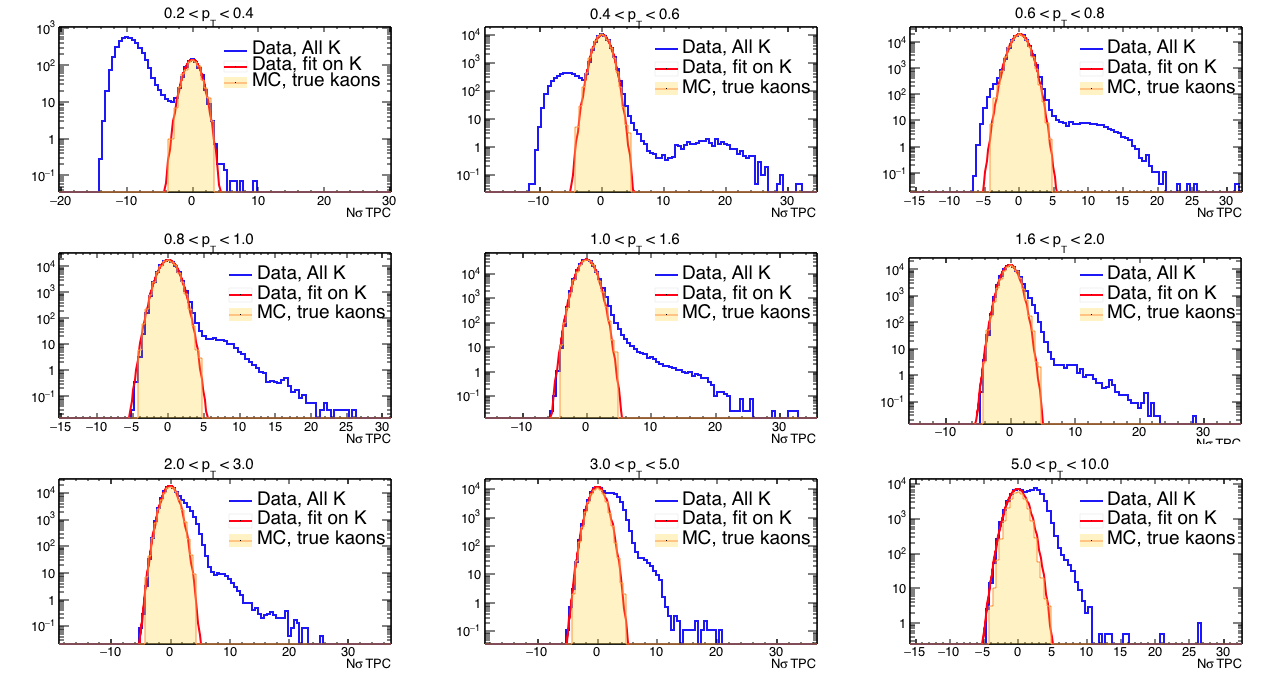
\includegraphics[angle=0, width=15cm]{./FigCap5/KaonTPCFromTOF_DataMC.png}
 \caption{N$\sigma$ distribution of d$E$/d$x$ signal in TPC for kaons selected based on TOF information in data. The distribution of true kaons form the Monte Carlo is shown in yellow. The fit to extract the kaon component from the inclusive distribution is shown in red.}
 \label{fig:DataKaonsTPC} 
\end{figure}

\begin{figure}[!h]
 \centering
 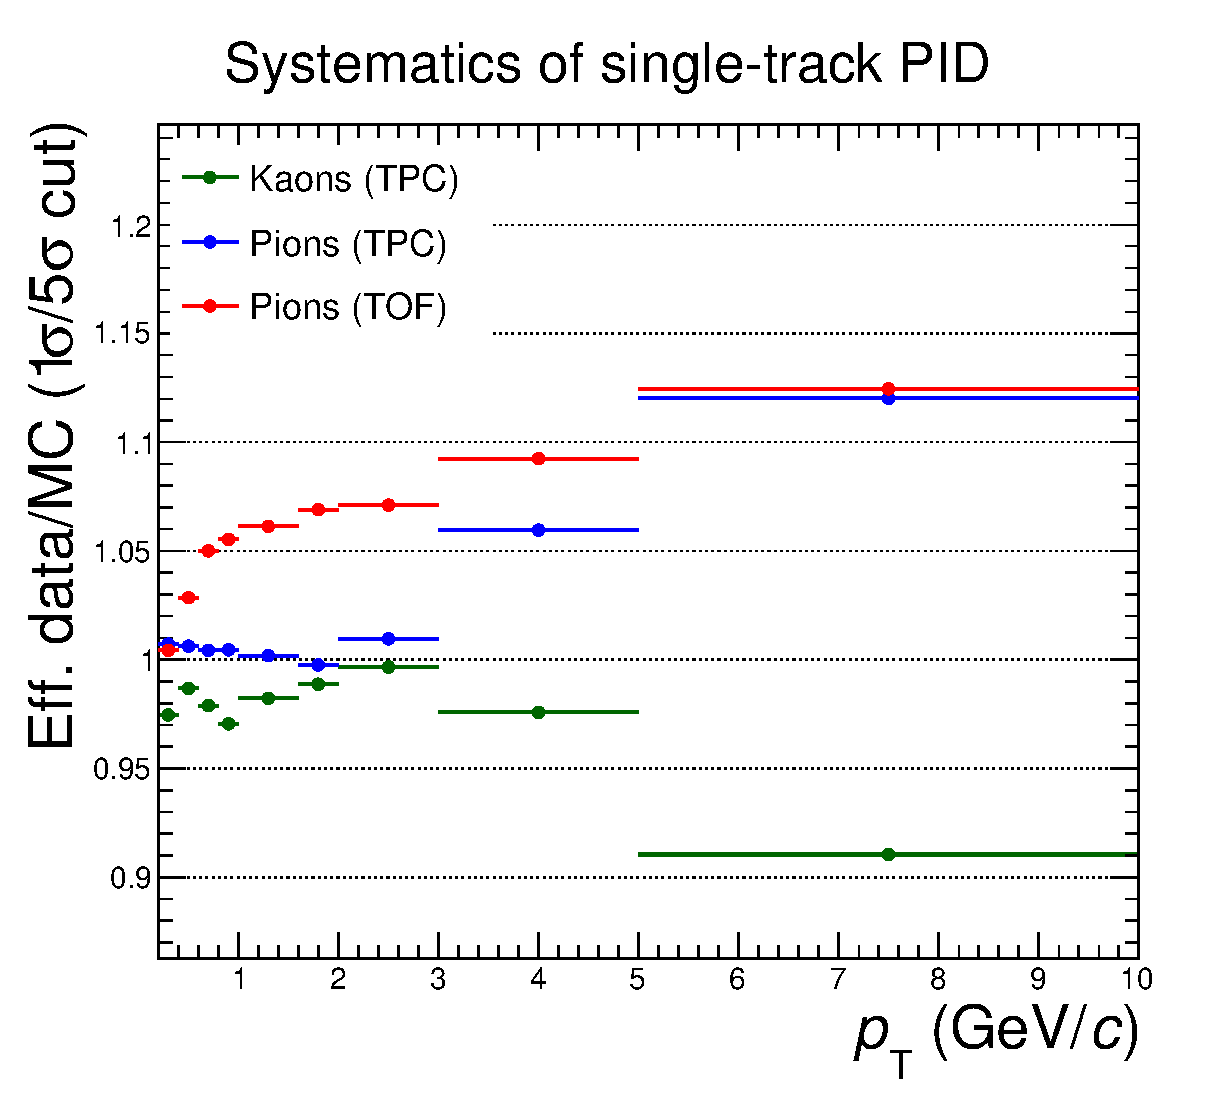
\includegraphics[angle=0, width=7cm]{./FigCap5/PIDsyst_1over5sigmaCut.eps}
 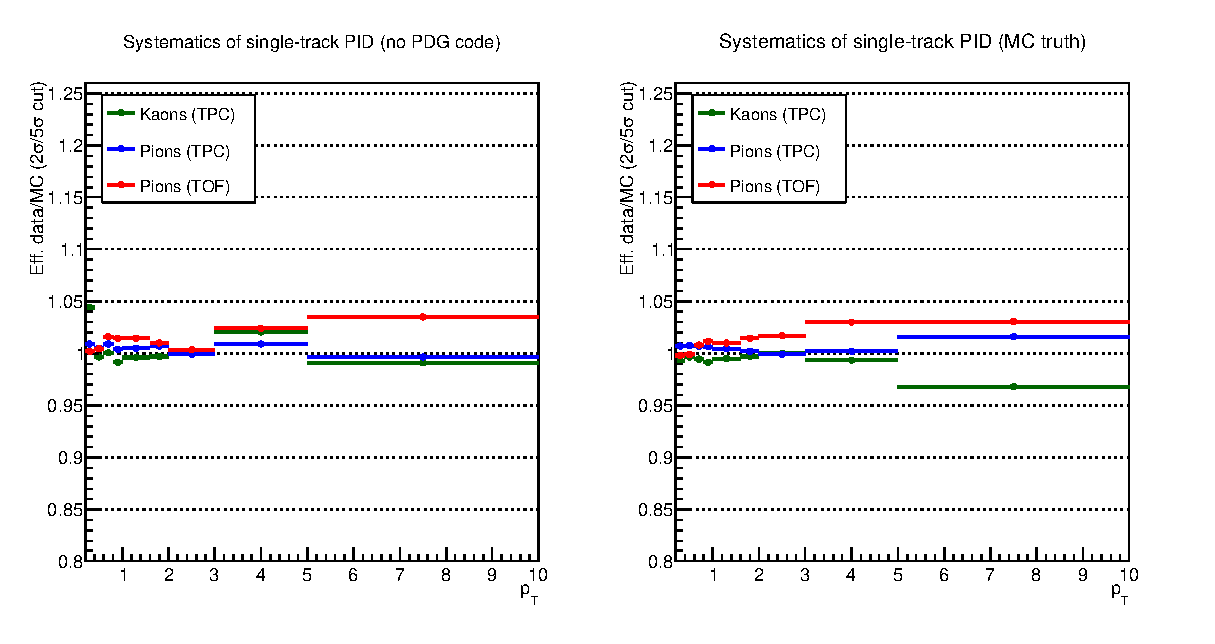
\includegraphics[angle=0, width=7cm]{./FigCap5/PIDsyst_2over5sigmaCut.eps}
 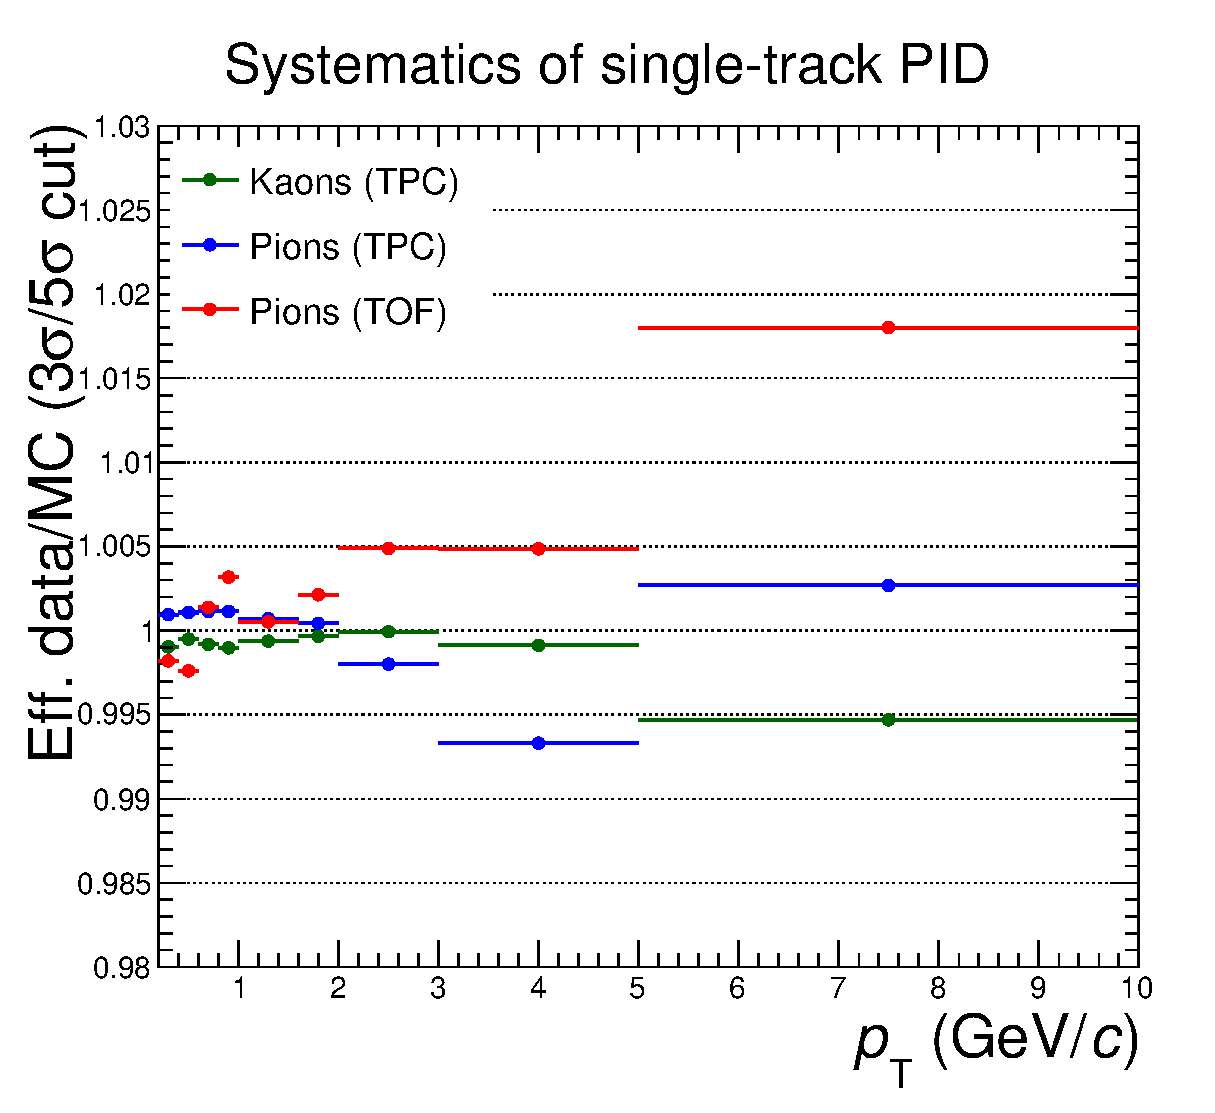
\includegraphics[angle=0, width=7cm]{./FigCap5/PIDsyst_3over5sigmaCut.eps}
 \caption{Ratios of N$\sigma$ selection efficiencies in data and MC for kaons and pions in TPC and TOF in different colours, as a function of $\pt$, for 1$\sigma$ (top left), 2$\sigma$ (top right) and 3$\sigma$ (bottom) selection, normalised to a 5$\sigma$ cut. }
 \label{fig:PerTrackPIDsys} 
\end{figure}

\begin{figure}[!h]
 \centering
 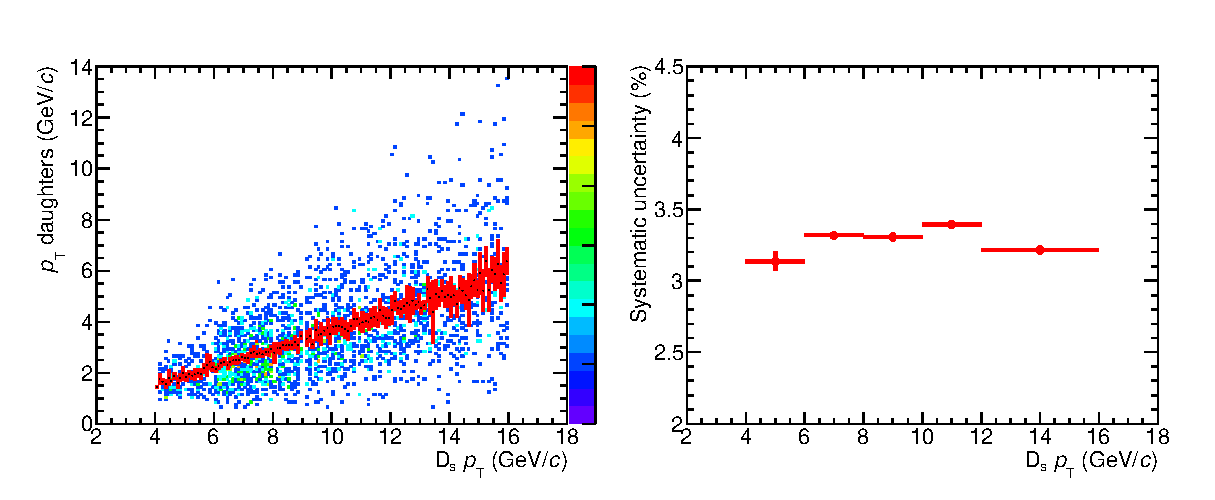
\includegraphics[angle=0, width=13cm]{./FigCap5/PIDsystDs_MCall.eps}
 \caption{Left: scatter plot of $\Ds$ daughter $\pt$ as a function of $\Ds$-meson $\pt$. Right: systematic uncertainty on the tighter PID selection used for $\Ds$ meson as a function of $\Ds$ $\pt$.}
 \label{fig:DsPIDsys} 
\end{figure}

\subsection{Generated $\pt$ shape}
The systematic effect on the efficiency due to a possible difference between 
the real and simulated $\Ds$-meson transverse momentum distributions
was estimated by using alternative $\Ds$-meson $\pt$ distributions.
In particular, the $\pt$ distributions from FONLL calculations with
and without hot-medium effects parametrised based on the $\RAA$ in central collisions from the 
TAMU~\cite{He:2014cla} model and in semi-central collisions from 
BAMPS~\cite{Uphoff:2014hza} model were used in this study.
The values assigned as systematic uncertainty are reported in 
Table~\ref{tab:sysunc_yieldtable} for the three centrality classes.


\iffalse
\begin{figure}[!htp]
\begin{center}
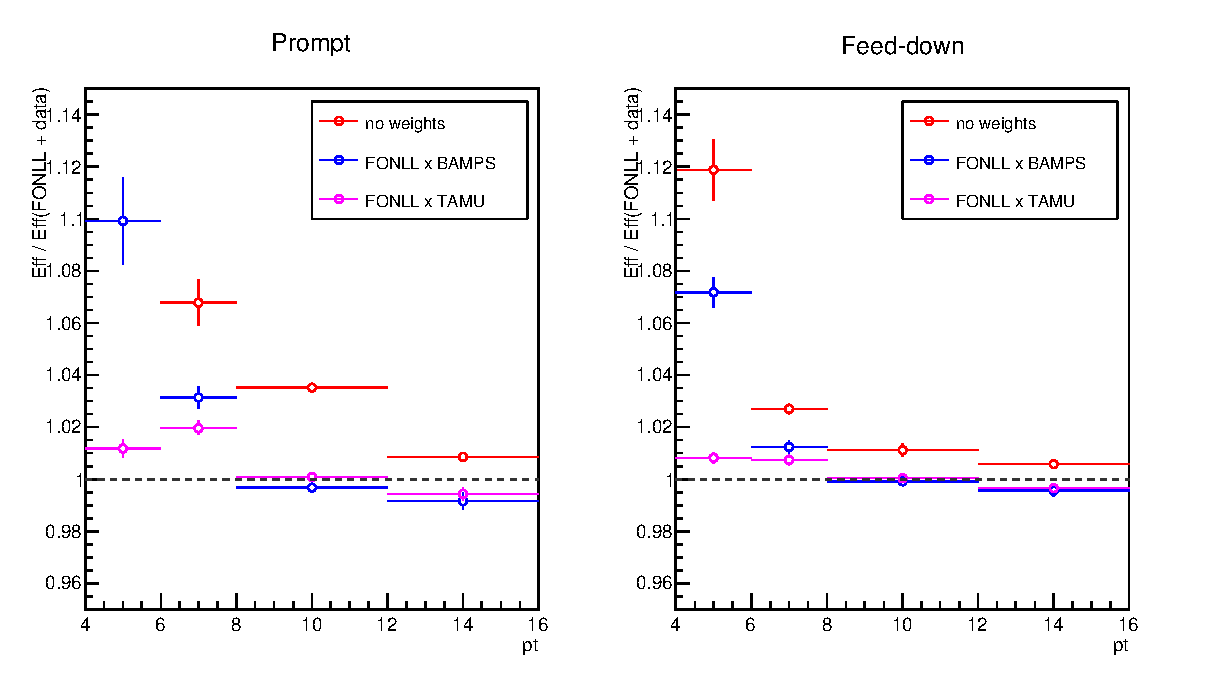
\includegraphics[angle=0, width=11.cm]{./FigCap5/MCptweights010_overFONLLdata_617.eps}   
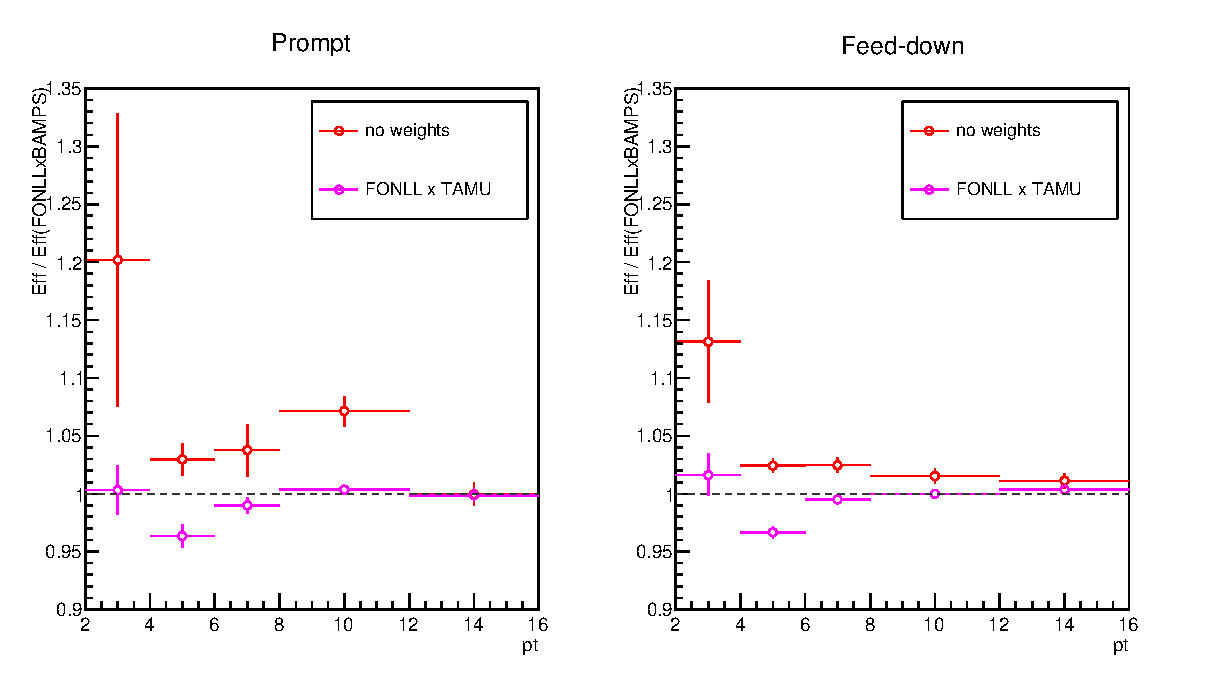
\includegraphics[angle=0, width=11.cm]{./FigCap5/MCptweights6080_overFONLLBAMPS_618.eps}   
\end{center}
\caption{Top: relative change of $\rm \Ds$ prompt and feed-down efficiencies in the 0--10\% centrality class by using FONLL  x BAMPS (blue), no (red) $\pt$-weights, or FONLL x TAMU (magenta) with respect to case of $\Dzero$ data-driven weights (default). Bottom: relative change of $\rm \Ds$ prompt and feed-down efficiencies in the 60--80\% centrality class by using no (red) $\pt$-weights, or FONLL x TAMU (magenta) with respect to case of FONLL x BAMPS weights (default).}
\label{DsMCshape_010_6080} 
\end{figure}
\fi

\subsection{Feed-down subtraction}
\label{sec:FDsystAA}
The systematic uncertainty on the correction for the contribution of feed-down from 
B-meson decays was estimated by varying i)
the $\pt$-differential B-meson cross section in the 
FONLL calculation within the theoretical uncertainties (that originate from variations of 
$b$-quark mass, perturbative scales and from uncertainties on the parton distribution functions~\cite{Cacciari:2012ny}), 
ii) the variation of the hypothesis on $\RAA^{\rm  feed-down}/\RAA^{\rm prompt} $. 
Several theoretical models predict that charm quarks lose more energy 
in the medium than heavier quarks. As a consequence, the nuclear modification 
factor of B mesons should be larger than that of D mesons and hence the ratio 
R$^{feed-down}_{AA}$/R$^{prompt}_{AA}$ should be larger than unity. 
This assumption was confirmed by the comparison of the $\RAA$ of prompt D mesons at 
$\sNN = 2.76$ TeV~\cite{Adam:2015nna} with that of J/$\psi$ from B-meson decays~\cite{Khachatryan:2016ypw} 
measured by the CMS experiment (see Sec.~\ref{sec:resAAcap2}).
If recombination plays a role in the charm hadronisation, however,  
the ratio R$^{feed-down}_{AA}$/R$^{prompt}_{AA} $ could assume values 
less than unity. The ratio of the nuclear modification factors of feed-down and 
prompt $\Ds$ mesons was therefore varied in the range 
$\frac{1}{3} < \RAA^{\rm  feed-down}/\RAA^{\rm prompt} < 3$, in 
the 0-10\% and 30-50\% centrality classes.
The relative variation of prompt $D^+_s$ yield is presented as a function of the hypothesis on  
$\RAA^{\rm  feed-down}/\RAA^{\rm prompt}$ in Fig.~\ref{fig:promptAA}
for the 0-10\% centrality class. 
respectively. The range was limited to 
$1 < \RAA^{\rm  feed-down} / \RAA^{\rm prompt} < 1.6$ 
for the centrality class 60-80\%, as anticipated in Sec.~\ref{sec:CorrectionsAA},
due to the milder medium effects.
\begin{figure}[!h]
 \begin{center}
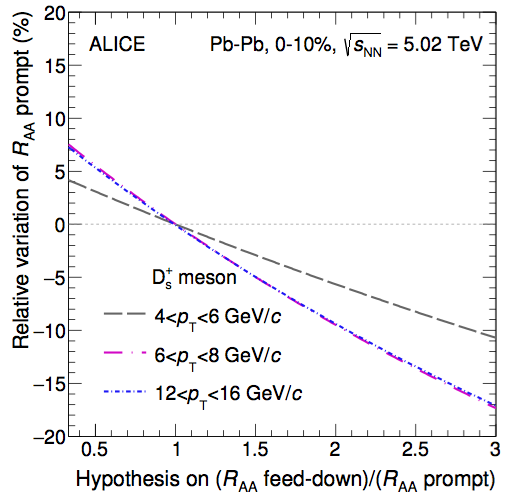
\includegraphics[width=.49\textwidth]{./FigCap5/RaaVariationVsRbHypo.png}
\end{center}
 \caption{Relative variation of of prompt $D^+_s$ yield in the 0-10\% centrality class as a function of the hypothesis on $\RAA^{\textnormal{feed-down}}/\RAA^{\rm prompt}$.}
 \label{fig:promptAA}
\end{figure}


\subsection{Track reconstruction efficiency}
\label{sec:TrackEffSystPbPb}
The procedure to estimate the systematic uncertainty due to
 tracking efficiency was discussed in Sec.~\ref{sec:TrackEffSystPP}.
The per-track uncertainty quoted to account for track-quality selection efficiencies
based on a cut variation approach is 1.5\% in the 10\% most central events and 1\% in 30-50\% and 60-80\% 
centrality classes. The systematic uncertainty on the ITS-TPC 
track-matching efficiency was estimated by comparing its values in data and simulations
after correcting for the different contribution of secondary particles, according to
the procedure described in Sec.~\ref{sec:TrackEffSystPP}.
Some discrepancies are observed in the systematic uncertainties (up to 4\%, for $2 < \pt < 4\, \Gevc$)
if the request of a point in SPD is applied or not on the tracks used to fill the DCA$_{\rm xy}$ distribution.
The two approaches have different pros and cons. The extraction of the primary
and secondary fractions from the fit to DCA$_{\rm xy}$ distribution of
tracks with a point in SPD is more robust thanks to the better resolution on the track 
parameters as compared to the TPC-only tracks. However, the request of
ITS points requires to introduce a correction factor to rescale the fraction of primary tracks in the ITS
to that in TPC. This factor is extracted from MC and it
relies on the fact that the simulation should reproduce well the data for what concerns
the dependence of the relative abundance of primary tracks on the radial distance from the beam axis.
For the case without the request of hit in the SPD, the DCA$_{\rm xy}$
resolution is worse and tracks with different impact parameter resolution are mixed. 
However, the fits can be performed with acceptable quality.
The observed discrepancy in the results between the two approaches 
may be due to the less precise estimate
of the fraction of primary tracks in the case of not requiring the SPD point, as well as
to a non valid assumption on the MC-based correction factor, in case in which 
the SPD point is required. For this reason, the systematic 
uncertainty on the ITS-TPC matching efficiency for the single track was
assigned by averaging the two results, and the resulting plot is shown in Fig.~\ref{fig:systME_AA}.\\
\begin{figure}
\centering
 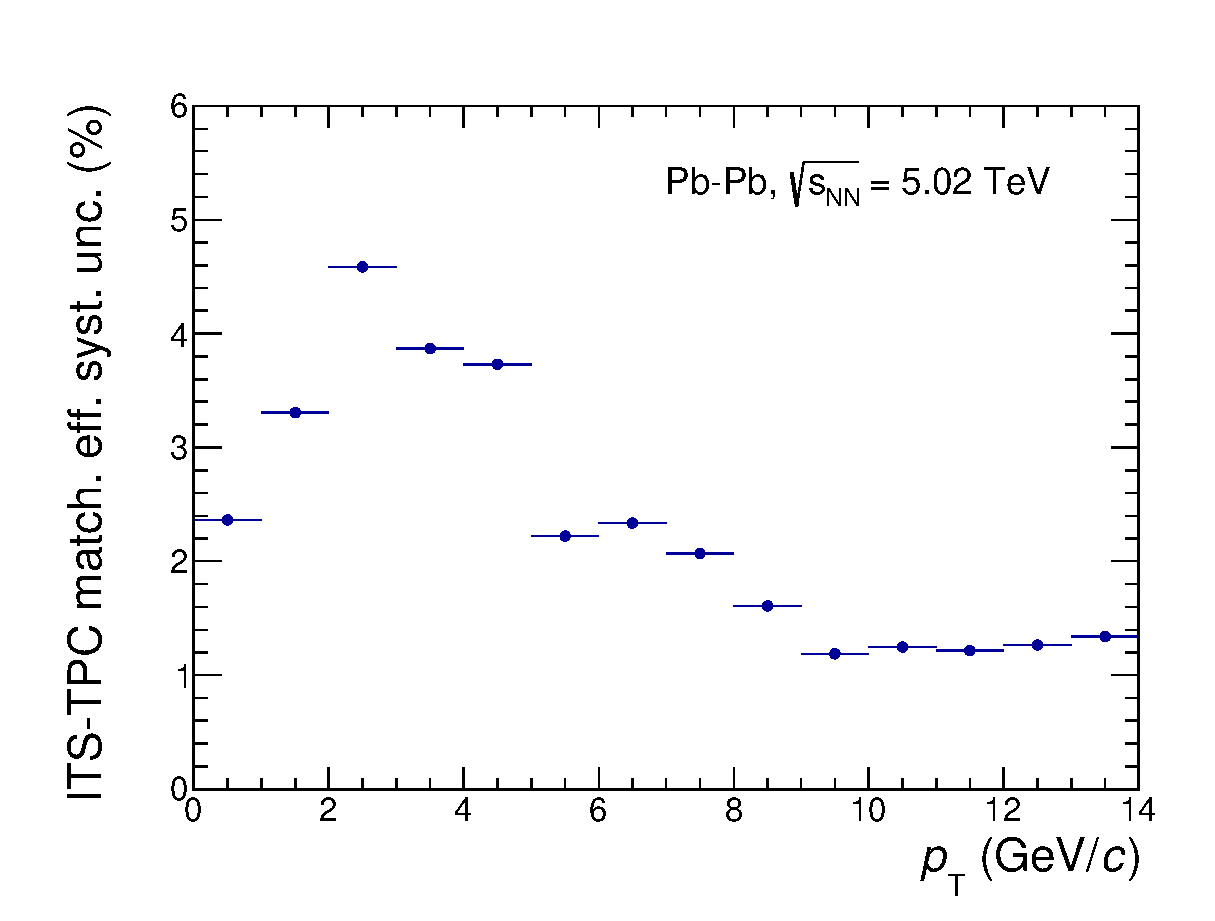
\includegraphics[width=0.6\textwidth]{FigCap5/MatchEffSyst_LHC15o_16g1abc_wcutV0multTPCout_wTOFbc_AverITSTPCtracks.eps}
 \caption{Systematic uncertainty on ITS-TPC track-matching efficiency in Pb-Pb at $\sNN=5.02$ TeV as a function of $\pt$ of the track.}
 \label{fig:systME_AA}
\end{figure}


The values of the systematic uncertainties on the $\Ds$-meson corrected yields
are summarised in Tab.~\ref{tab:sysunc_yieldtable}, in the $\pt$ intervals considered in 
the analysis. The uncertainties on the fraction of the hadronic cross section used in the Glauber fit to determine
the centrality are shown as well in the Table.
\begin{table}[!h]
\centering
\begin{tabular}{|l|l|l|c|c|c|c|c|c|}
\hline
\multicolumn{6}{|c|}{0--10\% centrality class}       \\                                                                                                                                                                                                                                               \hline
$\pt$ interval ($\gev/c$) & 2--4        &    4--6          & 6--8      &   8--12            & 12--16                  \\ 
\hline
Yield extraction & - & 6\% & 6\%& 6\%& 6\%\\
Tracking efficiency & -  & 11\% &11.5\% &11.5\% & 10\% \\
PID efficiency & -  & 3\%& 3\% & 0\%&  0\%\\
Cut efficiency & -  & 10\%& 10\%& 10\%& 10\%\\
MC $\pt$ shape & -  & 7\%& 2\%& 1\%& 0\% \\
Feed-down (FONLL scales) & -  & $^{+2.2\%}_{-2.9\%}$ &$ ^{+3.5\%}_{-4.6\%} $& $^{+3.1\%}_{-3.9\%}$& $^{+3.1\%}_{-3.7\%}$\\
Feed-down ($\RAA^{\rm feed-down}$ hypothesis)  & - & $^{+4.0\%}_{-10.3\%}$& $^{+6.6\%}_{-15.7\%} $&$ ^{+6.3\%}_{-14.7\%}$ & $^{+6.7\%}_{-15.6\%} $\\
\hline
Centrality limit & \multicolumn{5}{c|}{0.1\%}  \\
\hline
\hline
Branching ratio & \multicolumn{5}{c|}{3.5\%}  \\
\hline
\hline
Total  & - & $^{+20.7\%}_{-22.8\%}$& $^{+18.6\%}_{-23.6\%}$ & $^{+17.9\%}_{-22.5\%}$ & $^{+17.1\%}_{-22.3\%}$  \\
\hline
\hline
\multicolumn{6}{|c|}{30--50\% centrality class}       \\                                                                                                                                                                                                                                               \hline
$\pt$ interval ($\gev/c$)   & 2--4     &    4--6          & 6--8      &   8--12            & 12--16                  \\ 
\hline
Yield extraction & -  & 9\% & 7\%& 6\%& 5\%\\
Tracking efficiency & -  & 11\% &11.5\% &11.5\% & 10\% \\
PID efficiency  & - & 3\%& 3\% & 0\%&  0\%\\
Cut efficiency  & - & 15\%& 15\%& 10\%& 10\%\\
MC $\pt$ shape & -  & 4\%& 1\%& 2\%& 1\% \\
Feed-down (FONLL scales) & -  &$ ^{+3.3\%}_{-4.2\%}$ & $^{+4.5\%}_{-5.8\%} $&$ ^{+3.5\%}_{-4.5\%}$& $^{+2.5\%}_{-3.0\%}$\\
Feed-down ($\RAA^{\rm feed-down}$ hypothesis)  & - & $^{+5.5\%}_{-13.4\%}$& $^{+7.8\%}_{-18.1\%} $&$ ^{+7.2\%}_{-16.8\%} $& $^{+5.6\%}_{-13.8\%}$ \\
\hline
Centrality limit & \multicolumn{5}{c|}{0.1\%}  \\
\hline
\hline
Branching ratio & \multicolumn{5}{c|}{3.5\%}  \\
\hline
\hline
Total  & - & $^{+20.7\%}_{-24.8\%}$& $^{+24.5\%}_{-29.6\%}$ & $^{+16.3\%}_{-22.4\%}$ & $^{+14.7\%}_{-19.5\%}$  \\
\hline
\hline
\multicolumn{6}{|c|}{60--80\% centrality class}       \\                                                                                                                                                                                                                                               \hline
$\pt$ interval ($\gev/c$)  &2--4      &    4--6          & 6--8      &   8--12            & 12--16                  \\ 
\hline
Yield extraction & 10\%  & 6\% & 6\%& 5\%& 5\%\\
Tracking efficiency & 11\%  & 11\% &11.5\% &11.5\% & 10\% \\
PID efficiency  & 3\% & 3\%& 3\% & 3\%&  3\%\\
Cut efficiency  & 14\% & 10\%& 12\%& 10\%& 12\%\\
MC $\pt$ shape  & 6\% & 2\%& 2\%& 1\%& 1\% \\
Feed-down (FONLL scales) & $^{+7.2\%}_{-8.5\%} $& $^{+4.5\%}_{-6.0\%}$ & $^{+6.2\%}_{-8.0\%}$ & $^{+5.2\%}_{-6.6\%}$& $^{+2.9\%}_{-3.4\%}$\\
Feed-down ($\RAA^{\rm feed-down}$ hypothesis)  & $^{+3.4\%}_{-3.1\%} $& $^{+2.6\%}_{-2.6\%}$& $^{+3.6\%}_{-3.4\%}$ &$ ^{+3.3\%}_{-3.1\%} $& $^{+2.0\%}_{-1.9\%}$ \\
\hline
Centrality limit & \multicolumn{5}{c|}{0.1\%}  \\
\hline
\hline
Branching ratio & \multicolumn{5}{c|}{3.5\%}  \\
\hline
\hline
Total  & $^{+28.4\%}_{-28.7\%}$& $^{+18.3\%}_{-18.7\%}$ & $^{+21.4\%}_{-22.0\%}$ & $^{+18.0\%}_{-18.4\%}$  & $^{+17.7\%}_{-17.7\%}$  \\
\hline
\end{tabular}
\caption{Relative systematic uncertainties on the $\pt$-differential yields of $\Ds$ in the 0-10\%, 30-50\% and 60-80\% centrality classes.}
\label{tab:sysunc_yieldtable}
\end{table}

\section{Nuclear modification factor in Pb-Pb collisions}
\label{sec:RAA}
The nuclear modification factor $\RAA$ of prompt $\Dsplus$ mesons was defined as follows:
\begin{equation}
\label{eq:RAADs}
\RAA (\pt) = \frac{1}{\langle \TAA \rangle} \frac{{\rm d} N_{\rm AA}/{\rm d}\pt}{{\rm d} \sigma_{\rm pp}/{\rm d} \pt},
\end{equation}
where ${\rm d} N_{\rm AA}/{\rm d}\pt$ is the $\pt$-differential yield of prompt $\Dsplus$ mesons
of Eq.~\ref{eq:dNdpt}, $\langle \TAA \rangle$ is the 
average nuclear overlap function for the considered centrality class and ${\rm d} \sigma_{\rm pp}/{\rm d} \pt$ is 
the $\Dsplus$ $\pt$-differential cross section in pp collisions at $\s = 5.02$ TeV.
\section{Systematic uncertainty on the $\RAA$}
\label{sec:SystRAA}
The systematic uncertainty on the $\Raa$ measurement was computed by combining the uncertainties  
on the $\Ds$-meson yield in Pb-Pb collisions described in Sec.~\ref{sec:systematics} and those 
on the pp reference cross-section. The systematic 
uncertainty on the feed-down subtraction deriving from
the variation of the parameters of the FONLL calculation was considered to be
correlated between the $\PbPb$ and pp measurements. All the 
other sources of systematic uncertainties were treated as uncorrelated. 
An additional source of systematic uncertainty originates from the uncertainty
on the $\langle T_{\rm AA}$ used in the $\Raa$ calculation.

\subsection{Proton-proton reference}
\label{sec:PPrefSyst}
The $\pt$-differential cross section of prompt $\Dsplus$ mesons with 
$|y|<0.5$ in pp collisions at $\sqrt s=5.02~\tev$, used as reference 
for the nuclear modification factor, was obtained by scaling the 
measurement at $\sqrt{s}=7~\TeV$ described in 
Chapter~\ref{chap:pp}~\cite{Acharya:2017jgo} to $\s = 5.02$ TeV 
with FONLL calculations~\cite{Cacciari:2012ny}. 
This measurement 
reaches up to $12~\Gevc$ for $\Ds$ mesons.
In particular, the value of the cross section measured at $\s$ = 7 TeV 
at central rapidity $|y| < 0.5$ was scaled in each $\pt$ interval by 
the ratio of the FONLL predictions at the two energies in the same rapidity region as follows:
\begin{equation}
\label{eq:scalingPP}
\sigma^{\rm 5.02 TeV}_{\rm scaled} (\pt) = \frac{\sigma^{\rm 5.02 TeV}_{\rm FONLL} (\pt)}{\sigma^{\rm 7 TeV}_{\rm FONLL} (\pt)} \sigma^{\rm 7 TeV}_{\rm meas} (\pt).
\end{equation}
The uncertainty on the pp reference 
has two contributions. The first one is the uncertainty on the measured 
$\pt$-differential $\Dsplus$-meson cross section at $\sqrt s=7$~TeV.
The second contribution is the $\pt$-dependent scaling factor 
from $\sqrts=7~\tev$ to $\sqrts=5.02~\tev$, determined by varying
the FONLL parameters (charm-quark mass, factorisation and renormalisation scales) 
as described in Sec.~\ref{sec:BfdSub} and in~\cite{Averbeck:2011ga}. The values of these parameters were 
varied coherently at the two energies. The scaling factor 
and its uncertainties from FONLL calculations are shown in Fig.~\ref{fig:FONLLscalFact}.
In the interval $12<\pt<16~\Gevc$, the FONLL calculation at 
$\sqrt s=5.02~\tev$~\cite{Cacciari:2012ny} was used as a reference 
by scaling the values to match the central value of the data at lower $\pt$. 
\begin{figure}[!h]
\centering
 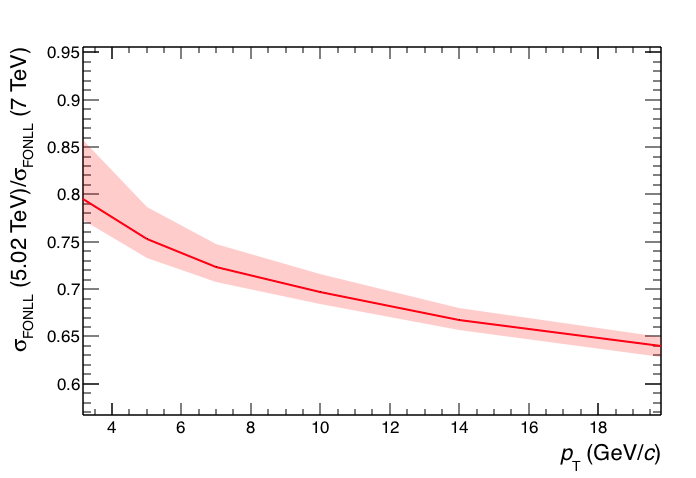
\includegraphics[width=0.6\textwidth]{FigCap5/FONLLscaling7To5TeV.png}
 \caption{Scaling factor obtained for cross sections of prompt $\Dsplus$ mesons in pp collisions, from $\sqrts=7~\tev$ to $\sqrts=5.02~\tev$, as a function of $\pt$. The red line corresponds to the result used as central value for the correction; the uncertainty bands are obtained from variation of FONLL perturbative parameters. }
 \label{fig:FONLLscalFact}
\end{figure}


\iffalse
The cross section measurements of $\Ds$ meson in pp collisions at $\s = $ 7 TeV 
is limited to $\pt < 12 \, \Gevc$. For the interval $12 \leq \pt < 16 \, \Gevc$ 
the pp reference was obtained using the cross section from the FONLL calculation at $\s = 5.02$ TeV. 
Since the central value of the FONLL calculation at $\s = 5.02$ TeV underestimates the measurement 
for $\pt > 5 \, \Gevc$ at both ?and ?s = 7 TeV [45, 60], the FONLL cross section was multiplied by a scaling factor (?) 

The factor ? was determined by fitting with a constant the data-to-theory ratio at ?s = 7 TeV in the
?s = 2.76 TeV are less precise, they do not interval 5 < pT < 16 GeV/c. Since the measurements at ?
?constrain further the scaling factor. 
\fi
This procedure is described in Ref.~\cite{Adam:2015sza}. The total 
systematic uncertainty on the $\pt$-extrapolated cross section is about 
$^{+29}_{-42}\%$ for $\Ds$ in the $\pt$ interval 12--16~$\Gevc$.


\subsection{Normalization}
\label{sec:NormalizSyst}
The uncertainties on the $\RAA$ normalisation are the quadratic sum of 
(i) the normalisation uncertainty on the integrated luminosity used for the measurement of the $\Ds$ cross section in pp collisions (3.5\%), 
(ii) the uncertainty on $\langle T_{\rm AA} \rangle$, which ranges from 3.3\% to 6.2\% depending on the centrality, and
(iii) the uncertainty on the fraction of the hadronic cross section used in the 
Glauber fit to determine the centrality ($<0.1\%$, $2\%$ and $3\%$ for the 0--10\%, 30--50\% 
and 60--80\% centrality classes, respectively)~\cite{Adam:2015sza}, while the branching ratio uncertainty cancels out in the 
ratio.

\begin{table}[!h]
\centering
\begin{tabular}{|l|l|l|c|c|c|c|c|}
\hline
\multicolumn{6}{|c|}{0--10\% centrality class}       \\                                                                                                                                                                                                                                               \hline
$\pt$ interval ($\gev/c$)     & 2--4    &    4--6          & 6--8      &   8--12            & 12--16                  \\ 
\hline
Data syst. AA    &   -     & 20.1\%  & 17.0\%  & 16.5\%  & 15.5\% \\
Data syst. pp + $\s$-scaling  &   -      & $^{+13.2\%}_{-13.7\%}$  & $^{+12.9\%}_{-13.2\%}$  & $^{+12.9\%}_{-13.0\%}$  & $^{+29.3\%}_{-42.3\%}$\\
Feed-down (FONLL scales)  &   -    & $^{+1.2\%}_{-0.9\%}$  & $^{+0.2\%}_{-0.1\%}$  & $^{+0.7\%}_{-0.4\%}$  & $^{+3.1\%}_{-3.7\%}$ \\
Feed-down ($\RAA^{\rm feed-down}$ hypothesis)   &   -        & $^{+3.9\%}_{-10.2\%}$  & $^{+6.6\%}_{-15.6\%}$  & $^{+6.1\%}_{-14.7\%}$  & $^{+6.5\%}_{-15.6\%}$\\
\hline
Normalisation     & \multicolumn{5}{|c|}{4.8\%} \\
\hline
\hline
Total  &   - & $^{+24.4\%}_{-26.5\%}$  & $^{+22.4\%}_{-26.6\%}$  & $^{+21.8\%}_{-25.7\%}$  & $^{+34.0\%}_{-47.8\%}$\\
\hline
\hline
\multicolumn{6}{|c|}{30--50\% centrality class}       \\                                                                                                                                                                                                                                               \hline
$\pt$ interval ($\gev/c$) & 2--4        &    4--6          & 6--8      &   8--12            & 12--16                  \\ 
\hline
Data syst. AA       &   -     & 24.0\%  & 22.7\%  & 14.2\%  & 13.4\%\\
Data syst. pp + $\s$-scaling  &   -  & $^{+13.2\%}_{-13.7\%}$  & $^{+12.9\%}_{-13.2\%}$  & $^{+12.9\%}_{-13.0\%}$  & $^{+29.3\%}_{-42.3\%}$ \\
Feed-down (FONLL scales)   &   -   & $^{+0.1\%}_{-0.1\%}$  & $^{+1.0\%}_{-1.0\%}$  & $^{+0.1\%}_{-0.1\%}$  & $^{+2.5\%}_{-3.0\%}$   \\
Feed-down ($\RAA^{\rm feed-down}$ hypothesis)  &   -       & $^{+5.5\%}_{-13.3\%}$  & $^{+7.8\%}_{-18.0\%}$  & $^{+7.1\%}_{-16.7\%}$  & $^{+5.6\%}_{-13.8\%}$\\
\hline
Normalisation     & \multicolumn{5}{|c|}{4.9\%} \\
\hline
\hline
Total  &   - & $^{+28.0\%}_{-30.7\%}$  & $^{+27.3\%}_{-31.9\%}$  & $^{+20.4\%}_{-25.5\%}$  & $^{+32.8\%}_{-46.6\%}$ \\
\hline
\hline
\multicolumn{6}{|c|}{60--80\% centrality class}       \\                                                                                                                                                                                                                                               \hline
$\pt$ interval ($\gev/c$)  & 2--4       &    4--6          & 6--8      &   8--12            & 12--16                  \\ 
\hline
Data syst. AA        &   27.2\%    & 17.6\%& 20.2\%& 16.9\%& 17.3\%\\
Data syst. pp + $\s$-scaling  &    $^{+12.9\%}_{-14.5\%}$    & $^{+13.2\%}_{-13.7\%}$  &$^{+12.9\%}_{-13.2\%}$ &$^{+12.9\%}_{-13.0\%} $ &$^{+29.3\%}_{-42.3\%}$  \\
Feed-down (FONLL scales)   &    $^{+3.3\%}_{-4.2\%}$   &  $^{+1.4\%}_{-2.0\%}$& $^{+2.5\%}_{-3.4\%}$&  $^{+1.6\%}_{-2.1\%}$&  $^{+2.9\%}_{-3.4\%}$\\
Feed-down ($\RAA^{\rm feed-down}$ hypothesis)   &   $^{+3.4\%}_{-3.1\%}$     & $^{+2.6\%}_{-2.5\%}$& $^{+3.6\%}_{-3.3\%}$& $^{+3.3\%}_{-3.1\%}$& $^{+2.0\%}_{-1.9\%}$\\
\hline
Normalisation     & \multicolumn{5}{|c|}{6.7\%} \\
\hline
\hline
Total  &   $^{+30.5\%}_{-31.1\%}$ & $^{+22.2\%}_{-22.5\%}$& $^{+24.4\%}_{-24.6\%}$& $^{+21.6\%}_{-21.7\%}$&$^{+34.2\%}_{-45.9\%}$\\
\hline
\hline
\end{tabular}
\caption{Relative systematic uncertainties on the $\RAA$ of $\Ds$ in the 0-10\%, 30-50\% and 60-80\% centrality classes.}
\label{tab:sysunc_yieldtable}
\end{table}

\section{$\Ds$ elliptic flow}
In this section, the first measurement of the $v_2$ of prompt
$\Ds$ mesons in Pb-Pb collisions at 
$\sqrtsNN = 5.02$~$\TeV$ is reported. The analysis was carried 
out for the 30-50\% centrality class, because it is the centrality
interval where the elliptic flow reaches its maximum value~\cite{Adam:2016izf}. 

\subsection{Event characterization: event plane}
\label{sec:EventPlane}
The measurement of the azimuthal anisotropy of charm and beauty hadrons
with respect to the symmetry plane of the collision can provide important information on the properties of the QGP medium 
and the interactions between heavy quarks and the medium.
The $\pt$-differential azimuthal distribution of produced particles can be described by a Fourier series:
\begin{equation}
\label{eq:fourier}
\frac{{\rm d}^2N}{{\rm d} \varphi {\rm d}\pt} =  \frac{{\rm d}N}{2\pi {\rm d}\pt} \Big [ 1+ 2 \sum_{n=1}^{\infty} v_n(\pt) \,{\rm cos} \,n(\varphi- \Psi_n)\Big ], 
\end{equation}
where $v_n$ are the Fourier coefficients, that can be evaluated as 
$v_n = \langle {\rm cos} \, n(\varphi - \Psi_n)\rangle$ and $\langle \rangle$ indicates an average over 
 all particles in all events, with their azimuthal angle $\varphi$ in a given rapidity and $\pt$ 
 momentum at a fixed centrality. In Eq.~\ref{eq:fourier},
$\Psi_n$ is the initial-state spatial plane of symmetry (reaction plane) of
 the $n^{\rm th}$ harmonic defined by the geometrical distribution of the nucleons participating in the collision.
The symmetry plane $\Psi_n$ of a given $n^{\rm th}$ harmonic is estimated 
 event-by-event from the azimuthal distribution of the produced particles
via the $n^{th}$-harmonic event-plane angle, $\psi_n^{\rm EP}$.
For a given harmonic $n$, one constructs the two-dimensional event-plane 
vector $\vec{Q}_n$:
\begin{equation}
\label{eq:qvector}
 \vec{Q}_n= {Q_{n,x} \choose Q_{n,y}} = {\sum_{i=0}^{N} w_i \cos (n\varphi_i) \choose \sum_{i=0}^{N} w_i \sin (n\varphi_i)}.
\end{equation}
The sums run over all reconstructed tracks in the case 
of the TPC, or over the scintillator tiles of the V0 detector.
The angle $\varphi_i$ is the azimuthal emission angle of the centre of the $i^{th}$ particle or the 
azimuthal coordinate of the $i^{th}$ detector element, respectively. 
For TPC tracks the weight $w_i$ can be unity or a specific 
function of $\pt$, useful to enhance the 
contribution of particle with large flow, improving 
the resolution on the event plane. For segmented detectors, $w_i$ is the amplitude of the 
signal measured in the $i^{th}$ detector element. The observed plane 
angle of the $n^{th}$ harmonic is given by the orientation of $\vec{Q}_n$:
\begin{equation}
\psi_n = \dfrac{1}{n} \tan^{-1} \left(\dfrac{Q_{n,y}}{Q_{n,x}}\right).
\end{equation}
Due to the finite number of detected particles, the
angular resolution on the reaction plane $\Psi_{\rm RP}$ is limited and 
can be estimated for the $n^{th}$ harmonic as:
\begin{equation}
R_n = \langle {\rm cos}[n({\rm \psi}_n-{\rm \Psi}_{\rm RP})]) \rangle ,
\end{equation}
where the angle brackets denote an average over a large event sample.
The resolution term must be used to correct the Fourier coefficients as:
\begin{equation}
v'_n = \frac{v_n}{R_n}.
\end{equation}
It can be demonstrated that the the event plane resolution correction factor
can be expressed as~\cite{Poskanzer:1998yz}:
\begin{equation}
\label{eq:epreso}
\left\langle \cos [km\left( \psi_m-\Psi_{\rm RP}\right)]\right\rangle = \sqrt{\dfrac{\pi }{8}} \chi_m \cdot {\rm e}^{-\chi_m^2/4} \cdot I_{(k-1)/2}(\chi_m^2/4)+I_{(k+1)/2}(\chi_m^2/4),
\end{equation}
where the equation has been written in terms of $km$ 
instead of $n$, $\chi_m= v_m/\sigma = v_m\sqrt{2N}$ ($N$ is the multiplicity) is the variable concerning the
resolution, $I_\nu$ is the Bessel function of order $\nu$ and
$k$ is an integer number that accounts for the fact that the 
event plane of $m^{th}$ order can be used to compute all Fourier harmonics that are multiples
of $m$ (i.e. $km$). The resolution correction factor from Eq.~\ref{eq:epreso} is
drawn in Fig.~\ref{fig:resoBessel} as a function of $\chi_m$, for 
different values of $k$. 
The mean cosine values are less than one, thus the 
correction always increases the Fourier coefficients.
\begin{figure}
\centering
 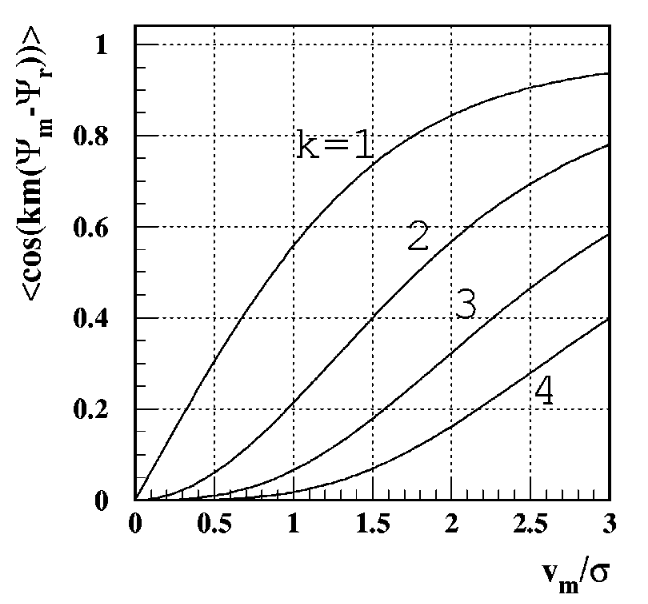
\includegraphics[width=0.5\textwidth]{FigCap5/resolBessel.png}
 \caption[Event plane resolution vs $\chi_m$]{The event plane resolution for the $n^{ th}$ ($n=km$, according the conventions of Eq.~(\ref{eq:epreso})) harmonic of the particle distribution with respect to the $m^{ th}$ harmonic plane, as a function of $\chi_m$.}
 \label{fig:resoBessel}
\end{figure}
To estimate the event plane resolution, the correlations of the event planes determined
from different samples of tracks, or different detectors are exploited.
If the full sample of tracks can be divided into two independent sub-samples 
$a$ and $b$, with same multiplicity and rapidity coverage,
the following relation holds for the correlations between the
two independent sub-sets and the true event plane:
\begin{equation}
\langle {\rm cos} [n({\rm \psi}^a_n-{\rm \psi}^b_n)) \rangle = 
\langle {\rm cos} [n({\rm \psi}^a_n-{\rm \Psi}_{\rm RP})] \rangle \langle {\rm cos} [n({\rm \psi}^b_n-{\rm \Psi}_{\rm RP})] \rangle .
\end{equation}
Since, given the conditions above, the resolution of each sub-sets is expected 
to be the same, their resolution can be obtained 
once the correlation between the two samples is known:
\begin{equation}
R_{n, sub} = \langle {\rm cos} [n({\rm \psi}^a_n-{\rm \Psi}_{\rm RP})] \rangle = \sqrt{\langle {\rm cos} [n({\rm \psi}^a_n-{\rm \psi}^b_n)] \rangle}.
\end{equation}
If the two sub-events are not equal or have different rapidity coverage,
at least three sub-samples are needed to determine the 
event-plane resolution in each of them. In this case, 
the resolution of the first sub-set $a$ is determined as:
\begin{equation}
 \langle {\rm cos} [n({\rm \psi}^a_n-{\rm \Psi}_{\rm RP})] \rangle = 
\sqrt{\frac{\langle\cos [n(\psi_n^a-\psi_n^c)] \rangle \langle\cos [n(\psi_n^a-\psi_n^b)] \rangle}{\langle\cos [n(\psi_n^b-\psi_n^c)] \rangle}}\, .
\end{equation}

\begin{figure}
\centering
  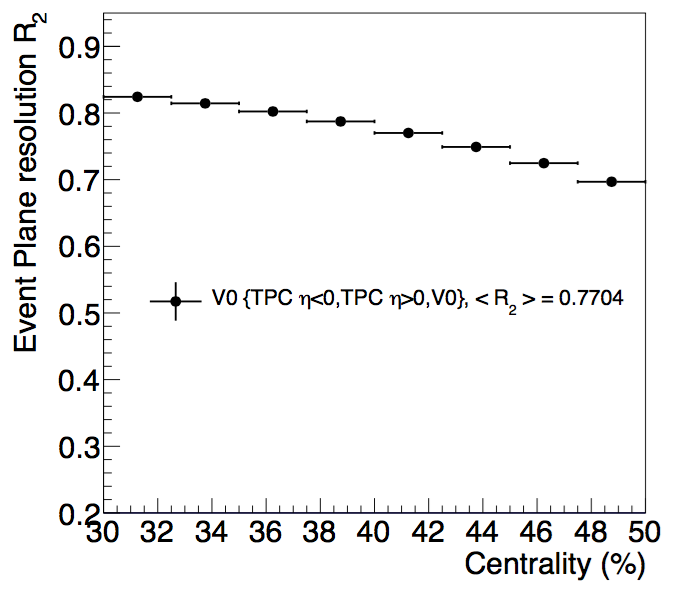
\includegraphics[width=.49\textwidth]{FigCap5/resoEP3050.png}
%  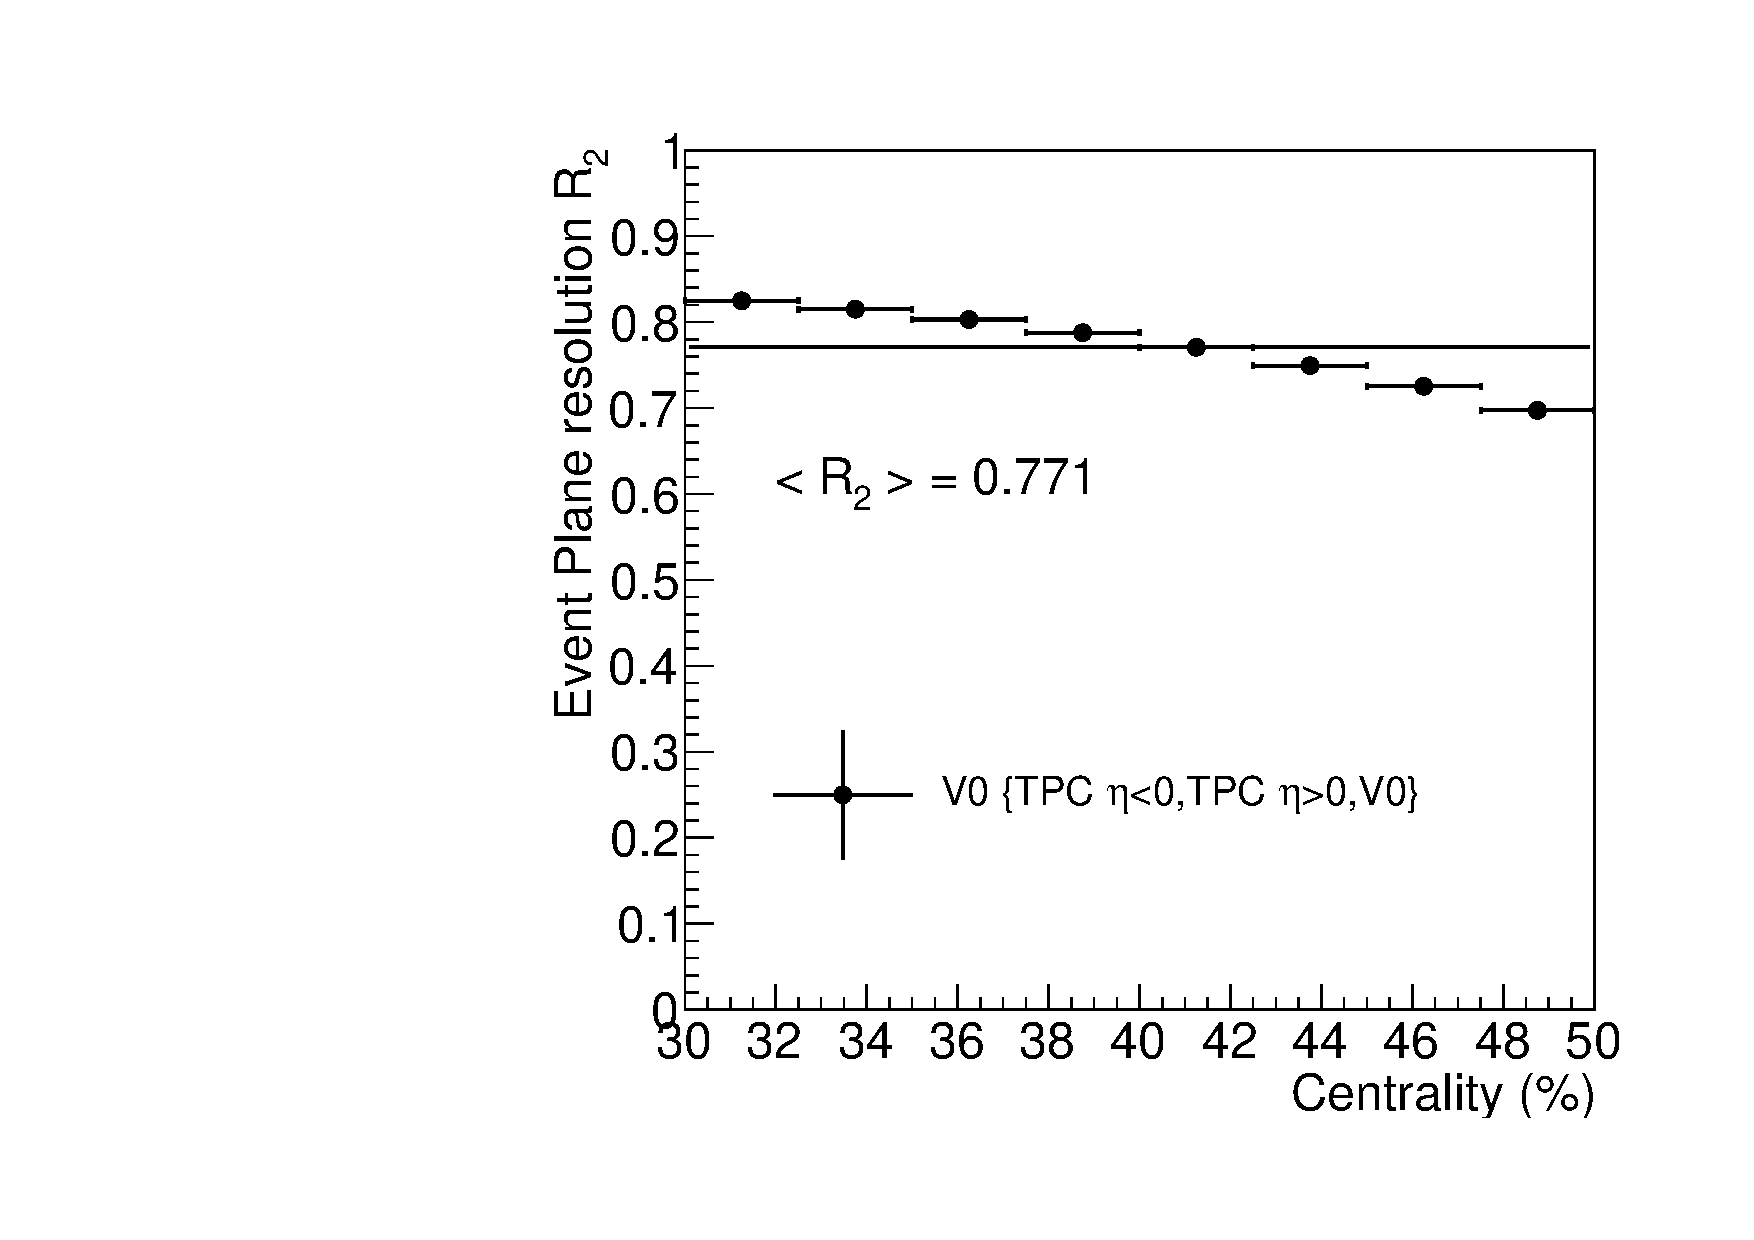
\includegraphics[width=.49\textwidth]{FigCap5/EPresolution_VZERO.pdf}
  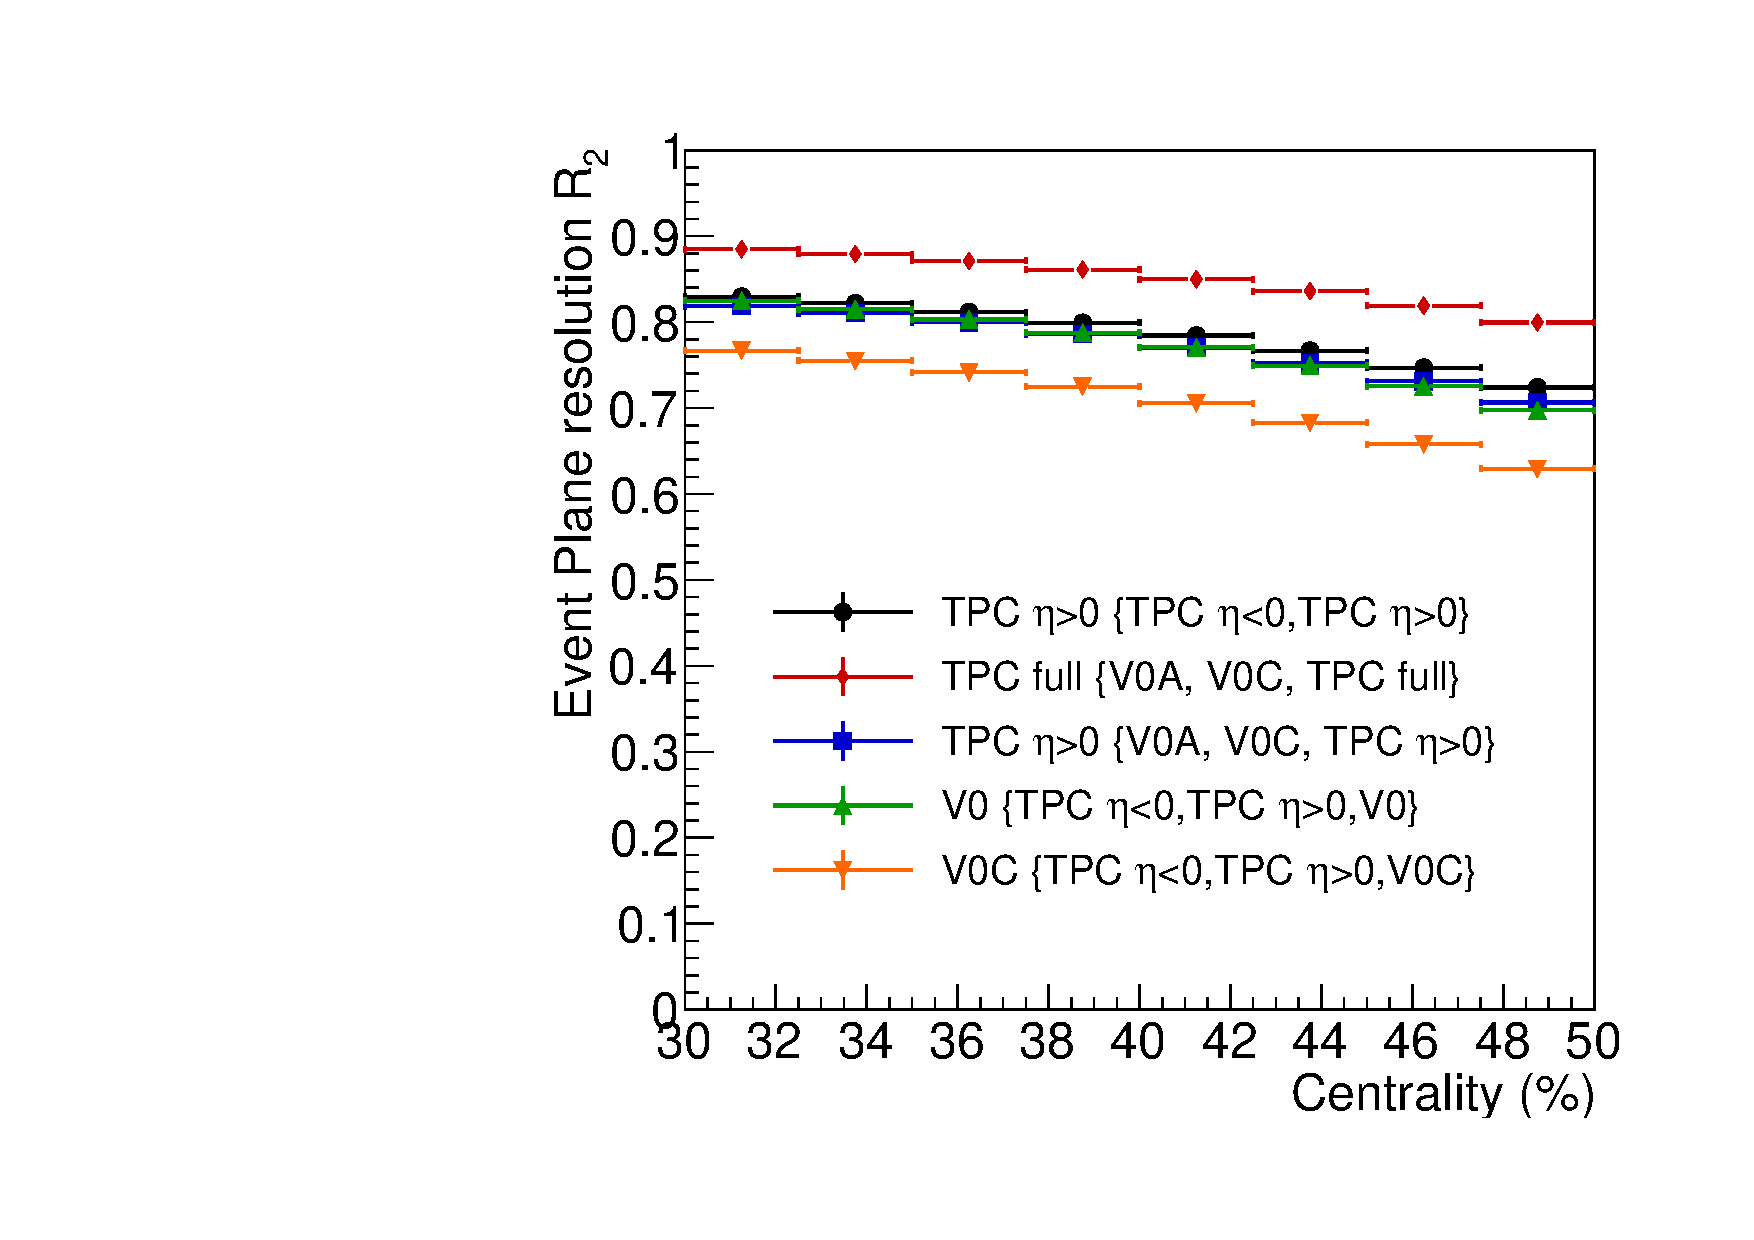
\includegraphics[width=.49\textwidth]{FigCap5/EPresolution_comparison.pdf}
\caption{$R_2$ resolution as a function of centrality estimated with default configuration (left panel) and with 5 different detector configurations (right) for the 30--50\% centrality class.}
\label{fig:resoVsDetConfig}
\end{figure}

\subsection{Event plane measurement and corrections}
The azimuthal angle of the $\vec{Q}$ vector in Eq.~\ref{eq:qvector}:
\begin{equation}
\label{eq:psi2}
\psi_2= \frac{1}{2} {\rm tan}^{-1} \Big (\frac{Q_y}{Q_x} \Big )
\end{equation}
is called event plane angle and it is an estimate of the second harmonic symmetry plane $\Psi_2$.
The event plane method was used to measure the $\Ds$ meson 
Fourier coefficient $v_2$ (elliptic flow) in this analysis.
The determination of the event plane in ALICE can be performed using
either the tracks reconstructed in the TPC, which has a uniform
azimuthal coverage in the central rapidity region, or the V0
detectors, located at forward ($2.8<\eta<5.1$) and backward
($-3.7<\eta<-1.7$) pseudo-rapidity.
In this analysis the event plane was obtained from the 
signals produced by the charged particles in the eight 
azimuthal sectors of each V0 array. 
The current uncertainties on the $v_2$ values do not allow to
appreciate different non-flow contributions (i.e.\,correlations not 
induced by the collective expansion but rather by particle decays and 
jet production) using different detectors
for the event plane measurement, thus, introducing different
rapidity gaps between the tracks used for the event plane measurement
and the D mesons. (see left panel of Fig.~\ref{fig:QoverMCalibration},
as an example for the $v_2$ of $\Ds$ meson with different detector configurations).
The separation of at least 0.9 units of pseudo-rapidity 
($|\Delta\eta|>0.9$) between the D mesons (reconstructed in the TPC)
and the particles (detected with V0) used in the $\psi_2$ calculation
suppresses non-flow contributions in the $v_2$ measurement with respect
to the measurement of the event plane considering tracks in the same
pseudo-rapidity region of the D meson candidates (TPC event planes).
Since the V0s sub-detectors cover different rapidity 
regions and measure different multiplicities, the
three events technique was used to compute the event plane resolution.
The three event planes were computed with the V0 detector itself and the 
positive and negative $\eta$ regions of the TPC.
The average resolution correction factor in the 30-50\% centrality class is
$R_2 = 0.77045 \pm 0.00007$ (see left panel 
of Fig.~\ref{fig:resoVsDetConfig}) 
Other detector 
configurations have been tested in order to compare 
the resolution and check the consistency of the different 
results obtained:
\begin{enumerate}
\item event plane measured with TPC tracks with $\eta > 0$,  
resolution $R_2$ with the event planes from the two samples with same resolution: 
TPC tracks with $\eta < 0$ and $\eta > 0$;
\item event plane measured with TPC tracks with $\eta > 0$,  
resolution $R_2$ with three sub-samples: V0A, V0C, TPC region at $\eta > 0$; 
\item event plane measured with full TPC,  
resolution $R_2$ with three sub-samples: V0A, V0C, full TPC; 
\item event plane measured with V0C,  
resolution $R_2$ with three sub-samples:  V0C, TPC regions at $\eta < 0$ and $\eta > 0$.
\end{enumerate}
The best resolution is obtained considering configuration 3, 
while the worst resolution using configuration 4, due to
the limited acceptance of the C-side of the V0 detector (see right panel 
of Fig.~\ref{fig:resoVsDetConfig}). 
The resolution obtained with full V0 for the event
plane measurement (default configuration) and the 
resolutions obtained with configurations 1 or 2 are very similar. 
\\


\iffalse
multiplicity recorded in the two V0 detectors 
(V0A and V0C). A first equalization of the channels 
was performed online. Three different event planes 
(i.e. three different estimators of the participant symmetry plane) 
can be computed from the V0 detector information: 
the V0A and V0C event planes, coming from 
the two sub-detectors, and the event plane of the full V0. 
The resolution of the V0A (V0C) 
 event planes can be obtained using the V0A, 
 V0C and the TPC event planes, while for the full 
 V0 event plane we use as sub-events the TPC 
 event plane computed using only tracks with $\eta>0$, 
 only tracks with $\eta<0$ and the full V0 event plane. \\
\fi 

\begin{figure}
\centering
  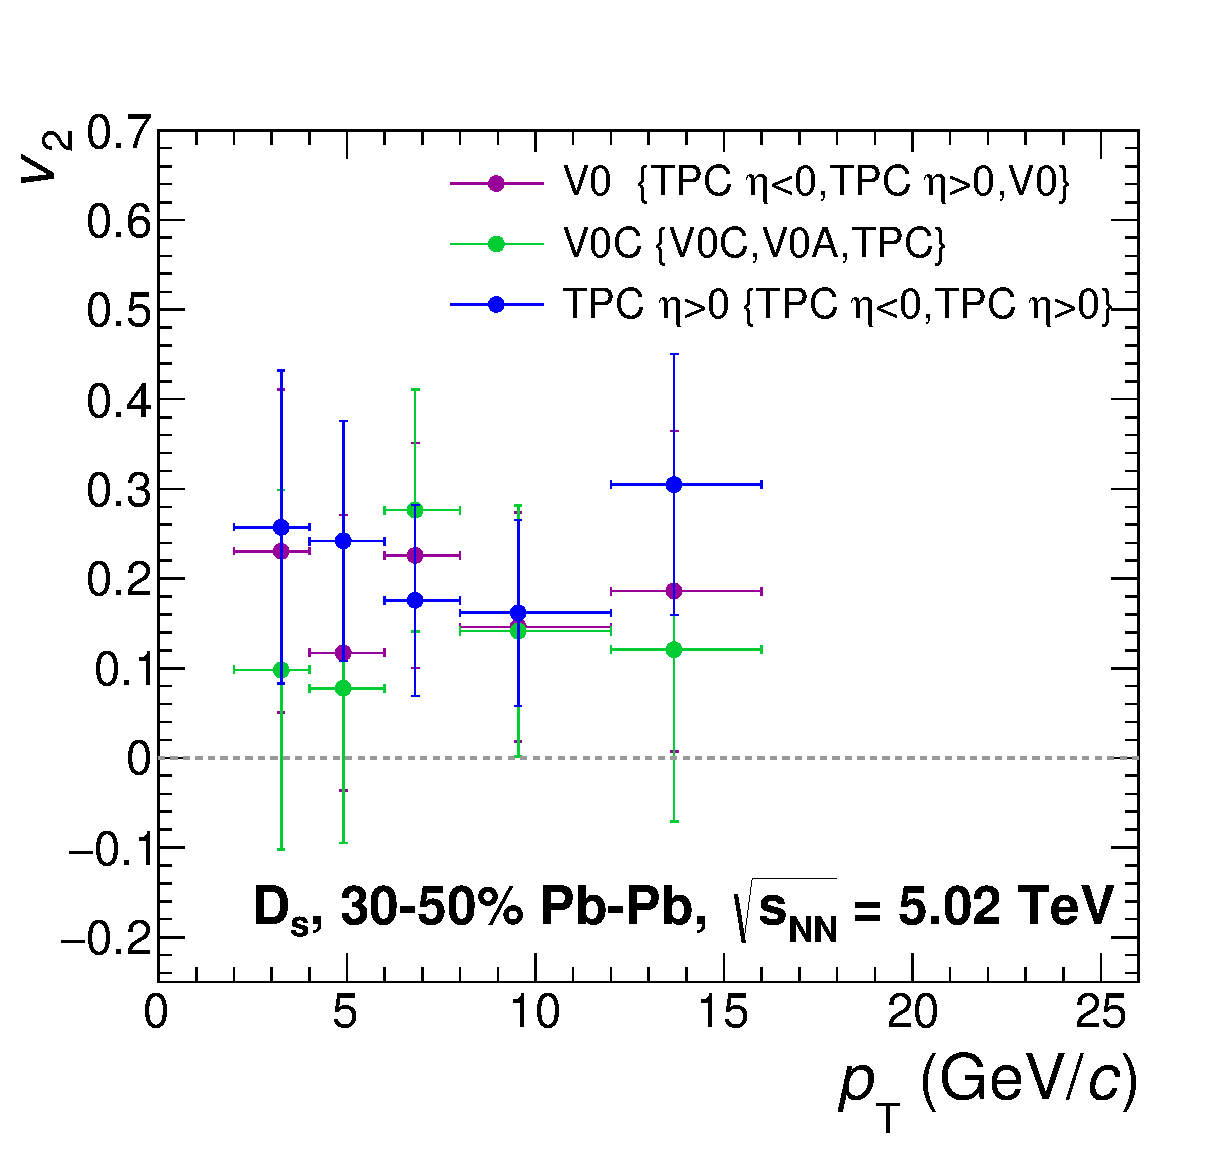
\includegraphics[width=0.45\textwidth]{FigCap5/v2_diffDetComparison.eps}
 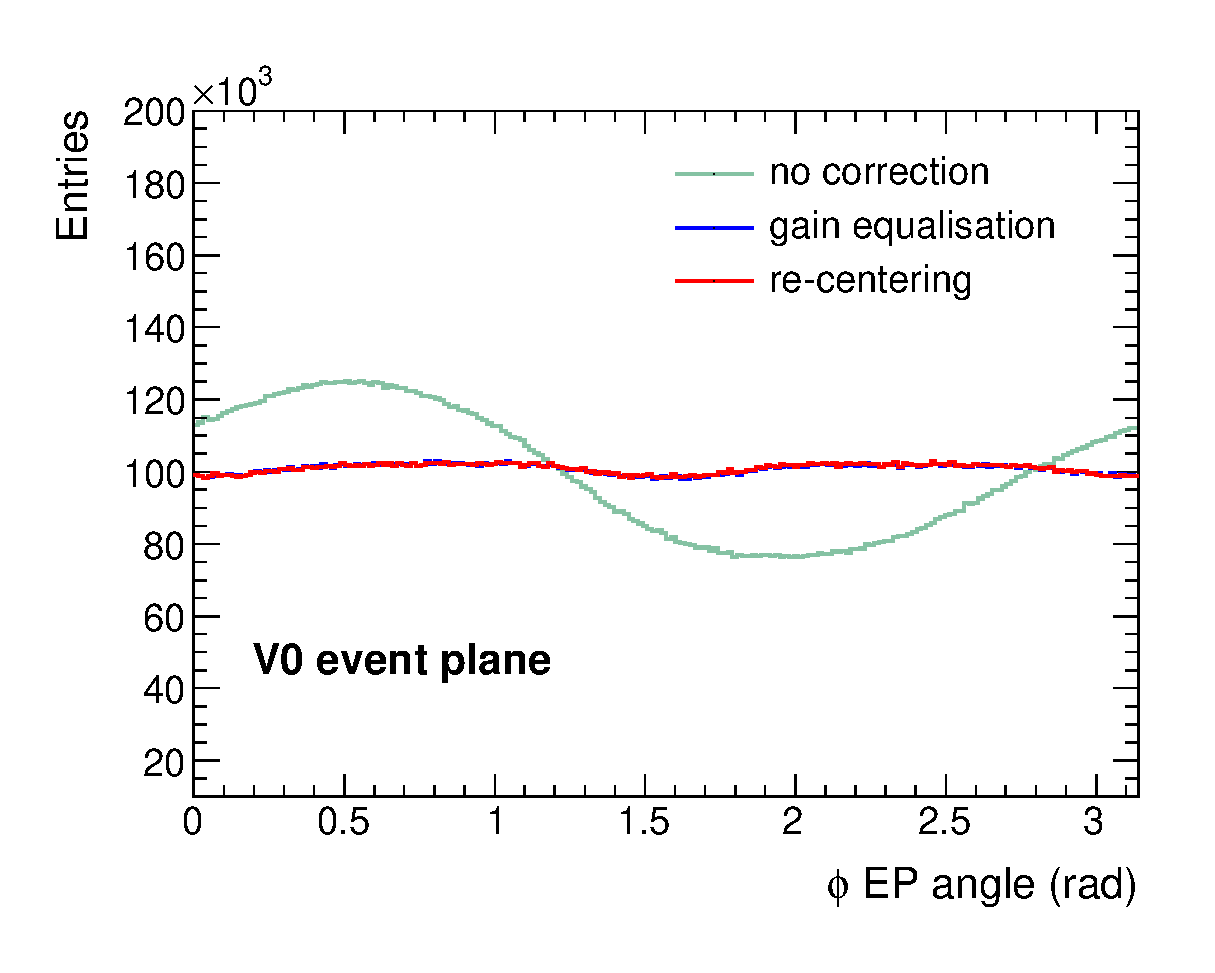
\includegraphics[width=0.53\textwidth]{FigCap5/V0EvPlaneDitrib.eps}
 \caption{Left: $\Ds$ $v_2$ calculated with different detector configurations. Right: event-plane angle distributions obtained with the V0 detector without corrections and after gain equalisation, re-centering and alignment corrections.}
   \label{fig:QoverMCalibration}
\end{figure}



The distribution of the event plane angles recorded by an ideal detector is completely
flat, since there is not a preferred direction for the $\Psi_{RP}$ angle.
Effects of non-uniformity of the detector performance and tracking efficiency (in the case of the TPC) 
can generate a non-flat distribution of the event plane angle. 
For this purpose, a gain equalisation of individual 
V0 detector channels was applied, correcting the raw amplitudes $M_c$ 
as: $M_c' = M_c / \langle M_c \rangle$, where $\langle M_c \rangle$ is the average amplitude
of the V0 channels in intervals of $z$ vertex z and V0A(C) multiplicity. 
A re-centering of the distributions of the components
of $\vec{Q}_n$ vector ($X_n$, $Y_n$) can also be applied, by subtracting
the ($\langle X_n\rangle$, $\langle Y_n \rangle$) values averaged over all events:
\begin{equation}
\begin{split}
\emph{{X}}_n' =& \emph{X}_n - \langle \emph{X}_n \rangle,\\
\emph{{Y}}_n' = &\emph{Y}_n - \langle \emph{Y}_n \rangle.
\end{split}
\end{equation}
Further corrections can be introduced but, as shown in the right panel of 
Fig.~\ref{fig:QoverMCalibration}, already the re-centering
procedure, applied after the gain equalisation, does not provide a substantial improvement.
The $\vec{Q}_n$ vector was normalised to the
multiplicity M of the event to reduce the sensitivity to multiplicity
fluctuations. 


\subsection{Event-plane based methods for $v_2$ extraction} 
\label{sec:epMethodsDescript}
The basic principle in flow analysis is to quantify the azimuthal 
anisotropies via Fourier coefficients obtained through a 
decomposition of the azimuthal distributions of reconstructed particles in a Fourier series (see Eq.~\ref{eq:fourier}).
The $v_2$ coefficient of D mesons can be obtained by integrating Eq.~\ref{eq:fourier}
in two $\Delta \varphi$ intervals and including a correction for the
resolution. In the analysis presented here, the sample of candidates was 
divided in two $\Delta\phi = \varphi_{\rm D}-\psi_n$ regions: the \textit{in-plane} 
and the \textit{out-of-plane} regions. We define the in-plane 
region (centred on the event plane) as the region 
$\left(-\frac{\pi}{4},\frac{\pi}{4}\right]\cup\left(\frac{3\pi}{4},\frac{5\pi}{4}\right]$ and
 the out-of-plane as $\left(\frac{\pi}{4},\frac{3\pi}{4}\right]\cup\left(\frac{5\pi}{4},\frac{7\pi}{4}\right]$. 
 In each $\Delta\phi$ interval the $\Ds$ yield is extracted via
an invariant-mass fit. Resolving Eq.~\ref{eq:fourier} for the number of $\Ds$ measured 
 in the in-plane and out-of-plane regions separately we obtain:
\begin{equation}\label{eq:ninout}
 \begin{split}
  & N_\text{in-plane} = k\int_\text{in-plane}1+2v_2\cos(2\Delta \varphi)d\Delta \varphi = k'\cdot(\pi+4v_2)\\
  & N_\text{out-plane} = k\int_\text{out-plane}1+2v_2\cos(2\Delta \varphi)d\Delta \varphi= k'\cdot(\pi-4v_2),
 \end{split}
\end{equation}
and therefore it is possible to compute $v_2$ from the relative 
difference between the number of $\Ds$ mesons observed in-plane and out-of-plane:
\begin{equation}
\label{eq:anis}
 v_2 = \frac{1}{R_2} \frac{\pi}{4}\frac{N_\text{in-plane}-N_\text{out-plane}}{N_\text{in-plane}+N_\text{out-plane}}.
\end{equation}
The contribution of all odd harmonics, 
as well as $v_4$ and $v_8$, to the $v_2$ value induce the same average 
contribution to $N_\text{in-plane}$ and $N_\text{out-of-plane}$ 
due to symmetry, and therefore they do not affect $v_2$ calculated with 
Eq.~\ref{eq:anis}. The contribution of $v_6$, $v_{10}$ and higher 
harmonics is assumed to be negligible based on the 
values measured for light-flavour hadrons~\cite{Aamodt:2011by,ATLAS:2012at}.
The factor $\frac{1}{R_2}$ in Eq.~\ref{eq:anis} is the correction for the finite resolution in the
estimate of the symmetry plane $\Psi_2$ via the event plane $\psi_2$.
 Simulations showed that the D-meson reconstruction 
 and selection efficiencies do not depend on $\Delta\varphi$~\cite{Abelev:2014ipa}, 
therefore Eq.~\ref{eq:anis} can be applied using the 
D-meson raw yields, without an efficiency correction.

 \subsection{In- and out-of-plane signal extraction}
 \label{sec:SigExtracV2}
 The topological selections used for the selection of $\Ds$ candidates in the 30-50\% centrality class
 are very similar to those reported in Table~\ref{tab:topologicalselections_ds_3050} for the
 $\varphi$-integrated yields in the same centrality class.
 Only the selections on NDL$_{\rm xy}$, $\sigma_{vertex}$, $\Delta M$ 
 and $|\cos^3 \theta^\prime({\rm K})|$ were slightly released in some $\pt$
 intervals. The invariant-mass distributions were analysed separately for $\Dsplus$ candidates
 in the in-plane and out-of-plane $\Delta \varphi$ intervals, 
with the event plane determined with the V0 
in the 30-50\% centrality class, as shown in Fig.~\ref{fig:deltaphibinsds} 
as an example for the interval $6 < \pt < 8 \, \Gevc$.
To extract the $\Ds$ raw yield, the invariant mass distribution was fitted using a two Gaussian
functions to model the $\Ds$ peak and the contribution of the $\DplustoKKpi$ and 
an exponential shape to model the background.
The mean and the width of the Gaussians were fixed to those obtained from a fit to
the invariant-mass distribution integrated over $\Delta \varphi$, 
where the signal has higher statistical significance. 
Fig.~\ref{fig:deltaphibinsds} shows the values of Gaussian means and 
widths for the in-/out-of-plane and the $\varphi$-integrated extracted yields.
The yields in the two $\varphi$ regions were extracted in five $\pt$ 
intervals between 2 and 16 $\Gevc$.
The values of the extracted raw yields and the signal-over-background 
ratios for the in-plane and out-of-plane invariant-mass fits 
are reported in Table~\ref{signalsDs}.

\begin{figure}
\centering
 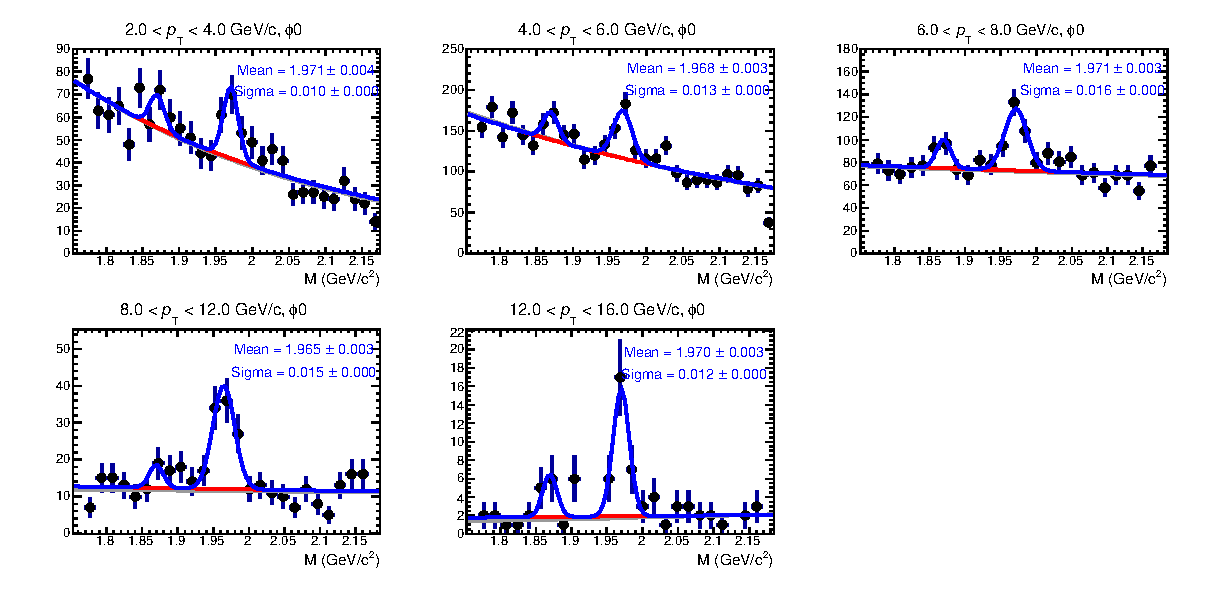
\includegraphics[width=1\textwidth]{FigCap5/InvMassDs_Phi0_3050.eps}
\caption{$\Dspm$ in-plane invariant-mass distributions in the analysed $\pt$ intervals.}
\label{fig:deltaphi0binsds}
\end{figure}
\begin{figure}
\centering
 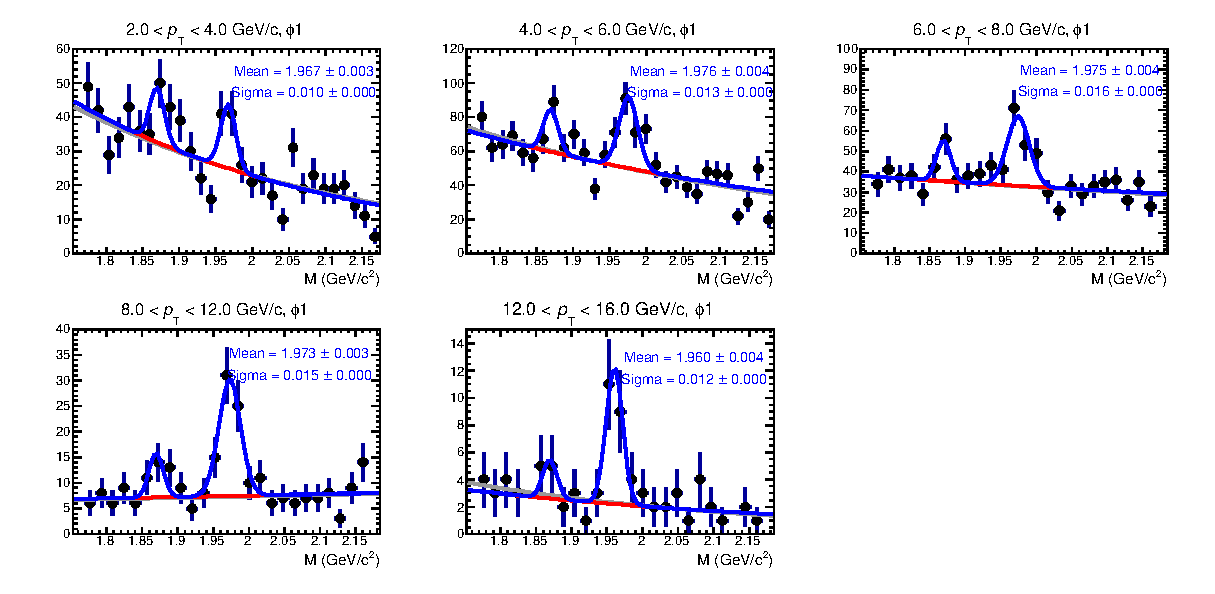
\includegraphics[width=1\textwidth]{FigCap5/InvMassDs_Phi1_3050.eps}
\caption{$\Dspm$ out-of-plane invariant-mass distributions in the analysed $\pt$ intervals.}
\label{fig:deltaphi1binsds}
\end{figure}
\begin{figure}
\centering
 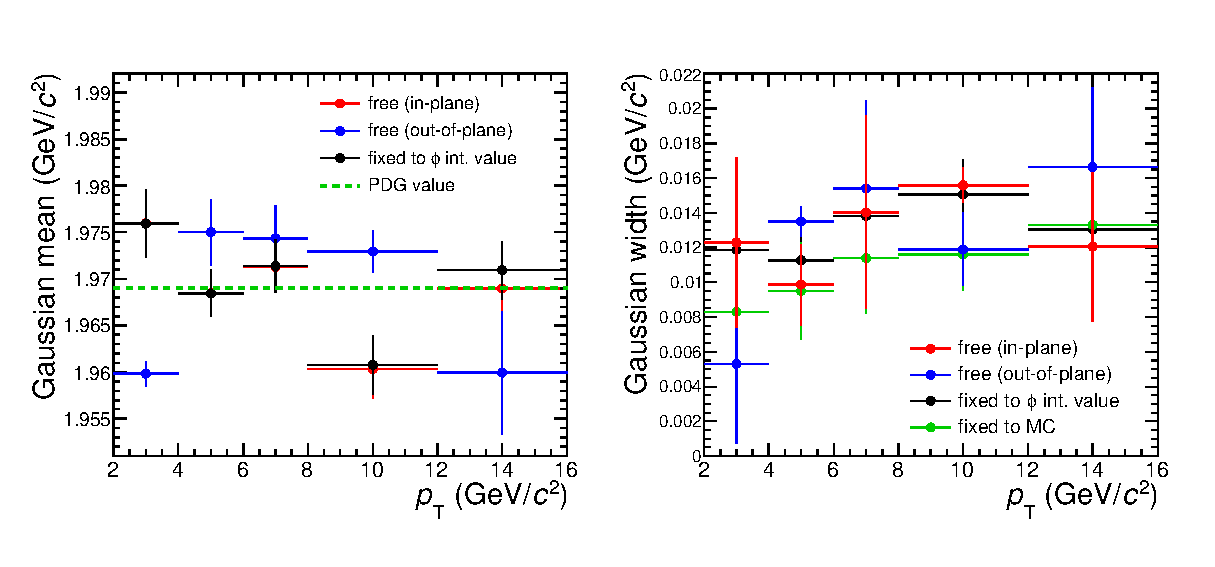
\includegraphics[width=.98\textwidth]{FigCap5/sigmaComparison.eps}
\caption{Position (left) and widths (right) of the Gaussian peak in the $\Ds$ candidate invariant-mass fits for $\varphi$-integrated, in-plane and out-of-plane samples. In the left panel, the value of $\Ds$ mass from PDG is also shown (dashed green line).}
\label{fig:deltaphibinsds}
\end{figure}

\begin{table}[!h]
 \begin{center}
  \begin{tabular}{|c|c|c|c|c|}
\hline
\multirow{2}{*} {$\pt$ ($\GeV/c$)}  & \multicolumn{2}{c|}{In-plane} & \multicolumn{2}{c|}{Out-of-plane} \\
\cline{2-5} & raw yield & S/B & raw yield & S/B\\
\hline
2-4 & $58 \pm 14$ & 0.31 & $34 \pm 11$  & 0.31 \\
\hline
4-6 & $135 \pm 24$  & 0.21 & $97 \pm 18$  & 0.35\\
\hline
6-8 & $134 \pm 21$  & 0.31  & $83 \pm 15$  & 0.43 \\
\hline
8-12 & $70 \pm 11$  & 0.99 & $57 \pm 10$  & 1.36\\
\hline
12-16 & $25 \pm 6$  & 3.00 & $18 \pm 5$  & 1.89 \\
\hline
  \end{tabular}
 \caption{$\Dspm$ raw yields and signal-over-background ratios in the different $\pt$ intervals and $\Delta\varphi$ regions.}
 \label{signalsDs}
 \end{center}
\end{table}  

\subsection{B feed-down subtraction}
\label{sec:FDv2}
The measured $\Dspm$ meson raw yield includes a contribution (of about 90\%)
from prompt $\Ds$ mesons and a contribution from beauty feed-down.
Considering that $v_2$ is an additive quantity, the measured $v_2$ is therefore given by:
\begin{equation}
\label{eq:bfeed}
v_2^{\rm obs}=f_{\rm prompt} v_2^{\rm promptD} + (1-f_{\rm prompt})v_2^{\rm feed-down}.
\end{equation}
The value of $f_{\rm prompt}$ is estimated via Eq.~\ref{eq:fprAA} using FONLL calculations for B meson
cross sections, the B$\rightarrow$D decay kinematics from the EvtGen package and
the Monte Carlo efficiencies for feed-down D mesons and a
hypothesis for the $\RAA^{\rm feed-down}$, which is the same used for
$\RAA$ analyses and discussed in Sec.~\ref{sec:CorrectionsAA}.
To calculate $v_{\rm 2}^{\rm prompt}$, a hypothesis on 
$v_{\rm 2}^{\rm feed\textnormal{-}down}$ is used.
The measured $v_2$ of non-prompt J/$\psi$~\cite{Khachatryan:2016ypw} 
and the available model calculations~\cite{Aichelin:2012ww,Uphoff:2012gb,Greco:2007sz} 
suggest that $0<v_{\rm 2}^{\rm feed\textnormal{-}down}<v_{\rm 2}^{\rm prompt}$.
The lower limit, $v_2^{\rm feed-down}=0$, corresponds to the extreme assumption case in which:
\begin{itemize}
\item{at low $\pt$, where $v_2$ is determined by collective flow, 
$b$ quarks do not take part in the collective expansion and hence do 
not contribute to the observed D-meson anisotropy;}
\item{at high $\pt$, where $v_2$ is determined by 
energy loss, due to different path lengths for quarks emitted in-plane and out-of-plane,
$b$ quarks are not affected by the medium.}
\end{itemize}
The upper limit, $v_2^{\rm feed-down}=v_2^{\rm prompt}$, implies that:
\begin{itemize}
\item{at low $\pt$, $b$ quarks are flowing as $c$ quarks;}
\item{at high $\pt$, $b$ and $c$ quarks lose same amount of energy interacting with 
the medium (i.e. no effect due to the different quark mass).}
\end{itemize}
Assuming a uniform probability distribution of $v_{\rm 2}^{\rm feed\textnormal{-}down}$ in this interval,
the central value for $v_{\rm 2}^{\rm prompt}$ is calculated 
considering:
\begin{equation}
\label{eq:hypoFD}
v_{\rm 2}^{\rm feed\textnormal{-}down}=v_{\rm 2}^{\rm prompt}/2,
\end{equation}
thus:
\begin{equation}
\label{eq:finalv2}
v_{\rm 2}^{\rm prompt}= 2\,v_{\rm 2}^{\rm obs}/(1+f_{\rm prompt}).
\end{equation}

\section{Systematic uncertainties on $v_2$}
\label{sec:systsectionV2}
The main sources of systematic uncertainty affecting the measurement of 
$v_2$ are related to: 
\begin{itemize}
\item signal extraction from the invariant-mass
distributions;
\item centrality dependence of the resolution term $R_2$;
\item non-flow effects;
\item B feed-down subtraction;
%\item residual non-flatness of the event plane.
\end{itemize}

\subsection{Yield extraction systematics}
\label{sec:rawYv2}
The systematic uncertainty on the yield extraction was 
estimated by testing different fit configurations.
Fits were performed by varying: (i) background fit functions
(exponential, first and second order polynomial functions), 
(ii) lower and upper limits in the fit, (iii) Gaussian peak widths free or fixed to the value
extracted from the $\varphi$-integrated distribution. Furthermore, the yield was defined by
counting the histogram entries in the invariant-mass region of the signal, after subtracting the background
contribution estimated from a fit to the side bands. The distributions of
residuals between the $i^{th}$ trial and the reference $v_2$ value, 
$v_2^{trial}-v_2^{ref}$, were obtained in each $\pt$ interval and are shown in Fig.~\ref{fig:residualsV2}. 
The systematic uncertainty was assigned
considering both the shift with respect to zero and the RMS of the residual
distributions. The absolute values of this uncertainty range from 
0.015 to 0.070 for $\Ds$ mesons, depending on the $\pt$ interval.
\begin{figure}
\centering
  \includegraphics[width=1\textwidth]{FigCap5/plotResidualPhiYieldExtr.eps}
\caption{Residual distributions of $v_2$ values from multiple-trial procedure for in-plane and out-of-plane yield extraction and default $v_2$ values. The three distributions refer to yield extraction via fit with Gaussian width left as free parameter (red), fixed to the values from the $\varphi$-integrated distribution (black) and to extraction via bin counting method (green).}
\label{fig:residualsV2}
\end{figure}

\subsection{Event Plane resolution}
\label{sec:EPreso}
The event-plane resolution correction factor $R_2$ depends on the 
collision centrality~\cite{Abelev:2014ipa}. The left-hand panel of Fig.~\ref{fig:EtaGapSyst} shows
the resolution $R_2$ of the event plane determined from the V0 detector as a function of the centrality in the interval
30-50\%. The resolution was computed using three sub-events, i.e. the
V0 and the TPC tracks in two different $\eta$ intervals,
with and without the introduction of a 
pseudo-rapidity gap between the two considered TPC regions.
The resolution decreases from $\approx 0.83$ to $\approx 0.70$ with increasing centrality
percentile.
The value of resolution used in Eq.~\ref{eq:anis} was computed
 assuming a uniform distribution of the D-meson yield within 
 the 30-50\% centrality class.
 To estimate the systematic uncertainty, this value was 
 compared with those obtained from two alternative approaches
based on weighted averages of the $R_2$ values in narrow centrality 
intervals, using as weights either the measured $\Dzero$-meson yields or the number of 
nucleon-nucleon collisions from the Glauber model. 
A systematic uncertainty of 2\% on $R_2$ was estimated from 
this study.
\begin{figure}
\centering
  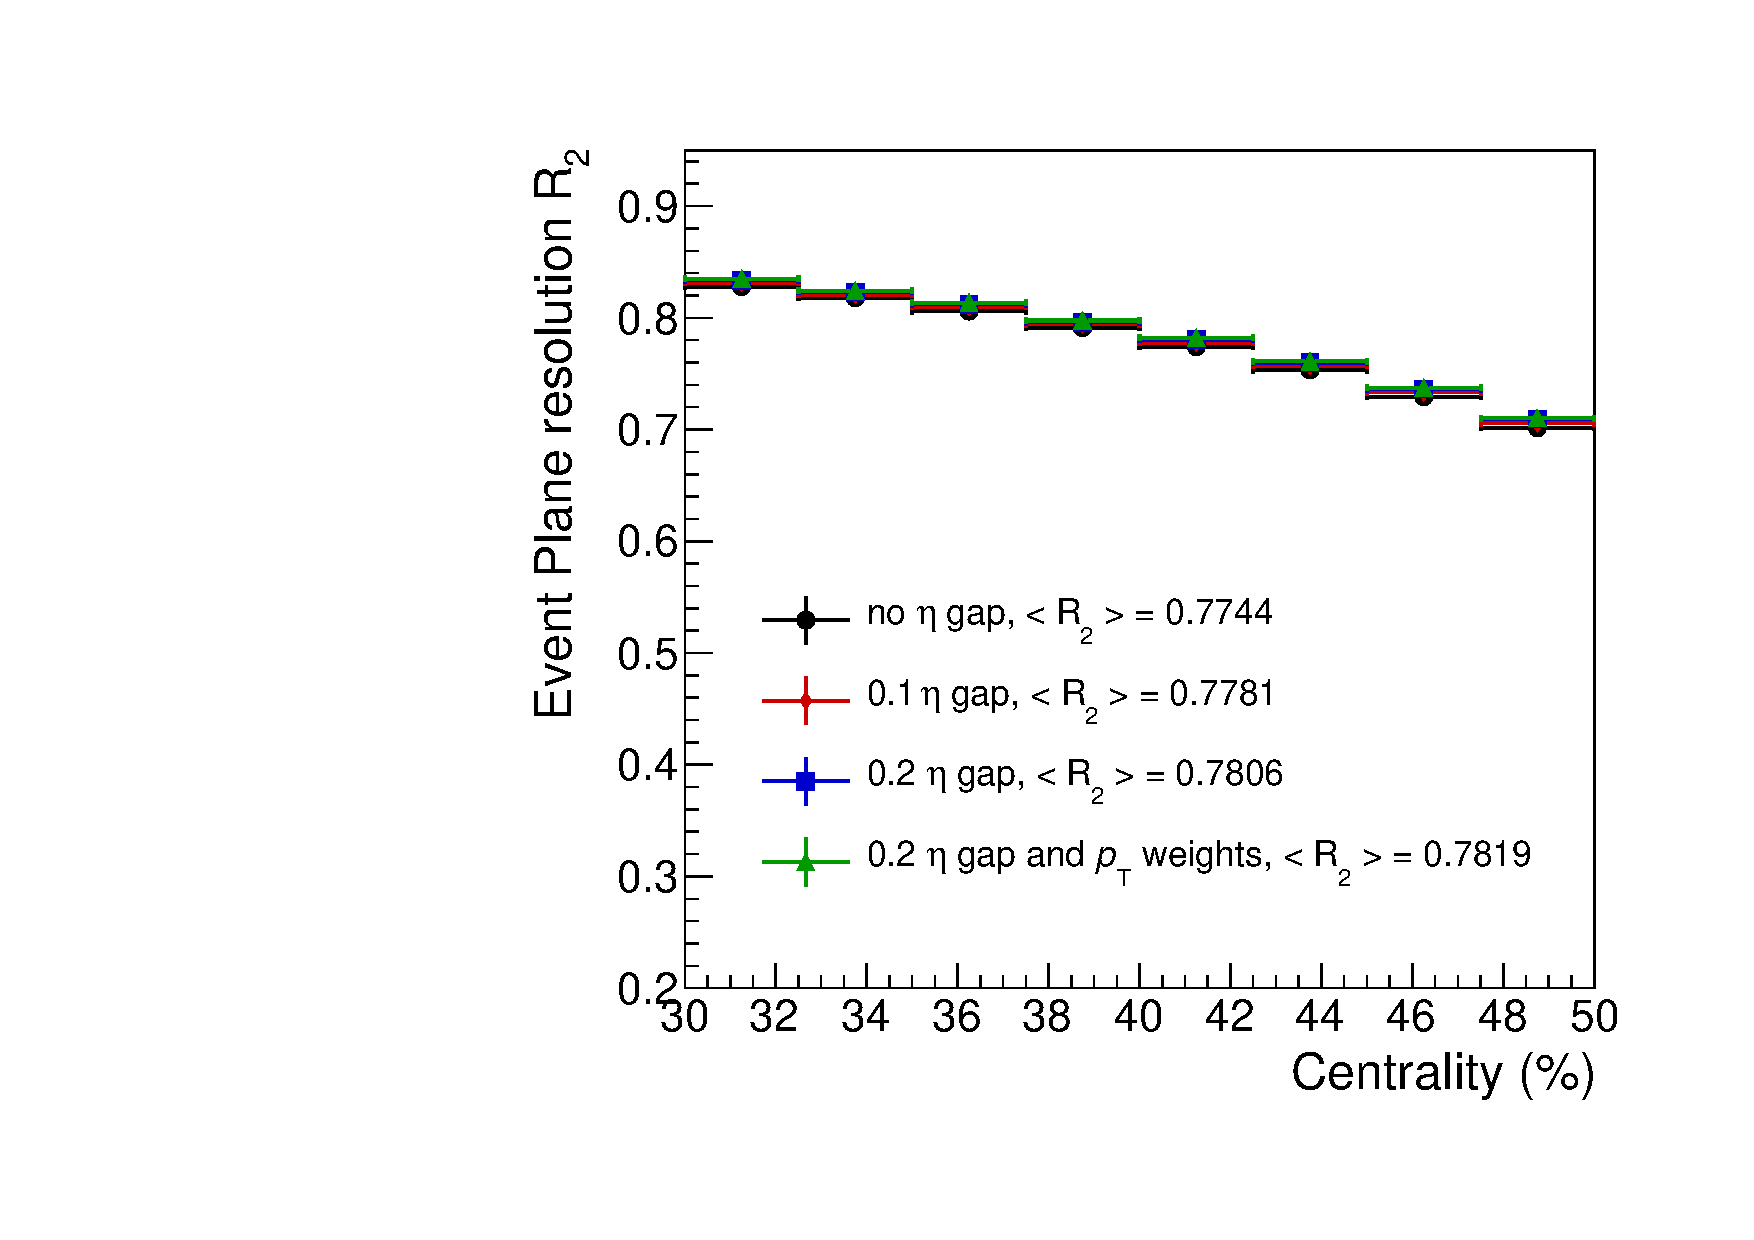
\includegraphics[width=.49\textwidth]{FigCap5/EPresolution_VZERO_NonFlowSyst.pdf}
  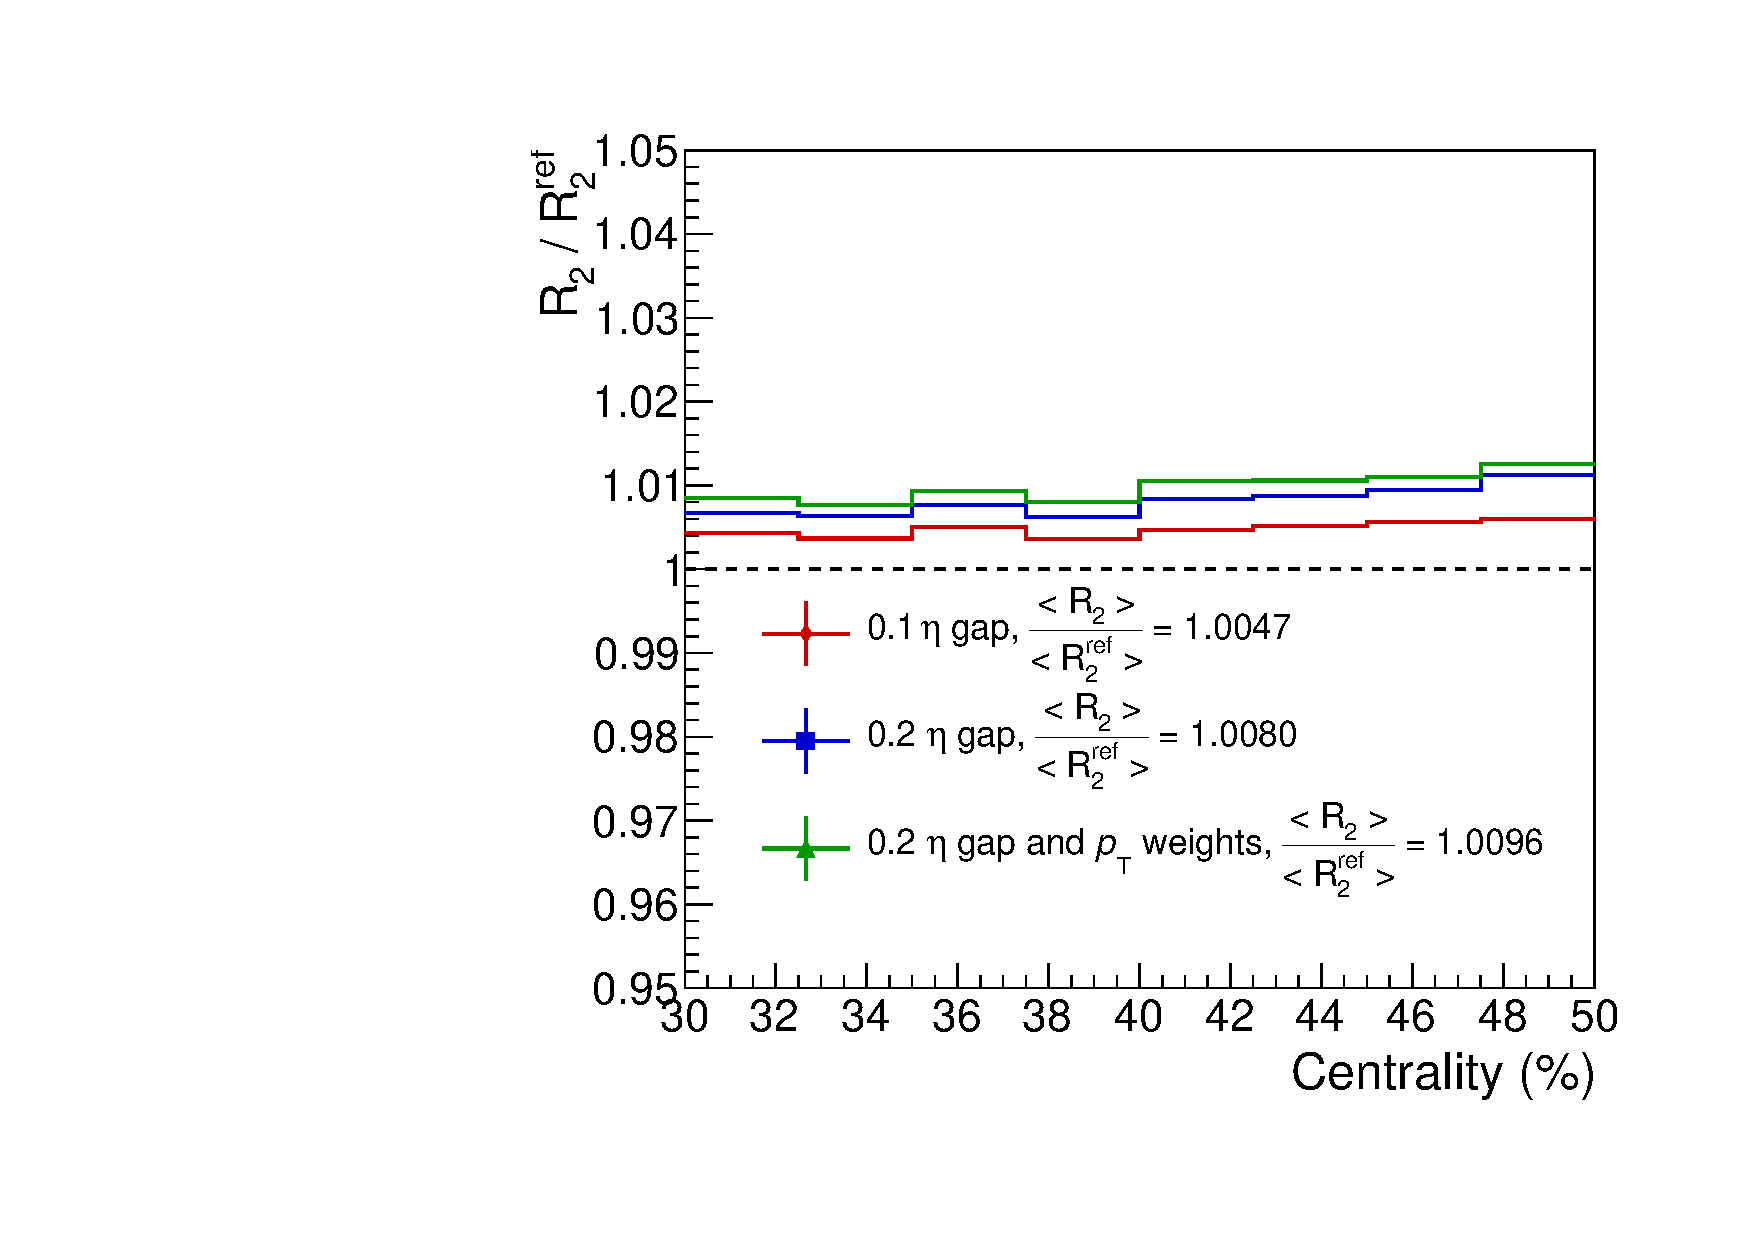
\includegraphics[width=.49\textwidth]{FigCap5/EPresolution_VZERO_NonFlowSyst_ratio.pdf}
\caption{Event plane resolution as a function of centrality (left) estimated introducing an eta gap between the sub-events computed using the TPC tracks and the corresponding relative variation with respect to the default configuration (right).}
\label{fig:EtaGapSyst}
\end{figure}

\subsection{Non-flow contributions}
\label{sec:NonFlow}
In order to estimate a possible bias in the $R_2$ correction factor due to non-flow correlations among the three 
event planes used for the resolution estimates,
the resolution was re-computed introducing 
a pseudo-rapidity gap between the TPC sub-events. 
In particular it was considered an eta 
gap of 0.1 and 0.2 units between the samples of the TPC tracks with positive/negative 
eta. The left panel of Fig.~\ref{fig:EtaGapSyst} shows
 the comparison of the event plane resolution
as a function of centrality computed without eta gap, 
with an eta gap of 0.1 units, with an eta gap 0.2 units. 
In the latter case the resolution was also computed 
applying per-track $\pt$ weights in the calculation of the $\vec{Q}_2$ vector with
the tracks reconstructed in the TPC.
In the right panel of Fig.~\ref{fig:EtaGapSyst} the corresponding 
relative variation of the event plane resolution is shown and the effect integrated over the 
30-50\% centrality class is reported in the legend. Considering this observation, an additional 1\%
 systematic uncertainty on the determination of the
event plane resolution was assigned.
\iffalse
\subsection{EP flatness}
\label{sec:EPflat}
In order to check the flatness of the event plane 
distributions several checks have been performed 
for the main configuration used (main event plane 
measured with the multiplicity in the full V0 and
 resolution estimated with 3 sub-events). In particular, if we consider that
\begin{equation}
\cos(2\Delta\phi) = \cos(2\phi_D-2\psi_{EP}) = \cos(2\phi_D)\cos(2\psi_{EP})+\sin(2\phi_D)\sin(2\psi_{EP}),
\end{equation}
where $\phi_D$ is the azimuthal angle of the D meson 
and $\psi_{EP}$ the azimuthal angle of the event plane, 
a non-zero value of 
$< \cos(2\phi_D) >/R_2 \times < \cos(2\psi_{EP}) >/R_2$ 
(and the same for the sine) would lead to a bias in the 
measurement of the D-meson $\vtwo$. The  
$< \cos(2\psi_{EP}) >$ and $< \sin(2\psi_{EP}) >$ factors 
have been extracted from the fits to the event plane 
distributions shown in Fig.. The fitting functions used are respectively 
\begin{equation}
N(1+2b\cdot \cos(2\psi_{EP}))
\end{equation}
and 
\begin{equation}
N(1+2b'\cdot \sin(2\psi_{EP})),
\end{equation}
where $b = < \cos(2\psi_{EP}) >$ and $b' = < \sin(2\psi_{EP}) >$.
In particular for the full V0, we can observe how the parameters 
extracted with this method are smaller than 0.001.


To estimate $< \cos(2\phi_D) >$ and $< \sin(2\phi_D) >$ 
have been used two methods:
\begin{itemize}
\item The subtraction of the $\cos(2\phi_D)$ ($\sin(2\phi_D)$) 
distribution of the combinatorial background from the distributions of the side-bands.
\item The fit of the $\cos(2\phi_D)$ ($\sin(2\phi_D)$) vs. the invariant-mass.
\end{itemize}
\fi
\begin{figure}
 \centering
 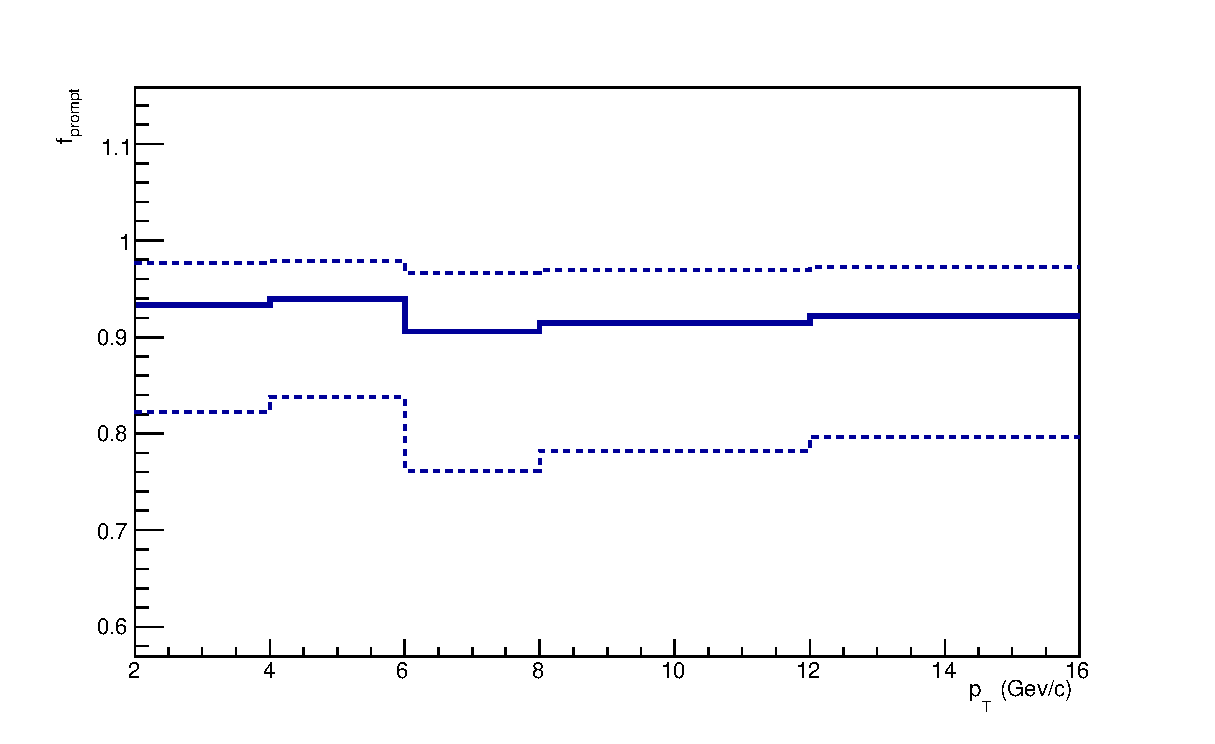
\includegraphics[width=9cm]{FigCap5/fprompt_3050.eps}
\caption{Values of prompt fraction for $\Ds$ mesons in the 30-50\% centrality class.}
\label{fig:fPrompt}
\end{figure}

\subsection{Feed down systematics}
\label{FDsystV2}
The systematic uncertainty on $v_{2}^{\rm prompt}$ due to the subtraction of the feed-down contribution 
is estimated by varying the central value of 
$v_{2}^{\rm feed\textnormal{-}down}=v_{2}^{\rm prompt}/2$ by $ \pm v_{2}^{\rm prompt}/\sqrt{12}$, corresponding to 
$\rm \pm 1\,RMS$ of a uniform distribution in $(0,\,v_{2}^{\rm prompt})$.
The value of $v_2^{\rm prompt}$ is computed as:
\begin{equation}
v_{2}^{\rm prompt}=v_{2}^{\rm obs}/f_{\rm prompt} - (1-f_{\rm prompt})/f_{\rm prompt}v_{2}^{\rm feed-down}.
\end{equation} 
The maximum and minimum values of $v_2^{\rm prompt}$ were
obtained using respectively the minimum and the maximum values 
of $v_{\rm 2}^{\rm feed-down}$ and $f_{\rm prompt}$. 
The uncertainty on $f_{\rm prompt}$ is obtained from the
variation of the renormalisation and factorisation scales and of the charm quark
mass in the FONLL calculation, and from the variation of the 
$R_{\rm AA}^{\rm feed\textnormal{-}down}$ hypothesis in  
$\frac{1}{3}< R_{\rm AA}^{\rm feed\textnormal{-}down}/R_{\rm AA}^{\rm prompt}<3$~\cite{Adam:2015jda}. 
The values of $f_{\rm prompt}$ of $\Ds$ mesons
are shown in Fig.~\ref{fig:fPrompt} and the error bars include the
contributions of the FONLL scales variations and of the variation of
the $\RAA$ hypothesis. The value of the absolute systematic uncertainty on $v_2$
due to the correction of the feed-down contribution, which includes also the variation
of the hypothesis on $v_{\rm 2}^{\rm feed-down}$, ranges from 0.001 to 0.030 depending on the $\pt$ interval.
\begin{figure}[!t]
 \begin{center}
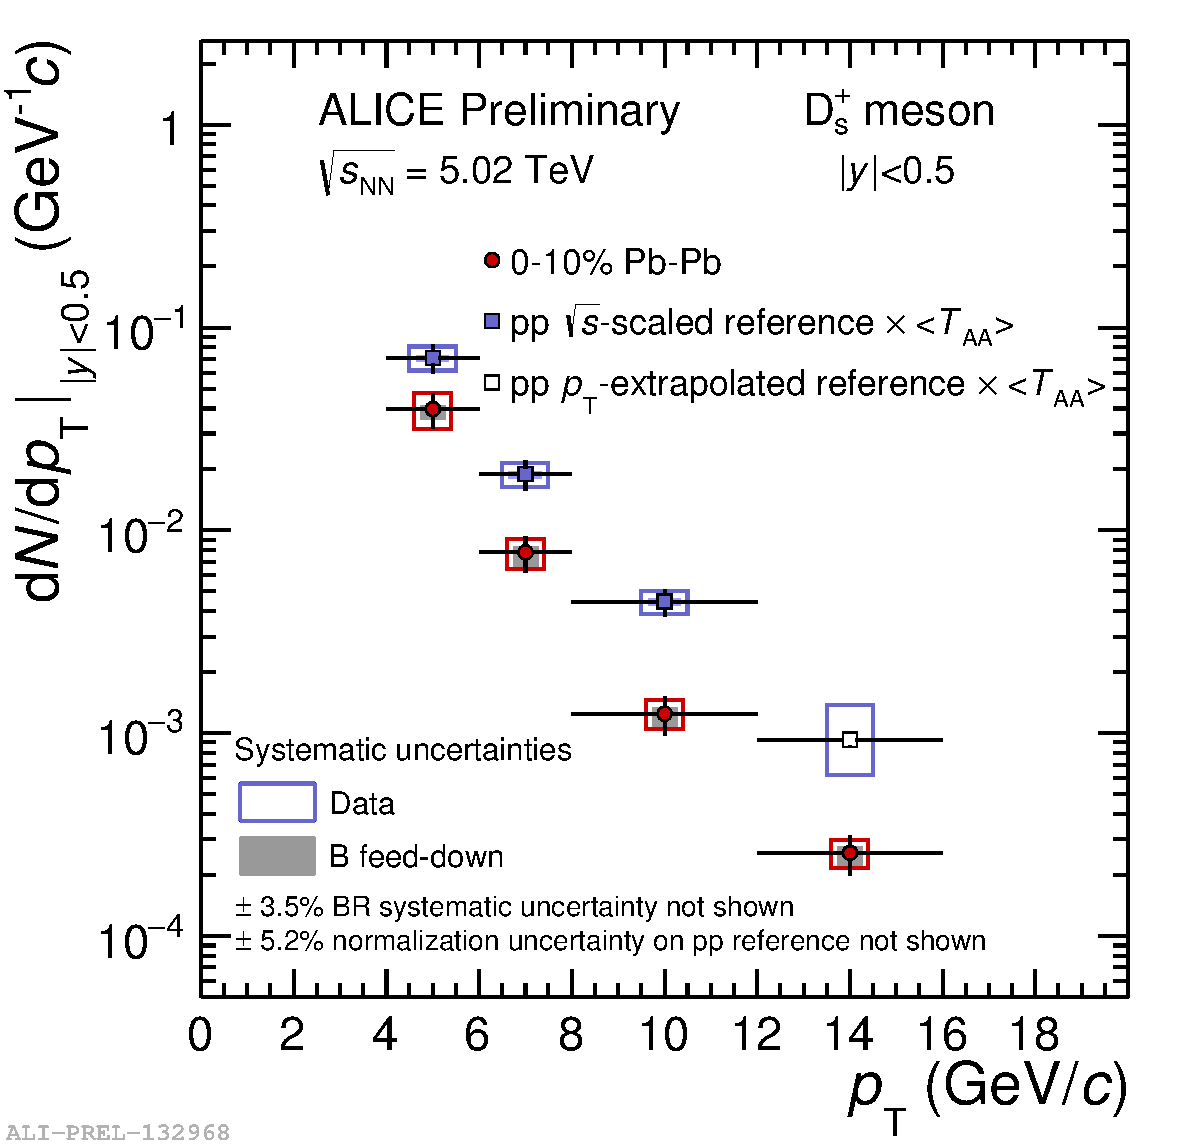
\includegraphics[width=.49\textwidth]{FigCap5/Ds_dNdpt_010.pdf}
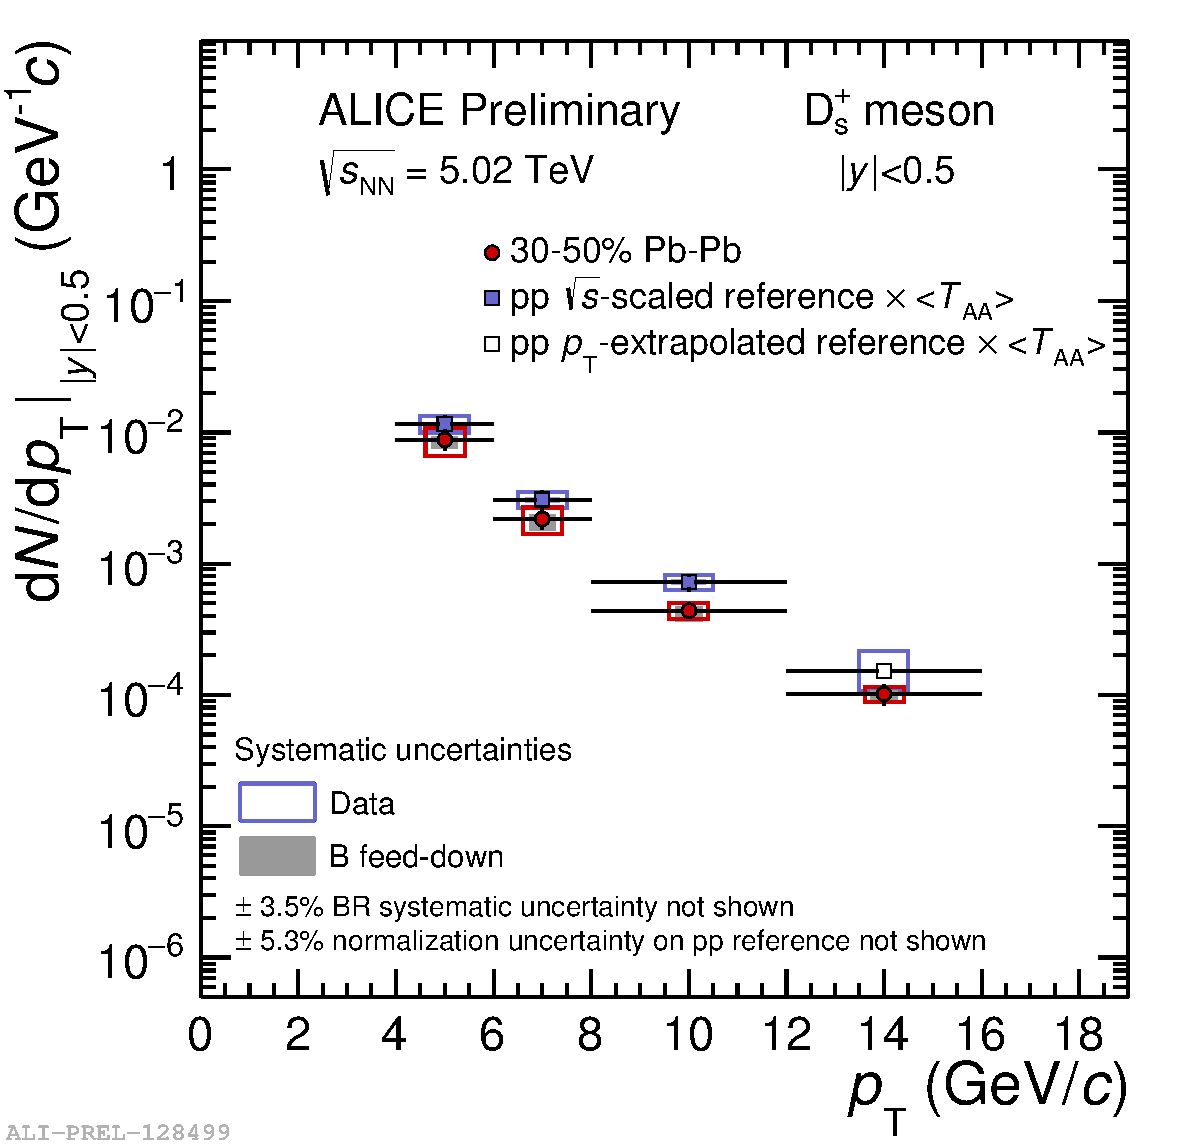
\includegraphics[width=.49\textwidth]{FigCap5/Ds_dNdpt_3050.pdf}
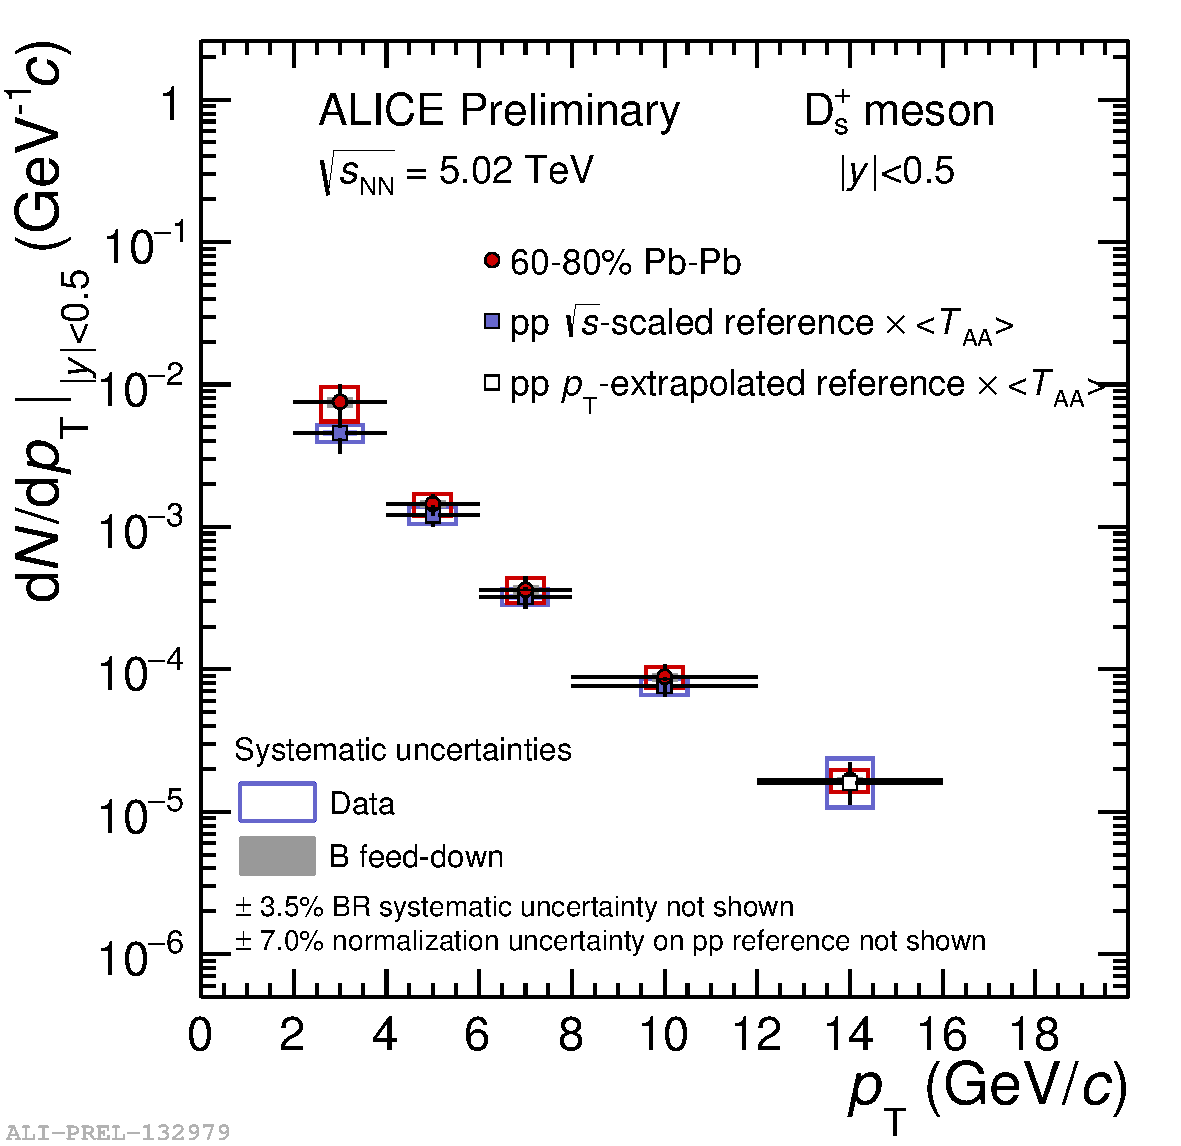
\includegraphics[width=.49\textwidth]{FigCap5/Ds_dNdpt_6080.pdf}
 \end{center}
 \caption{Transverse momentum distributions d$N$/d$\pt$ of 
prompt $\Ds$ meson in the 0--10\%, 30--50\% and 60--80\% 
centrality classes in $\PbPb$ collisions 
at $\sqrtsNN=5.02~\tev$. }
 \label{fig:DmesCorrYields010} 
\end{figure} 

\section{Results}
\label{sec:PbPbResults}
The transverse-momentum distributions d$N$/d$\pt$ of prompt $\Dsplus$ mesons in Pb-Pb
collisions at $\sNN=5.02$ TeV are shown in Fig.~\ref{fig:DmesCorrYields010}
for the 0-10\%, 30-50\% and 60-80\% centrality classes. 
They are compared to the corresponding cross-section in pp collisions at the same centre-of-mass energy
multiplied by the $\langle T_{\rm AA} \rangle$ of the considered centrality class.
The vertical bars represent the statistical uncertainties, the empty boxes
the systematic uncertainties from the data analysis, and the shaded boxes
the systematic uncertainty due to the subtraction of the feed-down from 
B-hadron decays. The uncertainty on the branching ratios is quoted separately.
The points of the d$N$/d$\pt$ in Pb-Pb collisions have empty markers in the interval $12 < \pt < 16 \, \Gevc$,
because they are obtained with the $\pt$-rescaled reference.
The $\Ds$ yields in Pb-Pb collisions show a suppression relative to the pp reference
yields in the 0-10\% and 30-50\%. The suppression increases with increasing centrality percentile
and with the transverse momentum.\\
%Uncertainties on the pp cross section
%normalisation and on the branching ratios are quoted separately.


The production yields of the different D-meson species were studied by computing
the ratios of the d$N$/d$\pt$ of $\Dzero$, $\Dplus$ and $\Ds$ mesons in Pb-Pb collisions
and comparing them to those measured in pp collisions at $\s = 7 $ TeV.
The results for the $\Ds/\Dzero$ and $\Ds/\Dplus$ ratios are shown in the top panels of
Fig.~\ref{fig:DmesRatio}. For comparison, the ratios of 
non-strange D-meson yields ($\Dplus$/$\Dzero$, $\Dstar$/$\Dzero$) are shown in the bottom panels.
The $\Dplus$/$\Dzero$ and $\Dstar$/$\Dzero$ ratios are compatible in Pb-Pb and pp collisions, 
indicating no significant modification of their relative abundances. 
In the ratios involving the charmed strange $\Ds$ meson a hint of difference is observed.
The central values of the $\Ds/\Dzero$ and $\Ds/\Dplus$ ratios are larger in Pb-Pb than in pp collisions, 
in all three centrality classes, however no strong conclusion can be drawn because the measurements in the two systems 
are compatible within about one standard deviation of the combined statistical and systematic uncertainties.
It is also worth noting that the measurements in Pb-Pb collisions at $\sNN = 5.02$ TeV reported
here are more precise than the ones at $\sNN = 2.76$ TeV of Ref.~\cite{Adam:2015jda}, thanks to the larger
data sample in the semi-peripheral classes and the improvements in the analysis.\\

\begin{figure}[!h]
 \begin{center}
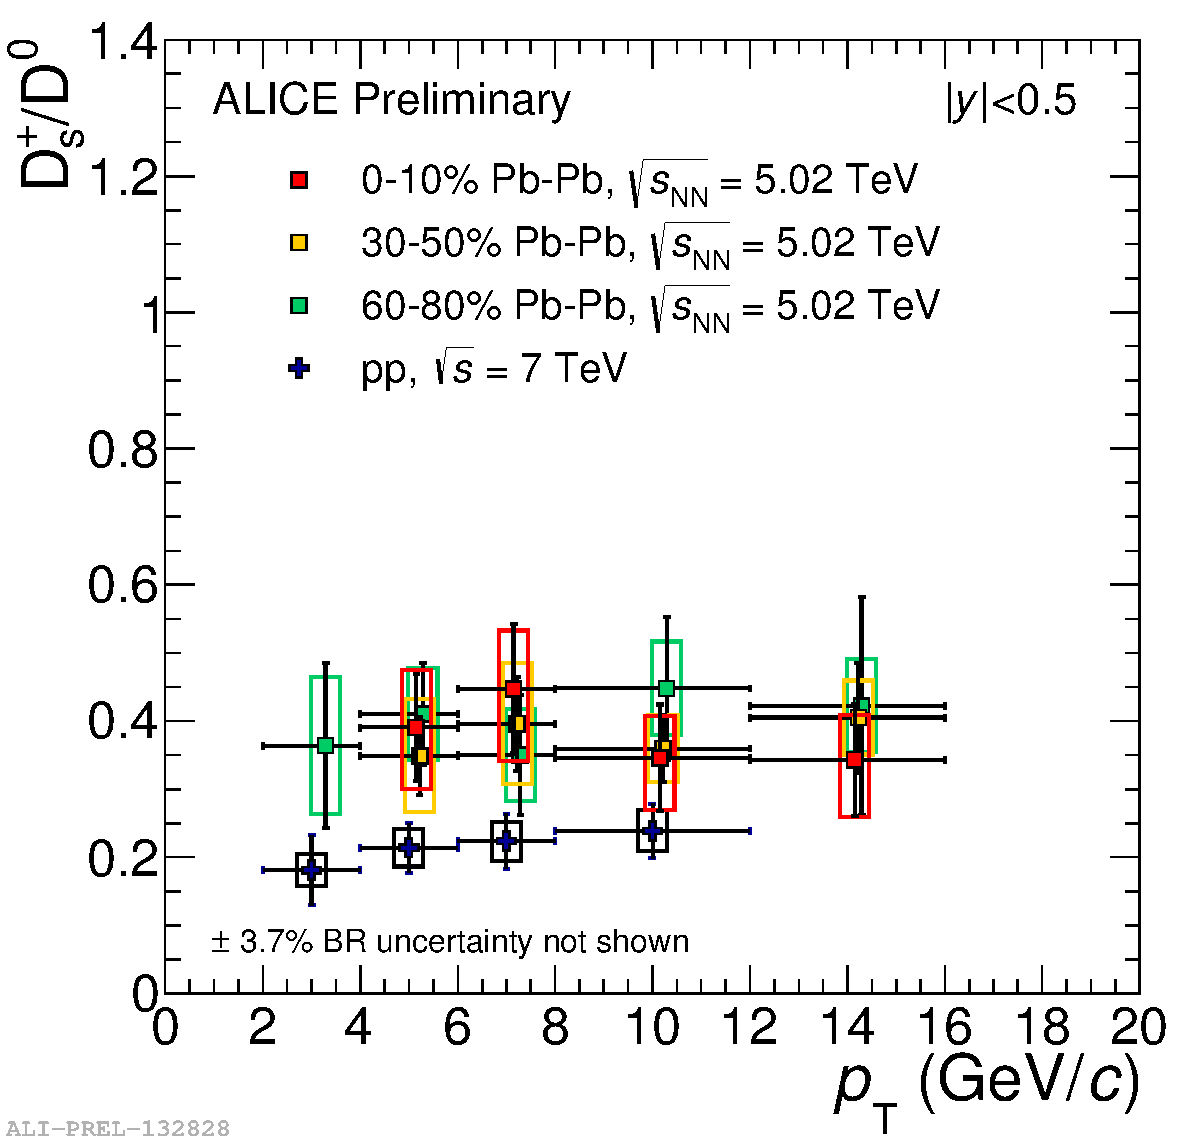
\includegraphics[width=0.49\textwidth]{FigCap5/RatioDsD0-PbPb-010-3050-6080-502-pp-7.pdf}
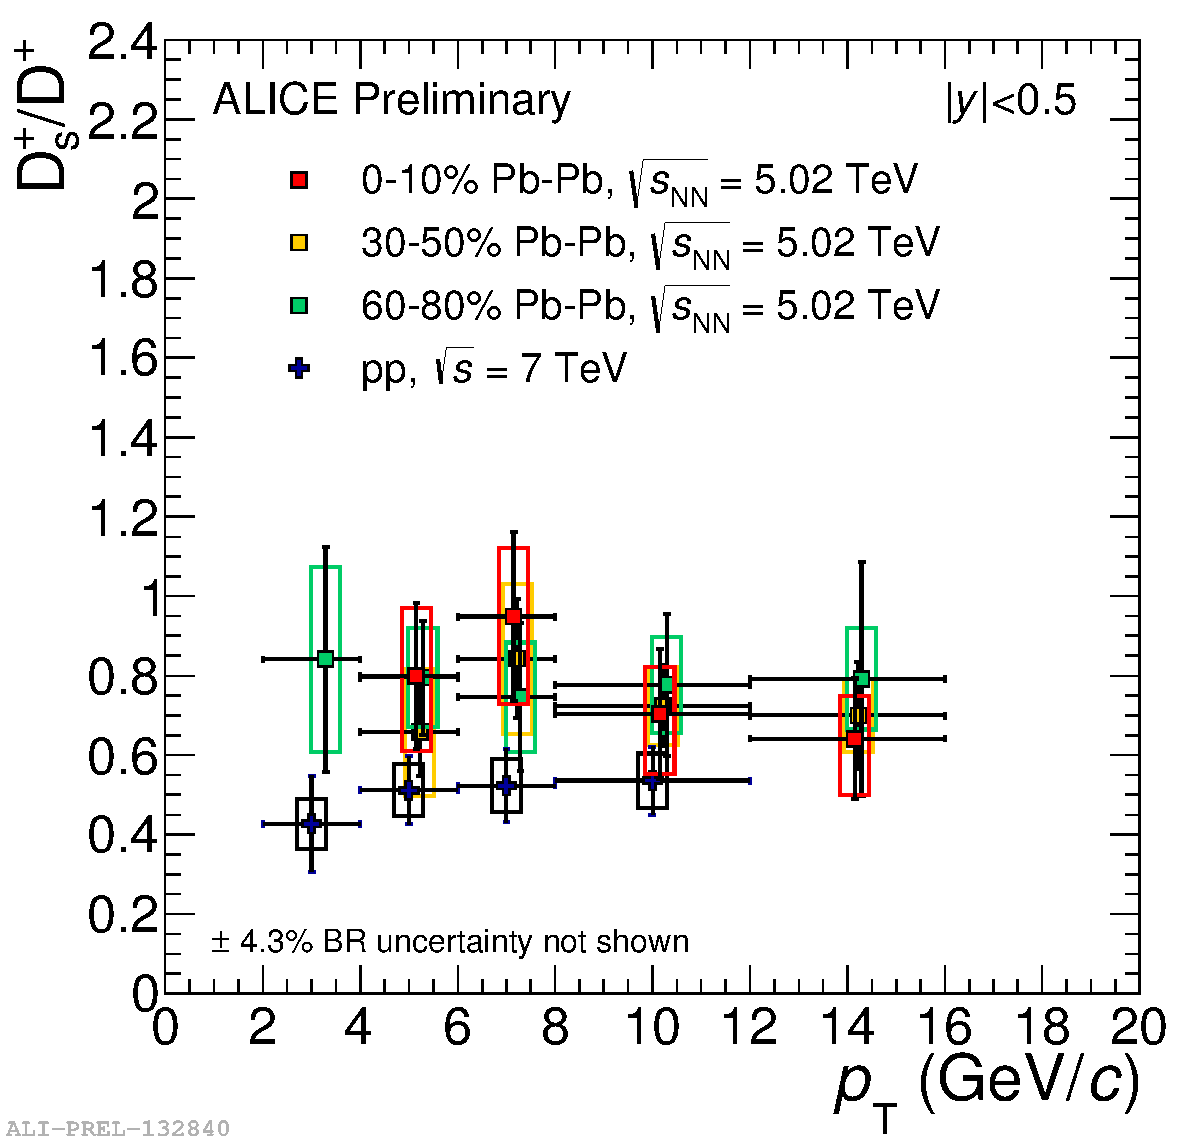
\includegraphics[width=0.49\textwidth]{FigCap5/RatioDsDplus-PbPb-010-3050-6080-502-pp-7.pdf}
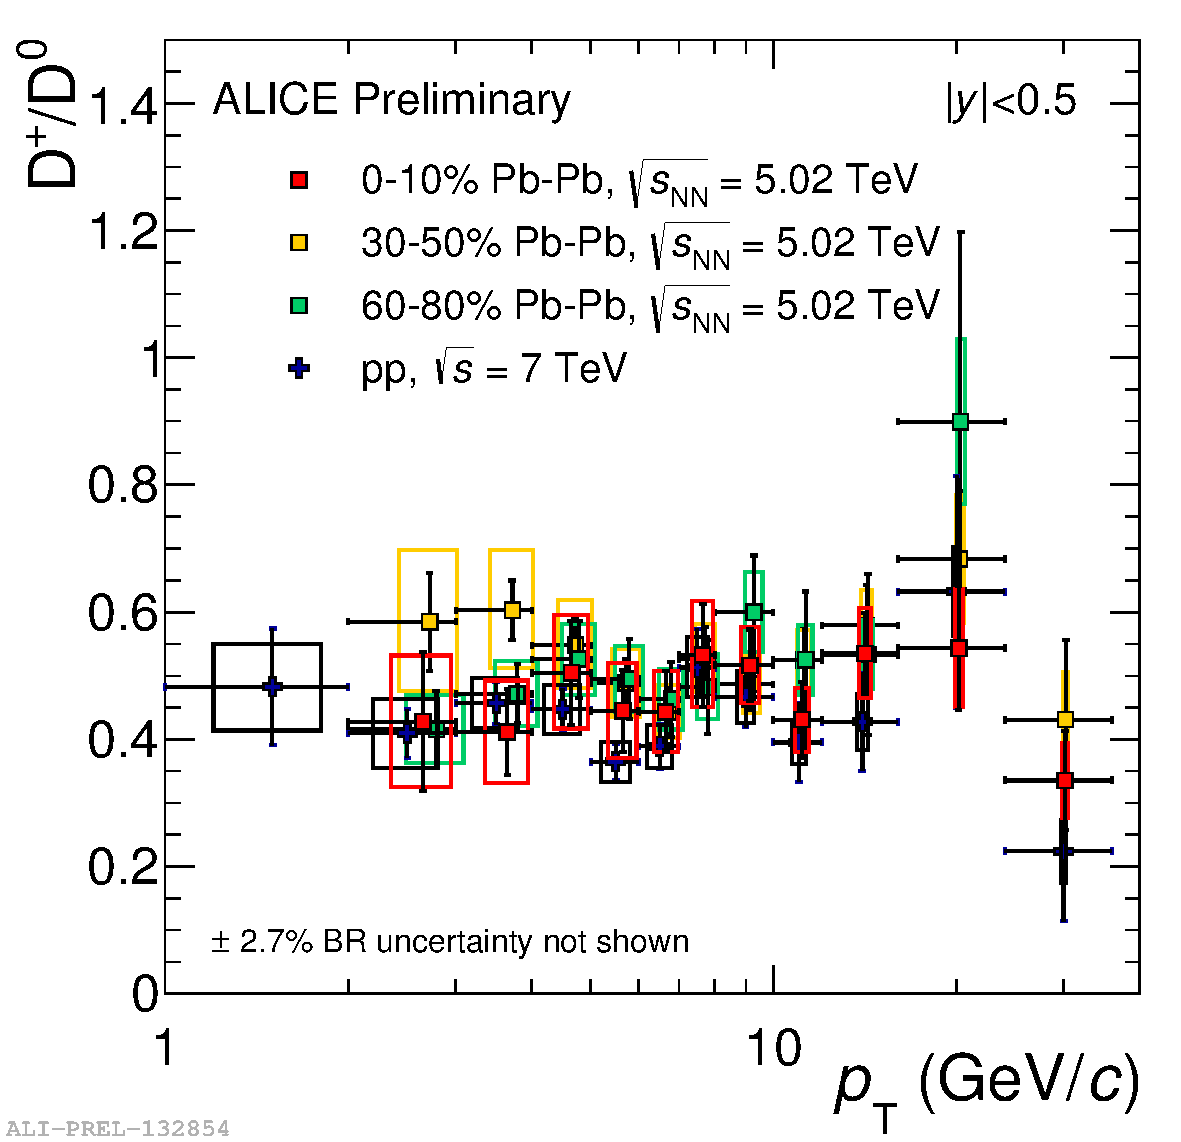
\includegraphics[width=0.49\textwidth]{FigCap5/RatioDplusDzero-PbPb-010-3050-6080-502-pp-7.pdf}
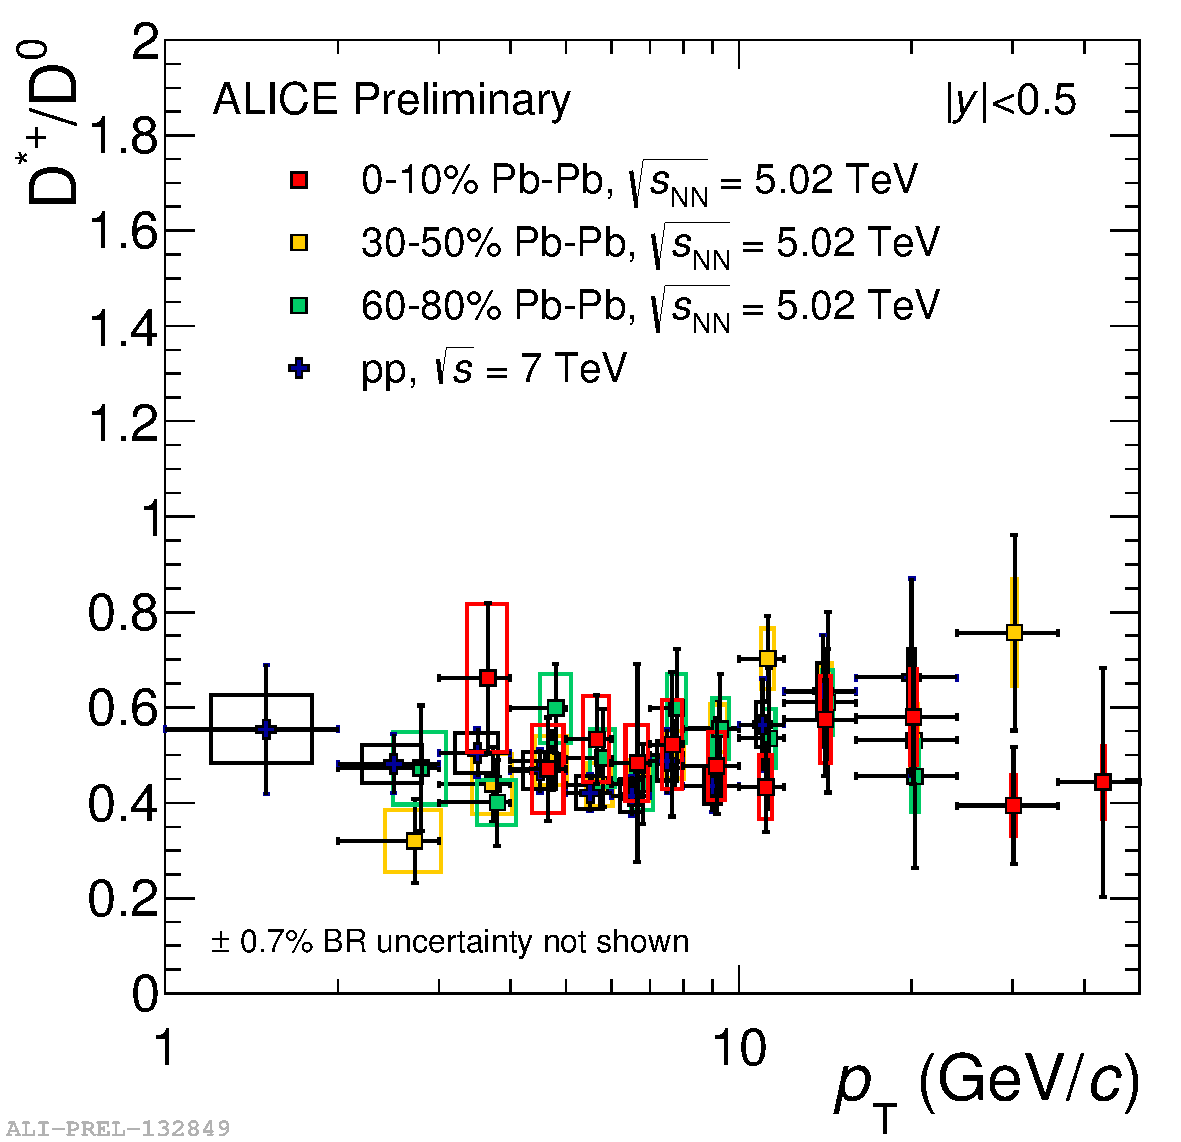
\includegraphics[width=0.49\textwidth]{FigCap5/RatioDstarDzero-PbPb-010-3050-6080-502-pp-7.pdf}
 \end{center}
 \caption{Ratio of prompt D-meson yields as a function of $\pt$.
Statistical (bars) and systematic (boxes) uncertainties are shown.}
 \label{fig:DmesRatio} 
\end{figure} 

\begin{figure}[!h]
\centering
\includegraphics[angle=0, width=0.45\textwidth]{FigCap5/DmesonAverageDs_010.pdf}
\includegraphics[angle=0, width=0.45\textwidth]{FigCap5/DmesonAverageDs_3050.pdf}
\includegraphics[angle=0, width=0.45\textwidth]{FigCap5/DmesonAverageDs_6080.pdf}
 \caption{$\RAA$ 
  of prompt $\Dsplus$ mesons 
  compared with the average $\RAA$ of $\Dzero$, $\Dplus$ and $\Dstar$ mesons for the 
0--10\%, 30--50\% and 60--80\%. 
Statistical (bars),  systematic (empty boxes), and normalisation (shaded box) 
uncertainties are shown.}
 \label{fig:DmesRaa} 
\end{figure} 


The magnitude of the suppression observed in the d$N$/d$\pt$ in Pb-Pb relative to pp collisions 
can be estimated by looking at the nuclear modification factor presented in Fig.~\ref{fig:DmesRaa}.
The $\Raa$ of prompt $\Dsplus$ mesons is shown, for the three different centrality classes,
in Fig.~\ref{fig:DmesRaa}, where it is compared to the average $\Raa$ of non-strange 
D mesons. The $\Dsplus$ nuclear modification factors in the 0--10\% 
and 30--50\% centrality classes show a suppression that is
maximal at $\pt=6$--$10~\gev/c$, where a reduction of the yields by
a factor of about 3 and 1.5 with respect to the binary-scaled
 pp reference is observed in the two centrality classes, respectively.
The average $\RAA$ in the 60--80\% centrality class is compatible 
with unity, without a pronounced dependence on $\pt$.
 The central values of the $\RAA$ of $\Ds$ mesons are larger than those of non-strange D mesons but the 
differences between the strange and non-strange D-meson $\RAA$ are 
of about one standard deviation of the combined statistical and systematic
uncertainties, as in the case of the ratios shown in Fig.~\ref{fig:DmesRatio}.
Therefore, no strong conclusion can be drawn on the predicted difference of $\Ds$ and 
non-strange D-meson nuclear modification factor in presence of hadronisation
via charm quark recombination in the QGP.\\




In Fig.~\ref{fig:DandDsRaaWithModels},  the non-strange and 
strange D-meson $\RAA$ are compared with  
the PHSD~\cite{Song:2015ykw} and 
 TAMU~\cite{He:2014cla} models that provide a calculation for both observables. A larger
 $\RAA$ of $\Ds$ mesons as compared to non-strange D mesons is expected in the two models, in particular for $\pt<5~\gev/c$.
Both the calculations are based on heavy-flavour transport with the Langevin approach.
In TAMU the interactions of the charm quarks with the medium include only collisional (i.e.\,elastic) processes, 
while in PHSD~\cite{Song:2015ykw} also energy loss from medium-induced gluon radiation
is considered, in addition to collisional processes.
In the models, the enhancement of $\Ds$ $\RAA$ with respect to that of non-strange D mesons at low $\pt$ is induced 
by charm-quark recombination with strange quarks in the QGP.
It is interesting to note that the TAMU model (see Fig.~\ref{fig:DandDsRaaWithModels}) predicts a larger effect than the 
 PHSD model and this is due to the fact that in TAMU the enhancement
of strange-quark production in heavy-ion relative to pp collisions is considered.
The central values of the measured $\RAA$ of strange and non-strange D mesons differ also 
at $\pt \approx 10~\gev/c$, although the present experimental 
uncertainties prevent us from drawing a firm conclusion. This 
difference is absent in the PHSD model. In the TAMU model the difference  
becomes smaller at $\pt > 10 \, \Gevc$, because the fragmentation mechanism (universal in pp and Pb-Pb) dominates in this region and 
leads to similar $\RAA$ for D and $\Ds$ mesons. The small residual splitting is induced by an extra suppression of D mesons
due to interactions in the hadronic phase, which are expected to be small for $\Ds$ mesons~\cite{He:2012df} and
neglected in the calculations. 
\\


\begin{figure}[!t]
 \begin{center}
\includegraphics[angle=0, width=0.49\textwidth]{FigCap5/DmesonAverageDs_010_Models.pdf}
 \end{center}
 \caption{Average $\RAA$ of $\Dzero$, $\Dplus$ and $\Dstar$ mesons and $\RAA$ of $\Ds$ mesons in the 0--10\% centrality class compared with the PHSD~\cite{Song:2015ykw}  and TAMU~\cite{He:2014cla} model calculations.}
 \label{fig:DandDsRaaWithModels} 
\end{figure} 




The $v_2$ of prompt $\Ds$ mesons in
the 30--50\% centrality class is shown as a function of $\pt$ in Fig.~\ref{fig:v2_Ds}.
The symbols are positioned at the average $\pt$ of the 
reconstructed $\Ds$ mesons in the considered $\pt$ interval. This $\langle \pt \rangle$ value was determined as the 
average of the $\pt$ distribution of candidates in the signal invariant-mass region, 
after subtracting the contribution of the background 
candidates estimated from the side bands.
The average $v_2$ of $\Ds$ meson in
 the intervals $2<\pt<8~\gev/c$ is $\langle v_2 \rangle = (0.226 ^{+0.138}_{-0.088})$,
where the uncertainty was calculated using quadratic error propagation for the
 statistical and uncorrelated systematic uncertainties 
(signal extraction) and linear propagation for the correlated 
systematic uncertainties ($R_2$ and feed-down correction). The average $v_2$ results
 positive with a significance of 2.6\,$\sigma$ of its uncertainty.
The $v_2$ of $\Ds$ mesons is compared to the average $v_2$ of
$\Dzero$, $\Dplus$ and $\Dstar$ as a function of $\pt$ in the right
panel of Fig.~\ref{fig:v2_Ds}. he $v_2$ of $\Ds$ and non-strange D mesons are found
to be compatible within uncertainties.\\


In Fig.~\ref{fig:v2_models}, the measured $v_2$  is compared to theoretical calculations.
Both TAMU and PHSD predict similar $v_2$ for strange and non-strange
D mesons. In the TAMU model, the small difference between $v_2$ of $\Ds$ and that of
non-strange D mesons is due to the fact that the $\Ds$ spectra freeze out after
hadronisation, while D mesons couple to the hadronic medium,
and further enhances its $v_2$ by 30\%. Therefore,
the $v_2$ splitting between non-strange D and $\Ds$ mesons is also a promising measure of the transport
properties of the hadronic phase, although the current uncertainties do not allow to draw strong conclusions.
The TAMU model describes the magnitude of the elliptic flow, 
but fails in reproducing the shape, probably due to the missing radiative term for the energy loss. 
Larger statistical samples are essential to reduce the current
uncertainties and will allow firmer constraints on the models
via simultaneous comparison of $\RAA$ and elliptic flow $v_2$
measurements.

\begin{figure}[!t]
\begin{center}
\includegraphics[width=.49\textwidth]{FigCap5/Dsv2_3050.pdf}
\includegraphics[width=.49\textwidth]{FigCap5/D0DplusAverageDsv2_05May2017.pdf}
\caption{Elliptic flow $v_2$ as a function of $\pt$ for prompt $\Ds$ mesons 
and their charge conjugates for $\PbPb$ collisions at $\sNN = 5.02$ TeV in the centrality class 30-50\%.
Right: comparison with average non-strange D meson $v_2$ as a function 
of $\pt$, for the 30-50\% centrality class in Pb-Pb collisions. }
\label{fig:v2_Ds} 
\end{center}
\end{figure}

\begin{figure*}[!t]
\begin{center}
\includegraphics[width=.55\textwidth]{FigCap5/D0DplusAverageDsv2_modelComparison_05May2017.pdf}
\caption{$v_2$ of $\Ds$ mesons for Pb-Pb collisions at $\sNN = 5.02$ TeV in the 30-50\% centrality class compared with the PHSD~\cite{Song:2015ykw}  and TAMU~\cite{He:2014cla} model calculations.}
\label{fig:v2_models} 
\end{center}
\end{figure*}

\section{Discussion and perspectives}
\label{sec:discussionAA}
In summary, the measurements of $\Dsplus$ d$N$/d$\pt$ and $\RAA$ in the
0-10\%, 30-50\% and 60-80\% centrality classes and of $v_2$ in the 30-50\% class
in Pb-Pb collisions at $\sNN = 5.02$ TeV were presented. 
The measurement of $\Dsplus$ production can provide knowledge on 
charm-quark hadronisation inside the medium. 
A significant fraction of charm quarks could undergo hadronisation 
via in-medium coalescence at intermediate and low momentum~\cite{Greco:2003vf}. 
Furthermore, an enhancement of strangeness production with respect to 
pp collisions was long suggested as a possible signal of QGP formation~\cite{Rafelski:1982pu}. 
Strange and multi-strange hadron enhancement was observed from SPS to 
LHC energy, showing a dependence on the strangeness content of the 
particles and also on the collision centrality~\cite{ALICE:2017jyt,Appelshauser:1998va,Abelev:2007xp,Abelev:2013haa}.
 The possibility of coalescence 
of charm quarks with the medium constituents, together with the possible strangeness 
enhancement, should lead to a larger relative abundance of $\Ds$ mesons compared 
to non-strange D mesons when going from pp to Pb-Pb collisions~\cite{He:2012df}.\\



The measured ratios of $\Dsplus$ to non-strange D meson yields show higher central values in Pb-Pb collisions,
for all the centrality classes, with respect to pp collisions, although the measurements are compatible
within 1$\sigma$ of the combined statistical and systematic uncertainty.
The magnitude of the suppression observed in the $\Dsplus$ d$N$/d$\pt$ in Pb-Pb  
relative to pp collisions was estimated by looking at the nuclear modification factor.
The central values of the $\Dsplus$ $\RAA$ are larger than those of 
non-strange D mesons but compatible within uncertainties. The $\Dsplus$ $\RAA$ is minimum
at $\pt=6$--$10~\gev/c$ in the 0-10\% centrality class, 
where the yields are suppressed by a factor of about 3 with respect to the binary-scaled pp reference.
The measured suppression of $\Ds$ mesons
can be described by models that include interaction of charm quarks with the medium constituents
via collisional (and radiative) processes and in-medium coalescence of charm quarks
with thermalised light quarks of the bulk. However, the current uncertainties do not allow
to discriminate among different models. To conclude about the 
predicted enhancement of the $\Dsplus$ yield relative to non-strange D mesons in 
heavy-ion collisions and about the centrality dependence of $\Dsplus$ $\RAA$, the 
uncertainties need to be reduced.
The elliptic flow of $\Dsplus$ meson was measured for the first time at LHC. The
 average $v_2$ of $\Dsplus$ is positive within 2.6$\sigma$ of the combined statistical and systematic 
 uncertainty in the interval $2 < \pt <8 \, \Gevc$. This indicates that low-momentum charm quarks take part in the
collective motion of the QGP and that collisional interaction processes as well as recombination of charm
and light quarks both contribute to the observed elliptic flow. The comparison of the $v_2$ of $\Dsplus$ and
 non-strange D mesons is also a promising test of transport properties during the hadronic phase,
 although possible effects are not appreciable with the current statistical sample.\\
 
 
 The measurements will benefit by the larger statistics of the Pb-Pb run at 
 $\sNN=5.02$ TeV that will be collected in 2018. A sample of $\sim 100$M of events in central
 collisions is expected to be recorded. This will allow to reduce the statistical uncertainty
 on the $\Dsplus$ yield in Pb-Pb from $\sim 20\%$ (current) to $\sim 6\%$ in the 
 $\pt$ interval $4 < \pt < 6 \, \Gevc$ with a rough estimate. Furthermore, with the recent pp run at the same centre-of-mass energy
 of Pb-Pb sample, the $\s$-scaling of the pp cross section will not be anymore necessary. 
 The contribution to the systematic uncertainty from the $\s$-scaling is currently $\sim4\%$ in $4 < \pt < 6 \, \Gevc$.
 Furthermore, a completely new Inner Tracking System will also be constructed for LHC Run3.
 The new detector will consists of seven layers of Monolithic Active Pixel Sensors and it will improve
 the impact parameter resolution $\sigma_{d0}$ over the full $\pt$ range, providing $\sigma_{d0}<50\,\mu$m at
 $\pt = 0.4 \, \Gevc$. The resolution of the new ITS will provides an increase of the S/B larger than 2 at low $\pt$.
The improved resolution on primary and secondary vertex reconstruction together with
the larger integrated luminosity that will be collected during the Run 3 will allow to draw firm conclusions 
about in-medium charm quark hadronisation and energy loss.
  



